\documentclass[14pt,a4paper]{extarticle}
\usepackage[utf8]{inputenc}
\usepackage{amssymb}
\usepackage[polish]{babel}
\usepackage[T1]{fontenc}
\usepackage[left=2cm,right=2cm,top=2.5cm,bottom=3cm]{geometry}

\usepackage[dvipsnames,table]{xcolor}
\usepackage{polynom}
\usepackage{tabularx}
\usepackage{amsmath}
\usepackage{amsfonts}
\usepackage{graphicx}
\usepackage{layout}
\usepackage{multirow}
\usepackage{multicol}
\usepackage{vcell}
%%%%%%%%%%%%%%%%%%%%%%%%%%%%%%%%%%%%%%%%%%%%%%%%%%%%%%%%%%%%%%%%%%%%%
%      INSBOX --- macros for inserting pictures into paragraphs     %
%       Micha\l{} Gulczy\'nski, Szczecin, Jan 1996 / Feb 1998       %
%                     mgulcz@we.tuniv.szczecin.pl                   %
%%%%%%%%%%%%%%%%%%%%%%%%%%%%%%%%%%%%%%%%%%%%%%%%%%%%%%%%%%%%%%%%%%%%%
%
%  version 2.2
%
%  available macros:
%    * \InsertBoxC{anybox}
%        insert a centered box (use int _inside_ a paragraph)
%    * \InsertBoxL{after_line}{anybox}[correction]
%    * \InsertBoxR{after_line}{anybox}[correction]
%        insert a box in the left/right after specified number of lines;
%        correction specified in square brackets is optional;
%        both macros should be called _before_ a paragraph
%    * \MoveBelowBox
%        start a new paragraph just below the current frame
%
%  see the demo.tex file for more information
%

\catcode`\@ = 11
%
%  Margin between the text and the box:
\newdimen\@InsertBoxMargin
\@InsertBoxMargin = 2mm
%
%  definition of \ParShape, an inproved version of plain \parshape
%
\newcount\@numlines    % sum: m_1+...+m_n
\newcount\@linesleft   % counter used when reading lines of \ParShape
\def\ParShape{%
    \@numlines = 0
    \def\@parshapedata{ }% here we'll collect data for plain \parshape
    \afterassignment\@beginParShape
    \@linesleft
}%
\def\@beginParShape{%
    \ifnum \@linesleft = 0
      \let\@whatnext = \@endParShape
    \else
      \let\@whatnext = \@readnextline
    \fi
    \@whatnext
}%
\def\@endParShape{%
    \global\parshape = \@numlines \@parshapedata
}%
\def\@readnextline#1 #2 #3 {% #1 #2 #3 are: m_i, leftskip_i, rightskip_i
    \ifnum #1 > 0
      \bgroup  % I want to keep changes of \dimen0 and \count0 local
        \dimen0 = \hsize
        \advance \dimen0 by -#2  % \parshape requires left skip and
        \advance \dimen0 by -#3  % _length_of_line_ (not right skip!)
        \count0 = 0
        \loop
          \global\edef\@parshapedata{%
            \@parshapedata    % add to \@parshapedata:
            #2                % left skip
            \space            % a space
            \the\dimen0       % length of line
            \space            % another space
          }%
          \advance \count0 by 1
          \ifnum \count0 < #1
        \repeat
      \egroup
      \advance \@numlines by #1
    \fi
    \advance \@linesleft by -1
    \@beginParShape
}%
%
%  \InsertBoxC, \InsertBoxL, \InsertBoxR
%
\newbox\@boxcontent     % box containing the picture to be inserted
\newcount\@numnormal    % number of leading lines to typeset normally
\newdimen\@framewidth   % width of the frame
\newdimen\@wherebottom  % position of frame's bottom
\newif\if@byframe       % true if we are just beside the frame
\@byframefalse
%
%
\def\InsertBoxC#1{%
  \leavevmode
  \vadjust{
    \vskip \@InsertBoxMargin
    \hbox to \hsize{\hss#1\hss}
    \vskip \@InsertBoxMargin
  }%
}%
\def\InsertBoxL#1#2{%
  \@numnormal = #1
  \setbox\@boxcontent = \hbox{#2}%
  \let\@side = 0
  \futurelet \@optionalparameter \@InsertBox
}
\def\InsertBoxR#1#2{%
  \@numnormal = #1
  \setbox\@boxcontent = \hbox{#2}%
  \let\@side = 1
  \futurelet \@optionalparameter \@InsertBox
}%
\def\@InsertBox{%
  \ifx \@optionalparameter [
    \let\@whatnext = \@@InsertBoxCorrection
  \else
    \let\@whatnext = \@@InsertBoxNoCorrection
  \fi
  \@whatnext
}%
\def\@@InsertBoxCorrection[#1]{%
  \ifx \@side 0
    \@@InsertBox{#1}{0}{{\the\@framewidth} 0cm}%
  \else
    \@@InsertBox{#1}{1}{0cm {\the\@framewidth}}%
  \fi
}%
\def\@@InsertBoxNoCorrection{%
  \@@InsertBoxCorrection[0]%
}%
\def\@@InsertBox#1#2#3{%
  \MoveBelowBox
  \@byframetrue
  % \@wherebottom = \pagetotal + (\@numnormal * \baselineskip) +
  %                 (height of \@boxcontent) + (2 * \@InsertBoxMargin)
  \@wherebottom = \baselineskip
  \multiply \@wherebottom by \@numnormal
  \advance \@wherebottom by 2\@InsertBoxMargin
  \advance \@wherebottom by \ht\@boxcontent
  \advance \@wherebottom by \pagetotal
  % I have no idea why, but \InsertBox called at the top of a page
  % calculates space for the box one line too big
  \ifdim \pagetotal = 0cm
    \advance \@wherebottom by -\baselineskip  % ^ reduction
  \fi
  % add the correction
  \advance \@wherebottom by #1\baselineskip
  % \@framewidth = (width of \@boxcontent} + \@InsertboxMargin
  \@framewidth = \wd\@boxcontent
  \advance \@framewidth by \@InsertBoxMargin
  %
  \bgroup  % to keep changes of \dimen0 local
    % check if the box fits in the page
    \ifdim \pagetotal = 0cm
      \dimen0 = \vsize
    \else
      \dimen0 = \pagegoal
    \fi
    \ifdim \@wherebottom > \dimen0
      % print a warning message ...
      \immediate\write16{+--------------------------------------------------------------+}%
      \immediate\write16{| The box will not fit in the page. Please, re-edit your text. |}%
      \immediate\write16{+--------------------------------------------------------------+}%
      % ... and mark this place in document with a black box
      \vrule width \overfullrule
    \fi
  \egroup
  \prevgraf = 0
  % insert the box in the left (if #2 = 0) or in the right (if #2 = 1)
  \vbox to 0cm{%
    \dimen0 = \baselineskip
    \multiply \dimen0 by \@numnormal
    \advance \dimen0 by -\baselineskip
    \setbox0 = \hbox{y}%
    \vskip \dp0
    \vskip \dimen0
    \vskip \@InsertBoxMargin
    \ifnum #2 = 1
      \vtop{\noindent \hbox to \hsize{\hss \box\@boxcontent}}%
    \else
      \vtop{\noindent \box\@boxcontent}%
    \fi
    \vss
  }%
  % I have no idea why, but this is really necessary
  \vglue -\parskip
  \vskip -\baselineskip
  % each following paragraph needs to be formatted properly
  \everypar = {%
    % are we already below the bottom of the box?
    \ifdim \pagetotal < \@wherebottom
      % no...
      \bgroup  % to keep some changes local
        % let's calculate parameters for \ParShape
        \dimen0 = \@wherebottom
        \advance \dimen0 by -\pagetotal
        \divide \dimen0 by \baselineskip
        \count1 = \dimen0
        \advance \count1 by 1
        \advance \count1 by -\@numnormal
        \ifnum #2 = 1
          \ParShape = 3
                      {\the\@numnormal}   0cm   0cm
                      {\the\count1}       0cm   {\the\@framewidth}
                      1                   0cm   0cm
        \else
          \ParShape = 3
                      {\the\@numnormal}   0cm                  0cm
                      {\the\count1}       {\the\@framewidth}   0cm
                      1                   0cm                  0cm
        \fi
      \egroup
    \else
      % yes!
      \@restore@    % it's time to end everything
    \fi
  }%
  % this definition isn't very necessary --- just in case the paragraph
  % following \InsertBoxL or \InsertBoxR has fewer lines that the
  % first argument of the macro
  \def\par{%
      \endgraf
      \global\advance \@numnormal by -\prevgraf
      \ifnum \@numnormal < 0
        \global\@numnormal = 0
      \fi
      \prevgraf = 0
  }%
}%
%
%  call this macro to move the current position just below the
%  current frame
%
\def\MoveBelowBox{%
  \par
  \if@byframe
    \global\advance \@wherebottom by -\pagetotal
    \ifdim \@wherebottom > 0cm
      \vskip \@wherebottom
    \fi
    \@restore@
  \fi
}%
%
%  normal settings are as follows:
%
\def\@restore@{%
    \global\@wherebottom = 0cm
    \global\@byframefalse
    \global\everypar = {}%
    \global\let \par = \endgraf
    \global\parshape = 1 0cm \hsize
}%
%
%  someone told me that in LaTeX there is no \pageno counter;
%  the counterpart is \c@page
%
\ifx \documentclass \@Dont@Know@What@It@Is@
\else
  \let \pageno = \c@page
\fi


\catcode`\@ = 12

%%% PREAMBUŁA %%%
\graphicspath{{galeria/}}

\AddToHook{shipout/firstpage}{%
   \put (-1in,-27.2cm){\includegraphics[width=\paperwidth,height=\paperheight]{Strona tytułowa.png}}%
}

\setcounter{tocdepth}{2}
\setcounter{secnumdepth}{1}

%%% /PREAMBUŁA %%%


\newcommand{\scalemath}[2][4]{\scalebox{#1}{\ensuremath{#2}}}
\newcommand{\textbfcolor}[2]{\textcolor{#1}{\textbf{#2}}}


% Polskie nazwy funkcji trygonometrycznych
\newcommand{\tg}{\,\text{tg}\:}
\newcommand{\ctg}{\,\text{ctg}\:}
\newcommand{\cosec}{\,\text{cosec}\:}

\begin{document}

%%% POCZĄTEK %%%
\pagenumbering{gobble}

\begin{titlepage} % STRONA TYTUŁOWA
\newpage
\
\end{titlepage}

\tableofcontents % SPIS TREŚCI

\cleardoublepage
\pagenumbering{arabic}
%%% /POCZĄTEK %%%



%%% GŁÓWNA TREŚĆ %%%

\section{Symbole i notacja}

\begin{multicols}{2}
\renewcommand{\arraystretch}{1.2}
\setlength{\arrayrulewidth}{0.5mm}

\subsection{Litery greckie}

\begin{tabular}{*{3}{|c}|}
\hline
\rowcolor{lightgray} Nazwa & Mała litera & Duża litera \\
\hline
Alfa & $\alpha $ & $A $ \\ 
Beta & $\beta $ & $B $ \\
Gamma & $\gamma $ & $\Gamma $ \\
Delta & $\delta $ & $\Delta $ \\
Epsilon & $\varepsilon $ & $E $ \\
Dzeta & $\zeta $ & $Z $ \\
Eta & $\eta $ & $H $ \\
Theta & $\theta$, $\vartheta $ & $\Theta $ \\
Jotta & $\iota $ & $I $ \\
Kappa & $\kappa $ & $K $ \\
Lambda & $\lambda $ & $\Lambda $ \\
My & $\mu $ & $M $ \\
Ny & $\nu $ & $N $ \\
Ksi & $\xi $ & $\Xi $ \\
Omikron & $o $ & $O $ \\
Pi & $\pi $ & $\Pi $ \\
Rho & $\rho$, $\varrho$ & $P $ \\
Sigma & $\sigma$, $\varsigma$ & $\Sigma $ \\
Tau & $\tau $ & $T $ \\
Ipsylon & $\upsilon $ & $\Upsilon $ \\
Phi & $\phi$, $\varphi $ & $\Phi $ \\
Chi & $\chi $ & $X $ \\
Psi & $\psi $ & $\Psi $ \\
Omega & $\omega $ & $\Omega $ \\
\hline
\end{tabular}
\\\\\\

\subsection{Zbiory}

\begin{tabular}{*{2}{|c}|}
\hline
\rowcolor{lightgray} Symbol & Znaczenie \\
\hline
$\varnothing $ & Zbiór pusty \\
$A\cup B$ & Suma zbiorów \\
$A\cap B$ & Część wspólna zbiorów \\
$A\setminus B$ & Różnica zbiorów \\
$A\times B$ & Iloczyn kartezjański \\
$\overline{A}$, $A^\prime$ & Dopełnienie zbioru \\
$A\subset B$ & Podzbiór zbioru \\
$A\not\subset B$ & Nie jest podzbiorem zbioru \\
$x\in A$ & Należy do zbioru \\
$x\not\in A$ & Nie należy do zbioru \\
$\vert A\vert $, $\overline{\overline{A}}$ & Liczebność zbioru \\
\hline
\end{tabular}

\subsection{Logika}

\begin{tabular}{*{2}{|c}|}
\hline
\rowcolor{lightgray} Symbol & Znaczenie \\
\hline
$\land$ & I (iloczyn logiczny)\\
$\lor$ & Lub (suma logiczna) \\
$A\Leftrightarrow B$ & Równowartość logiczna \\
$A\Rightarrow B$ & Konsekwencja logiczna \\
$\lnot A$ & Negacja logiczna \\
$A\therefore B$ & Dlatego \\
$A\because B$ & Ponieważ \\
$\forall \;x$, $\underset{x}{\bigwedge}$ & Dla każdego $x$ \\
$\exists \;x$, $\underset{x}{\bigvee}$ & Istnieje $x$ \\
$\exists! \;x$, $\underset{x}{\dot\bigvee}$ & Istnieje dokładnie jeden $x$ \\
\hline
\end{tabular}

\end{multicols}
\newpage
\renewcommand{\arraystretch}{1.2}
\setlength{\arrayrulewidth}{0.5mm}

\subsection{Zbiory liczbowe}

\begin{tabular}{*{4}{|c}|}
\hline
Nazwa & Symbol & Nazwa & Symbol \\
\hline
Naturalne & $\mathbb{N} = \{ 0, 1, 2, 3,\dots\}$ & Wymierne & $\mathbb{Q}$, $\!\mathbb{W} \!= \!\{\frac{p}{q}\!:\!p, q \!\in \!\mathbb{Z} \!\wedge \!q \!\neq \!0 \}$ \\
Naturalne dod. & $\mathbb{N}_{+} = \mathbb{N}\setminus\{0\}$ & Niewymierne & $\mathbb{R}\setminus\mathbb{Q}$, $\mathbb{NW}$ \\
Całkowite & $\mathbb{Z}$, $\mathbb{C} = \{-1, 0, 1,\dots\}$ & Rzeczywiste & $\mathbb{R}$ \\
\hline
\end{tabular}

\subsection{Operacje arytmetyczne}

\begin{tabular}{*{4}{|c}|}
\hline
Symbol & Znaczenie & Symbol & Znaczenie \\
\hline
$a+b$ & Dodawanie & $a < b$ & Mniejsze od \\
$a-b$ & Odejmowanie & $a > b$ & Większe od \\
$a\cdot b$, $a\times b$ & Mnożenie & $a \leq b$ & Mniejsze bądź równe od \\
$a/b$, $\frac{a}{b}$ & Dzielenie & $a \geq b$ & Większe bądź równe od \\
$x^{n}$ & Potęgowanie & $a \approx b$ & Aproksymacja \\
$\sqrt{x}$ & Pierwiastek kwadratowy & $x\%$ & Procent \\
$\sqrt[n]{x}$ & Pierwiaster $n$-tego stopnia & $x$\textperthousand & Promil \\
$\log_{a}x$ & Logarytm o podstawie $a$ & $\vert x\vert$ & Wartość bezwzględna \\
$\log x$ & Logarytm dziesiętny & $\lceil x\rceil$ & Sufit \\
$\ln x$ & Logarytm naturalny & $\lfloor x\rfloor$ & Podłoga \\
$a = b$ & Znak równości & $\{x\}$ & Mantysa (część ułamkowa) \\
$a \neq b$ & Nierówność & $x$ mod $a$ & Dzielenie całkowite (modulo) \\
\hline
\end{tabular}

\begin{multicols}{2}

\subsection{Stochastyka i statystyka}

\begin{tabular}{*{2}{|c}|}
\hline
Symbol & Znaczenie \\
\hline
$n!$ & Silnia \\
$\binom{n}{k}$ & Kombinacja bez powtórzeń \\
$\Omega$ & Przestrzeń probabilistyczna \\
$P(A)$ & Prawdopodobieństwo \\
$P(A \mid\! B)$ & Prawdopodobieństwo warunkowe \\
$\sigma^{2}$ & Wariancja \\
$\sigma$ & Odchylenie standardowe \\
$\bar{x}$ & Średnia arytmetyczna \\
\hline
\end{tabular}
\\\\\\

\subsection*{\hspace{2cm}Geometria}
\addcontentsline{toc}{subsection}{Geometria}

\hskip2.0cm
\begin{tabular}{*{2}{|c}|}
\hline
Symbol & Znaczenie \\
\hline
$\vert AB\vert$ & Odcinek \\
$\overset{\longrightarrow}{AB}$ & Wektor \\
$\angle{}$, $\measuredangle{}$, $\sphericalangle{}$ & Kąt \\
$\triangle ABC$ & Trójkąt \\
$\square ABCD$ & Czworokąt \\
$k \parallel l$ & Proste równoległe \\
$k \perp l$ & Proste prostopadłe \\
$\sim$ & Figury podobne \\
$\equiv$ & Figury przystające \\
\hline
\end{tabular}

\end{multicols}

\newpage
\renewcommand{\arraystretch}{1.2}
\setlength{\arrayrulewidth}{0.5mm}

\section{Prawa działań, informacje ogólne}
\subsection{Wartość bezwzględna}
\textbf{Wartość bezwzględna (moduł liczby)} - operacja, która zwraca nienegatywną wartość. Zdefiniowana jest następującym równaniem:
\begin{equation*}
\lvert x \rvert = \left\{
   \begin{array}{ll}
      x, & x \geq 0 \\
      -x, & x < 0
   \end{array}
\right., x \in \mathbb{R}
\end{equation*}
Dla $a, b \in \mathbb{R}$ prawdziwe są następujące zależności:
\begin{itemize}
   \item Nienegatywność: $\lvert a\rvert \geq 0$,
   \item Określoność dodatnia: $\lvert a \rvert = 0 \Leftrightarrow a = 0$,
   \item Multiplikatywność: $\lvert ab\rvert = \lvert a\rvert\lvert b\rvert$,
   \item Podaddytywność: $\lvert a + b\rvert \leq \lvert a\rvert + \lvert b \rvert,\;\; \lvert a - b\rvert \geq \lvert a\rvert - \lvert b \rvert$,
   \item Idempotencja: $\lvert\lvert a \rvert\rvert = \lvert a \rvert$,
   \item Parzystość: $\lvert -a\rvert = \lvert a\rvert$,
   \item Zasada identyczności przedmiotów nierozróżnialnych: $\lvert a - b \rvert = 0 \Leftrightarrow a = b$,
   \item Zachowanie dzielenia: $\left\lvert\frac{\displaystyle a}{\displaystyle b}\right\rvert = \frac{\displaystyle \lvert a\rvert}{\displaystyle \lvert b \rvert} \Leftrightarrow b \neq 0$,
\end{itemize}
Dodatkowo:
\begin{equation*}
\begin{array}{ccc}
   \lvert a\rvert = \sqrt{a}^{2}, &\hspace{1cm} \lvert a \rvert \leq b \Leftrightarrow -b \leq a \leq b, &\hspace{1cm} \lvert a \rvert \geq b \Leftrightarrow a \leq -b \lor a \geq b \\
\end{array}
\end{equation*}

\subsection{Potęgi, pierwiastki i logarytmy}
\textbf{Potęgowanie (podniesienie do $n$-tej potęgi)} - operacja dwuargumentowa, która jest zdefiniowana jako iloczyn $a, a \in \mathbb{R}\setminus\{0\}$(podstawa) $n, n \in \mathbb{N}_{+}$(wykładnik) razy:\
$$a^{n} = \underbrace{a\cdot a \cdot\ldots\cdot a}_{n\text{ razy}}$$
Szczególne przypadki:
\begin{equation*}
\begin{array}{ccc}
   a^{1} = a, &\hspace{1cm} a^{0} = 1, &\hspace{1cm} 0^{n} = 0 \\ 
\end{array}
\end{equation*}

\renewcommand{\arraycolsep}{0cm}
\renewcommand{\arraystretch}{2}


\noindent\textbf{Pierwiastkowanie} - operacja odwrotna do potęgowania, która dla $a$ przyjmuje wartość $b$ taką, że pomnożona $n$ razy jest równa $b$:

\begin{equation*}
\begin{array}{ccc}
    & b = \sqrt[n]{a} \Leftrightarrow b^{n} = a, & \\
   a=\{x:x\in\mathbb{R}\land x\geq 0\}, & b\in\mathbb{R}, & n=\{x:x\in\mathbb{N}\land x\geq 1\} \\
\end{array}
\end{equation*}
\noindent Dla $a,b \in \mathbb{R}, b \neq 0; m,n \in \mathbb{N}, n \neq 0 $ prawdziwe są następujące zależności:

\renewcommand{\arraycolsep}{1cm}
\renewcommand{\arraystretch}{2}

\begin{equation*}
\begin{array}{ll}
   a^{-n} = \frac{\displaystyle 1}{\displaystyle a^{n}} & \sqrt[n]{a} = a^{\frac{1}{n}} \\
   a^{-\frac{m}{n}} = \frac{\displaystyle 1}{ \sqrt[n]{\displaystyle a^{m}}} & \sqrt[n]{a^{m}} = a^{\frac{m}{n}}\\
   (a\cdot b)^{n} = a^{n}\cdot b^{n} & \sqrt[n]{a\cdot b} = \sqrt[n]{a} \cdot \sqrt[n]{b} \\
   \left(\frac{\displaystyle a}{\displaystyle b}\right)^{n} = \frac{\displaystyle a^{n}}{\displaystyle b^{n}} & \sqrt[n]{\frac{\displaystyle a}{\displaystyle b}} = \frac{\displaystyle \sqrt[n]{a}}{\displaystyle \sqrt[n]{b}} \\
   (a^{n})^{m} = a^{n\cdot m} & \sqrt[m]{\sqrt[n]{a}} = \sqrt[m\cdot n]{a}\\
   \\
   a^{n}\cdot a^{m} = a^{n+m} & \frac{\displaystyle a^{n}}{\displaystyle a^{m}} = a^{n - m} \\
   \sqrt[n]{a^{m}} = (\sqrt[n]{a})^{m} &  \sqrt{a}^{2} = \lvert a\rvert \\
\end{array}
\end{equation*}
\\

\renewcommand{\arraycolsep}{0.5cm}

\noindent\textbf{Logarytm} - operacja odwrotna do potęgowania, która dla podstawy $a$ oraz argumentu $b$ przyjmuje wartość $n$ taką, że $a$ podniesione do potęgi $n$ jest\linebreak równe $b$:
$$n = \log_{\;a}b \Leftrightarrow a^{n} = b$$
\begin{equation*}
\begin{array}{ccc}
   a=\{x:x\in\mathbb{R}\land x>0\land x\neq 1\}, & b \in \mathbb{R}_{+}, & n \in \mathbb{R} \\
\end{array}
\end{equation*}

\noindent Szczególne przypadki:
\begin{equation*}
\begin{array}{ccc}
   \log_{\;a}0 - \text{niezdefiniowany}, & \log_{\;a}1 = 0, & \log_{\;a}a = 1 \\
\end{array}
\end{equation*}

\renewcommand{\arraycolsep}{0.8cm}
\newpage
\noindent Dla $a, b =\{x:x\in\mathbb{R}\land x>0\land x\neq 1\}; x, y \in \mathbb{R}_{+}$ prawdziwe są następujące zależności:

\begin{itemize}
   \item Prawo iloczynu: $\log_{\;a}(x\cdot y) = \log_{\;a}x + \log_{\;a}y$
   \item Prawo ilorazu: $\log_{\;a}\left(\frac{\displaystyle x}{\displaystyle y}\right) = \log_{\;a}x - \log_{\;a}y$
   \item Prawo potęgi: $\log_{\;a}(x^{y}) = y\cdot\log_{\;a}x$
   \item Zamiana podstawy z argumentem: $\log_{\;a}b = \frac{\displaystyle 1}{\displaystyle \log_{\;b}a}$
   \item Zmiana podstawy logarytmu: $\log_{\;a}x = \frac{\displaystyle \log_{\;b}x}{\displaystyle \log_{\;b}a}$
   \item Logarytm potęgi podstawy: $\log_{\;a}(a^{x}) = x$
   \item $a$ do potęgi logarytmu $a$ z $x$: $a^{\log_{\;a}x} = x$
\end{itemize}

\noindent\subsection{Wzory skróconego mnożenia}
Dla $x, y \in \mathbb{R};\;\; n \in \mathbb{N}$ prawdziwe są następujące zależności:
\begin{itemize}
   \item Kwadrat sumy: $(x + y)^{2} = x^{2} + 2xy + y^{2}$
   \item Kwadrat różnicy: $(x - y)^{2} = x^{2} - 2xy + y^{2}$
   \item Różnica kwadratów: $x^{2} - y^{2} = (x - y)(x + y)$
   \item Kwadrat sumy trzech składników: $(a+b+c)^{2} = a^{2} + b^{2} + c^{2} + 2ab + 2ac + 2bc$
   \\
   \item Sześcian sumy: $(x + y)^{3} = x^{3} + 3x^{2}y + 3xy^{2} + y^{3}$
   \item Sześcian różnicy: $(x - y)^{3} = x^{3} - 3x^{2}y + 3xy^{2} - y^{3}$
   \item Różnica sześcianów: $x^{3} - y^{3} = (x - y)(x^{2} + xy + y^{2})$
   \item Suma sześcianów: $x^{3} + y^{3} = (x + y)(x^{2} - xy + y^{2})$
   \\
   \item Suma $n$-tych potęg: $a^{n}+b^{n} = (a+b)(a^{(n-1)}-a^{(n-2)}b+\ldots-ab^{(n-2)}+b^{(n-1)})$
   \item Różnica $n$-tych potęg: $a^{n}-b^{n} = (a-b)(a^{(n-1)}+a^{(n-2)}b+\ldots+ab^{(n-2)}+b^{(n-1)})$
\end{itemize}

\newpage
\noindent Za pomocą \textbf{trójkąta Pascala} można wyznaczyć współczynniki arugmentów dla sumy i różnicy podniesionej do potęgi dowolnego $n, n \in \mathbb{N}$:\\
\begin{tabular}{>{$n=}l<{$\hspace{4pt}}*{17}{c}}
   0 &&&&&&&&&&&1&&&&&&\\
   1 &&&&&&&&&&1&&1&&&&&\\
   2 &&&&&&&&&1&&2&&1&&&&\\
   3 &&&&&&&&1&&3&&3&&1&&&\\
   4 &&&&&&&1&&4&&6&&4&&1&&\\
   5 &&&&&&1&&5&&10&&10&&5&&1&\\
   6 &&&&&1&&6&&15&&20&&15&&6&&1\\
\end{tabular}
\hfill\break
\noindent lub skorzystać ze wzoru:
$$(a+b)^{n} = \binom{n}{0}a^{n} + \binom{n}{1}a^{(n-1)}b + \binom{n}{2}a^{(n-2)}b^{2} + \ldots + \binom{n}{n - 1}ab^{(n-1)} + \binom{n}{n}b^{n}$$
\textit{Przykład:}
$\;\;\;(x - y)^{5} = x^{5} - 5x^{4}y + 10x^{3}y^{2} - 10x^{2}y^{3} + 5xy^{4} - y^{5}$

\noindent\subsection{Średnie}

\begin{itemize}
   \item Arytmetyczna: $S_{a} = $\scalebox{1.1}{$\dfrac{\displaystyle x_{1} + x_{2} + x_{3} + \ldots + x_{n}}{\textstyle n}$}$;\; x_{1}, x_{2}, x_{3}, \ldots, x_{n} \in \mathbb{R}$
   \item Geometryczna: $S_{g} = $\scalebox{1.2}{$\sqrt[n]{x_{1} \cdot x_{2} \cdot x_{3} \cdot \ldots \cdot x_{n}}$}$;\; x_{1}, x_{2}, x_{3}, \ldots, x_{n} \in \mathbb{R}_{+}$
   \item Kwadratowa: $S_{k} = \sqrt{\dfrac{\displaystyle x_{1}^{2} + x_{2}^{2} + x_{3}^{2} + \ldots + x_{n}^{2}}{\displaystyle n}};\; x_{1}, x_{2}, x_{3}, \ldots, x_{n} \in \mathbb{R}$
   \item Harmoniczna: $S_{h} = $\scalebox{1.1}{$\dfrac{\textstyle n}{\frac{1}{x_{1}}+\frac{1}{x_{2}}+\frac{1}{x_{3}}+\ldots+\frac{1}{x_{n}}}$}$;\; x_{1}, x_{2}, x_{3}, \ldots, x_{n} \in \mathbb{R} \!\setminus\!\{0\} $
\end{itemize}
\textbf{Nierówność Cauchy'ego między średnimi} - średnie wyznaczone dla tego samego układu liczb dodatnich układają się w charakterystyczną nierówność:
$$S_{k} \geq S_{a} \geq S_{g} \geq S_{h}$$

\newpage
\noindent\subsection{Błędy przybliżenia}
Dla $r$ oznaczającego wartość dokładną i $p$ oznaczającego wartość przybliżoną zdefiniowane są błędy przybliżenia:\hfill\break
\noindent\textbf{Błąd bezwzględny przybliżenia} - wartość bezwzględna różnicy między wartością dokładną a przybliżoną, wyrażona wzorem: $\vert r - p\vert$.\hfill\break
\textbf{Błąd względny przybliżenia} - iloraz błędu bezwzględnego i wartości bezwzględnej rzeczywistej wielkości, wyrażona: $\frac{\displaystyle\vert r - p\vert}{\displaystyle\vert r\vert}$.\hfill\break
\textbf{Błąd procentowy przybliżenia} - wartość procentowa błędu względnego: \hfill\break$\frac{\displaystyle\vert r - p\vert}{\displaystyle\vert r\vert} \cdot 100\%$.\\

\noindent\subsection{Największy wspólny dzielnik}
Funkcja $\text{NWD}(a, b),\;a, b \in \mathbb{N}_{+}$ dla liczb $a$ i $b$ znajduje największą liczbę $c$ ze zbioru
jednoczesnych dzielników liczb $a$ i $b$. Znalezienie liczby $\text{NWD}(a, b)$ sprowadza się do zastosowania \textbf{algorytmu Euklidesa}:
\begin{enumerate}
   \item Dla $a, b$ znajdź większą z nich,
   \item Od większej liczby odejmij tę mniejszą,
   \item Powtarzaj, aż odejmowanie liczb da zero.
\end{enumerate}



\renewcommand{\arraycolsep}{0.5cm}
\renewcommand{\arraystretch}{1.4}



\noindent\textit{Przykład: }
\begin{equation*}
   \textbf{NWD(\textcolor{OliveGreen}{798}, \textcolor{RawSienna}{1008}) = }\left\{
\begin{array}{lcl}
   \textcolor{RawSienna}{1008} - \textcolor{OliveGreen}{798} & = & \textcolor{RawSienna}{210}\\
   \textcolor{OliveGreen}{798} - \textcolor{RawSienna}{210} & = & \textcolor{OliveGreen}{588}\\
   \textcolor{OliveGreen}{588} - \textcolor{RawSienna}{210} & = & \textcolor{OliveGreen}{378}\\
   \textcolor{OliveGreen}{378} - \textcolor{RawSienna}{210} & = & \textcolor{OliveGreen}{168}\\
   \textcolor{RawSienna}{210} - \textcolor{OliveGreen}{168} & = & \textcolor{RawSienna}{42}\\
   \textcolor{OliveGreen}{168} - \textcolor{RawSienna}{42} & = & \textcolor{OliveGreen}{126}\\
   \textcolor{OliveGreen}{126} - \textcolor{RawSienna}{42} & = & \textcolor{OliveGreen}{84}\\
   \textcolor{OliveGreen}{84} - \textcolor{RawSienna}{42} & = & \textcolor{OliveGreen}{42}\\
   \textcolor{OliveGreen}{42} - \textcolor{RawSienna}{42} & = & \textbf{0}
\end{array}
   \right\}\textbf{ = 42}
\end{equation*}
\newpage

\noindent\subsection{Najmniejsza wspólna wielokrotność}
Funkcja $\text{NWW}(a, b),\;\in\mathbb{N}_{+}$ dla liczb $a$ i $b$ znajduje najmniejszą liczbę $c$ taką, że
$a$ i $b$ są jednocześnie podzielne przez $c$. Aby znaleźć $\text{NWW}(a, b)$ można posłużyć
się następującym wzorem:
$$\text{NWW}(a, b) = \frac{\vert ab \vert}{\text{NWD(a, b)}}$$

\noindent NWW oraz NWD można też obliczyć znając rozkład liczb na czynniki pierwsze. NWW oblicza się jako
iloczyn największych potęg unikalnych czynników. NWW to iloczyn wspólnych dla obu liczb
czynników.\\\\
\textit{Przykład:}
\begin{equation*}
\begin{array}{cc}
   \textbf{1008} = 2^{4} \cdot 3^{2} \cdot 7 & \textbf{798} = 2 \cdot 3 \cdot 7 \cdot 19\\
\end{array}
\end{equation*}

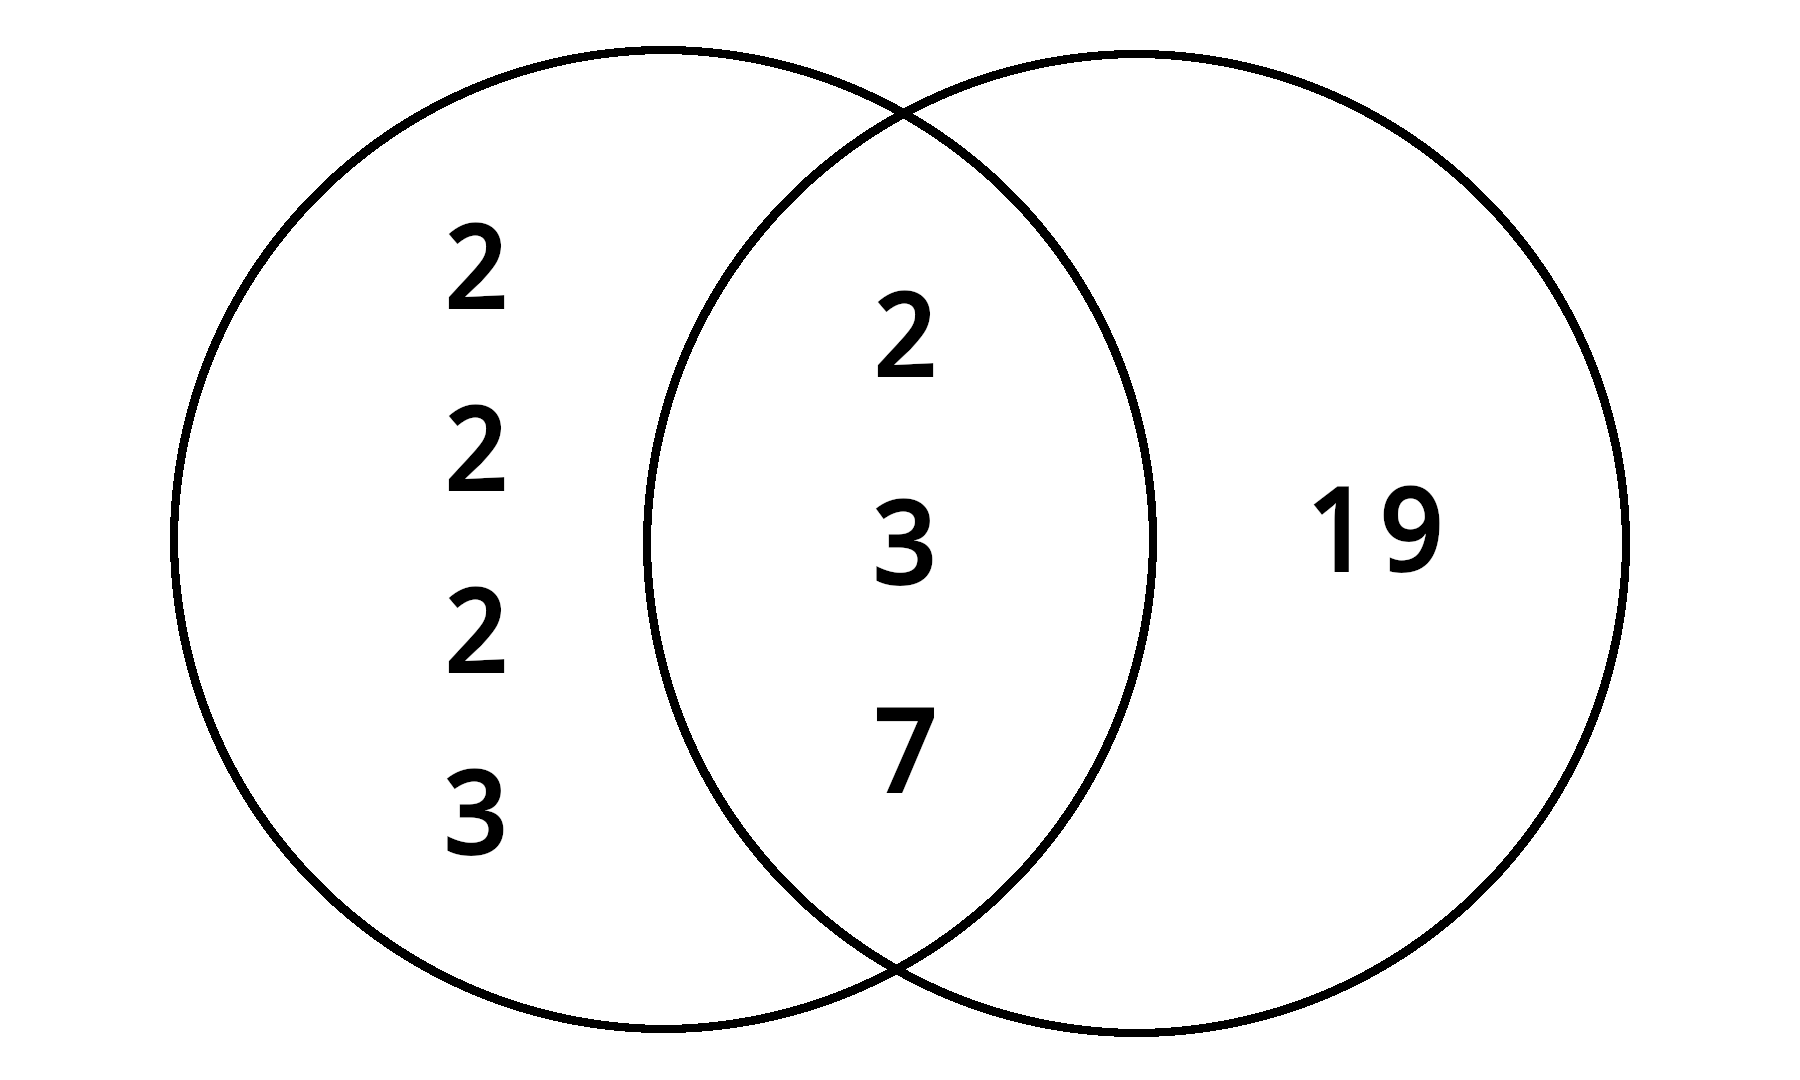
\includegraphics{viete-lcd.png}

\textit{Więc:}\\
$$\text{NNW}(798, 1008) = 2^{4} \cdot 3^{2} \cdot 7 \cdot 19 = 19152$$
$$\text{NWD}(798, 1008) = 2 \cdot 3 \cdot 7 = 42$$\hfill\break

\noindent\subsection{Oprocentowanie lokat i kredytów}

\noindent\textbf{Procent prosty}
 - rodzaj oprocentowania polegający na tym, że odsetki doliczane do wkładu nie podlegają oprocentowaniu.\hfill\break
\noindent\textbf{Procent składany}
 - rodzaj oprocentowania, który nalicza procent od odsetek doliczonych do wkładu w każdym kolejnym rozpatrywanym okresie.\hfill\break
 Doliczanie odsetek do lokaty nazywa się \textbf{kapitalizacją odsetek}, a czas między kapitalizacjami \textbf{okresem kapitalizacji}.\hfill\break\\

\noindent Niech $K_{0}$ będzie początkowym wkładem pieniężnym, $K$ - końcową otrzymaną kwotą, $n$ - liczbą równych okresów kapitalizacji, które miały miejsce w okresie $m$, $m$ - liczbą okresów oszczędzania, $r$ - stopą oprocentowania, $p$ - podatkiem od dochodów kapitałowych.
Wtedy:



\renewcommand{\arraystretch}{2}
\setlength{\arrayrulewidth}{0.5mm}

\begin{equation*}
   \begin{array}{lc}
      \textbf{Procent prosty:} & K = K_{0}\cdot\left(1+\dfrac{r}{n}\right)^{n\cdot m}\\
      \textbf{Procent składany:} & K = K_{0}\cdot\left[ 1+\dfrac{r}{n}\left(1 - \dfrac{p}{100}\right)\right]^{n\cdot m}
   \end{array}
\end{equation*}

\newpage

\section{Wielomiany, funkcje wielomianowe}
\subsection{Informacje i twierdzenia}
\textbf{Wielomianem stopnia \textit{n}, \textit{n} $\in \mathbb{N}_{+}$ zmiennej rzeczywistej x} nazywamy wyrażenie:
$$W(x) = a_{n}x^{n}+a_{n-1}x^{n-1}+a_{n-2}x^{n-2}+\ldots+a_{2}x^{2}+a_{1}x+a_{0},$$
gdzie $a_{0}, a_{1}, a_{2}, \ldots, a_{n} \in \mathbb{R} \land a_{n} \neq 0$. Liczby $a_{0}, a_{1}, a_{2}, \ldots, a_{n}$ to współczynniki wielomianu.
Wielomian stopnia zerowego to każda liczba rzeczywista różna od zera. Wielomian zerowy to liczba równa zeru; nie ma określonego stopnia.\\
\smallskip

\noindent\textbf{Wielomian W(\textit{x}) jest podzielny przez wielomian P(\textit{x})} rózny od wielomianu zerowego wtedy i tylko wtedy,
gdy istnieje taki wielomian Q(\textit{x}), dla którego prawdziwa jest równość:
$$W(x) = P(x) \cdot Q(x)$$
Wówczas Q(\textit{x}) nazywany jest ilorazem wielomianu W(\textit{x}) przez P(\textit{x}), a P(\textit{x}) 
jest dzielnikiem wielomianu W(\textit{x}).\\

\smallskip
\noindent\textbf{Pierwiastek wielomianu W(\textit{x})} to liczba rzeczywista $a$, dla której $W(a) = 0$.\\

\smallskip
\noindent\textbf{Pierwiastek \textit{k}-krotny wielomianu W(\textit{x})}, gdzie $k \in \mathbb{N}_{+}$ to liczba $a$ taka, że W(\textit{x})
jest podzielny przez $(x-a)^{k}$ i nie jest podzielny przez $(x-a)^{k+1}$. Liczba $k$ jest nazywana krotnością pierwiastka.\\

\bigskip

\noindent\textbf{Twierdzenie o dzieleniu (rozkładzie) wielomianu}\\
Jeśli W(\textit{x}) oraz P(\textit{x}) są wielomianami i P(\textit{x}) nie jest wielomianem zerowym, 
to istnieją dwa wielomiany Q(\textit{x}) oraz R(\textit{x}) takie, że prawdziwa jest równość:
$$W(x) = P(x)\cdot Q(\textit{x})+R(x),$$
gdzie R(\textit{x}) jest wielomianem zerowym lub wielomianem o stopniu mniejszym od stopnia wielomianu P(\textit{x}).\\

\smallskip
\noindent\textbf{Twierdzenie o reszcie wielomianu}\\
Reszta z dzielenia wielomianu W(\textit{x}) przez dwumian $(x - a)$ jest równa W(\textit{a}).\\

\smallskip
\newpage
\noindent\textbf{Twierdzenie o wymiernych pierwiastkach wielomianu o współczynnikach całkowitych}\\
Jeżeli wielomian W(\textit{x}) ma pierwiastek wymierny, który można zapisać w postaci nieskracalnego ułamka $\frac{p}{q}$, gdzie $p, q \in \mathbb{C} \land q \neq 0$, to 
$p$ jest dzielnikiem wyrazu wolnego $a_{0}$, natomiast $q$ - dzielnikiem współczynnika $a_{n}$ przy najwyższej potędze zmiennej.\\

\smallskip
\noindent\textbf{Twierdzenie B\'ezouta}\\
Liczba $a$ jest pierwiastkiem wielomianu W(\textit{x}) wtedy i tylko wtedy, gdy wielomian W(\textit{x}) jest podzielny bez reszty przez dwumian $(x - a)$.\\

\smallskip
\noindent\textbf{Twierdzenie o liczbie pierwiastków wielomianu}\\
Każdy wielomian stopnia $n$ ma co najwyżej $n$ pierwiastków.\\

\smallskip
\noindent\textbf{Twierdzenie o rozkładzie wielomianu na czynniki}\\
Każdy wielomian stopnia co najmniej trzeciego można rozłożyć na czynniki sponia co najwyżej drugiego.
Rozkład w taki sposób jest jednoznaczny (z dokładnością co do kolejności czynników i stałej).\\

\smallskip
\noindent\textbf{Reguła znaków Kartezjusza}\\
Dla dowolnego wielomianu o rzeczywistych współczynnikach, uporządkowanych według malejącej potęgi zmiennej,
ilość dodatnich miejsc zerowych wielomianu jest równa liczbie zmian znaków między niezerowymi współczynnikami, 
albo jest mniejsza o wielokrotność liczby 2.\\

\smallskip

\renewcommand{\arraycolsep}{0.35cm}
\renewcommand{\arraystretch}{1.25}

\noindent\textbf{Schemat Hornera}\\
Sposób oblicznia wartości wielomianu dla danej wartości argumentu. Wykorzystywany również do przeprowadzania
dzielenia wielomianu przez dwumian w formie $(x - a),\;a \in \mathbb{R}$ na podstawie twierdzenia B\'ezouta.\hfill\break\\
\textit{Przykład:}
$$\text{Podziel } \;W(x) = x^{4}-22x^{2}-56x+77\; \text{ przez dwumian }\; x - 1$$
\textit{1. Zapisz wszystkie współczynniki wielomianu od najwyższej potęgi (także z zerowymi)
oraz $a$ z dwumianu. Przepisz pierwszy współczynnik do najniższej linijki:}\\
\begin{center}
$\begin{array}{c|ccccc}
    & 1 & 0 & -22 & -56 & 77\\
  1 & \downarrow   &   &     &     &   \\ \hline
    & 1  &   &     &\multicolumn{1}{c|}{}   &
\end{array}$\end{center}

\noindent\textit{2. Pomnóż przeniesiony współczynnik przez $a$ zapisane po lewej stronie:}\\
\begin{center}
$\begin{array}{c|ccccc}
   & 1 & 0 & -22 & -56 & 77\\
 1 &   & 1 \cdot 1  &     &     &   \\ \hline
   & 1  &   &     &\multicolumn{1}{c|}{}   &
\end{array}$\end{center}

\noindent\textit{3. Dodaj ze sobą współczynnik z górnego wiersza do właśnie policzonego iloczynu poniżej:}\\
\begin{center}
   $\begin{array}{c|ccccc}
      & 1 & 0 & -22 & -56 & 77\\
    1 &   & 1 &     &     &   \\ \hline
      & 1 & 0 + 1  &     &\multicolumn{1}{c|}{}   &
   \end{array}$\end{center}

\noindent\textit{4. Powtarzaj operacje mnożenia i dodawania aż do ostatniej kolumny:}\\
\begin{center}
   $\begin{array}{c|ccccc}
      & 1 & 0 & -22 & -56 & 77\\
    1 &   & 1 &  1\cdot 1   & -21 \cdot 1 & -77\cdot 1  \\ \hline
      & 1 & 1 &  -22 + 1   &\multicolumn{1}{c|}{-56 + (-21) }  & 77 + (-77)
   \end{array}$
\end{center}

\noindent\textit{Otrzymujemy tabelkę wypełnioną w następujący sposób:}\\
\begin{center}
   $\begin{array}{c|ccccc}
      & 1 & 0 & -22 & -56 & 77\\
    1 &   & 1 &  1   & -21 & -77\\ \hline
      & \textcolor{NavyBlue}{1} & \textcolor{NavyBlue}{1} &  \textcolor{NavyBlue}{-21}   &\multicolumn{1}{c|}{\textcolor{NavyBlue}{-77} }  & \textbf{\textcolor{RawSienna}{0}}
   \end{array}$
\end{center}

\noindent\textit{Więc:}\\
$$\underbrace{(x^{4}-22x^{2}-56x+77)}_{W(x)} = \underbrace{(x - 1)}_{P(x)}\underbrace{(\textcolor{NavyBlue}{1}x^{3} + \textcolor{NavyBlue}{1}x^{2} \textcolor{NavyBlue}{- 21}x \textcolor{NavyBlue}{- 77})}_{\text{Q(x)}} + \underbrace{\textcolor{RawSienna}{0}}_{\text{R(x)}} \Leftrightarrow W(1) = 0$$

\subsection{Funkcja liniowa}
\noindent\textbf{Wzór ogólny:}
$$f(x) = ax + b;\;\; a, b \in \mathbb{R}$$
Liczba $a$ nazywana jest współczynnikiem kierunkowym, $b$ wyrazem wolnym. Dziedziną i zbiorem wartości
funkcji liniowej są liczby rzeczywiste.\hfill\break
\vspace{1pt}

\noindent Funkcja liniowa przecina oś OY w punkcie $(0, b)$, a oś OX w $(-\frac{b}{a}, 0)$. Wykres funkcji liniowej 
jest nachylony do osi OX pod kątem $\alpha$ takim, że $\text{tg}\;\alpha = a$.\\

\noindent Funkcja liniowa jest:
\begin{itemize}
   \item nieograniczona,
   \item nieokresowa,
   \item monotoniczna ($a > 0 \text{ - rosnąca}, a < 0 \text{ - malejąca}, a = 0 \text{ - stała}$),
   \item różnowartościowa (gdy $a \neq 0$),
   \item ciągła,
   \item różniczkowalna: $f^{\prime}(x) = a$.
\end{itemize}

\subsection{Funkcja kwadratowa}
\noindent\textbf{Wzór w postaci ogólnej:}
$$f(x) = ax^{2} + bx + c;\;\; a, b, c \in \mathbb{R}, a \neq 0$$
\noindent\textbf{Wzór w postaci kanonicznej:}
$$f(x) = a(x - p)^{2} + q;\;\; p = -\frac{b}{2a},\;\; q = -\frac{\Delta}{4a}, \;\; \Delta = b^{2} -4ac$$
\noindent\textbf{Wzór w postaci iloczynowej:}
$$f(x) = a(x - x_{1})(x - x_{2}) \Leftrightarrow \Delta \geq 0; \;\; x_{1} = \frac{-b + \sqrt{\Delta}}{2a},\;\; x_{2} = \frac{-b - \sqrt{\Delta}}{2a}$$

\noindent\textbf{Delta, wyróżnik wielomianu stopnia drugiego} - Liczba opisująca relację między współczynnikami funkcji 
kwadratowej a jej miejscami zerowymi. Wyznaczona wzorem $\Delta_{2} = b^{2} - 4ac$.
\begin{itemize}
   \item $\Delta > 0$ - Dwa różne pierwiastki rzeczywiste: $x_{1}, x_{2} = \frac{-b \pm\sqrt{\Delta}}{2a}$,
   \item $\Delta = 0$ - Jeden pierwiastek rzeczywisty podwójny: $x_{0} = -\frac{b}{2a}$,
   \item $\Delta < 0$ - Brak pierwiastków rzeczywistych: ($x_{1}, x_{2} \in \mathbb{C}$\;(zespolonych)).
\end{itemize}

\noindent Wykresem funkcji kwadratowej jest parabola, której ramiona skierowane są do góry gdy $a > 0$ a do dołu,
gdy $a < 0$.\hfill\break


\noindent\textbf{Wierzchołek funkcji kwadratowej} znajduje się w punkcie $\left(-\frac{b}{2a}, -\frac{\Delta}{4a}\right)$.
Alternatywnie, współrzędną \textbf{x} wierzchołka można wyliczyć średnią arytmetyczną miejsc zerowych: $p = \frac{x_{1} + x_{2}}{2}$, a 
współrzędną \textbf{y} wartością funkcji w punkcie $p$: $q = f(p)$.\hfill\break

\noindent\textbf{Wzory Viète'a} - wzory wiążące współczynniki wielomianu (stopnia drugiego) z jego pierwiastkami:\hfill\break
\begin{equation*}
   \left\{
      \begin{array}{ll}
         \!\!\!\!x_{1} + x_{2} = -\frac{\displaystyle b}{\displaystyle a}\\
         \!\!\!\!x_{1}\cdot x_{2} = \frac{\displaystyle c}{\displaystyle a}\\
      \end{array}
   \right.
   \end{equation*}

\noindent Dziedziną funkcji kwadratowej jest zbiór liczb rzeczywistych. Zbiorem wartości jest przedział
$\langle q, +\infty) \text{ dla } a > 0$, $(-\infty, q\rangle \text{ dla } a < 0$.\hfill\break

\noindent Funkcja kwadratowa jest:
\begin{itemize}
   \item nieokresowa,
   \item monotoniczna w przedziałach:
   $$\text{malejąca w }(-\infty, p\rangle, \text{ rosnąca w } \langle p, +\infty),\;\; a > 0$$
   $$\text{rosnąca w }(-\infty, p\rangle, \text{ malejąca w } \langle p, +\infty),\;\; a < 0$$
   \item ciągła,
   \item różniczkowalna: $f^{\prime}(x) = 2ax + b$,
   \item ściśle wypukła dla $a > 0$, ściśle wklęsła dla $a < 0$.

\end{itemize}

\subsection{Funkcja sześcienna}
\noindent\textbf{Wzór w postaci ogólnej:}
$$f(x) = ax^{3} + bx^{2} + cx + d;\;\; a, b, c, d \in \mathbb{R}, a \neq 0$$
\noindent\textbf{Wzór w postaci kanonicznej:}
$$f(t) = t^{3} + pt + q;\;\; t = x + \frac{b}{3a}, \;\;p = \frac{c}{a}-\frac{b^{2}}{3a^{2}},\;\; q = \frac{2b^{3}}{27a^{3}}+\frac{d}{a}-\frac{bc}{3a^{2}}$$
\noindent\textbf{Wzór w postaci iloczynowej:}
$$f(x) = a(x - x_{1})(x - x_{2})(x - x_{3})$$
\noindent\textbf{Wyróżnik wielomianu stopnia trzeciego} - Liczba opisująca relację między współczynnikami funkcji 
sześciennej a jej miejscami zerowymi. Wyznaczona wzorem $\Delta_{3} = b^{2}c^{2} - 4ac^{3} - 4b^{3}d + 18abcd - 27a^{2}d^{2}$.


\begin{itemize}
   \item $\Delta_{3} > 0$ - Trzy różne pierwiastki rzeczywiste: $x_{1}, x_{2}, x_{3}$,
   \item $\Delta_{3} = 0$ - Dwa różne pierwiastki rzeczywiste, z czego jeden dwukrotny lub jeden pierwiastek trzykrotny,
   \item $\Delta_{3} < 0$ - Jeden pierwiastek rzeczywisty, dwa pozostałe w liczbach zespolonych.
\end{itemize}

\noindent\textbf{Ekstrema funkcji sześciennej} (punkty krytyczne) znajdują się w punktach $(p, f(p))$, gdzie $p$ wyznaczone
jest wzorem: $p = \frac{-b \pm \sqrt{b^{2} - 3ac}}{3a}$. Jeżeli $b^{2} - 3ac$ jest
mniejsze bądź równe 0, wtedy ekstrem nie ma (funkcja $f(x)$ jest monotoniczna w całej dziedzinie).\hfill\break

\noindent\textbf{Środek symetrii funkcji sześciennej} (punkt przegięcia) znajduje się w punkcie o współrzędnych 
$\left(-\frac{b}{3a}, \;\frac{2b^{3}}{27a^{2}} - \frac{bc}{3a} + d\right)$.\hfill\break

\noindent\textbf{Wzory Viète'a} - wzory wiążące współczynniki wielomianu (stopnia trzeciego) z jego pierwiastkami:\hfill\break
\begin{equation*}
   \left\{
      \begin{array}{ll}
         \!\!\!\!x_{1} + x_{2} + x_{3} = -\frac{\displaystyle b}{\displaystyle a}\\
         \!\!\!\!x_{1}x_{2} + x_{1}x_{3} + x_{2}x_{3} = \frac{\displaystyle c}{\displaystyle a}\\
         \!\!\!\!x_{1}x_{2}x_{3} = -\frac{\displaystyle d}{\displaystyle a}\\
      \end{array}
   \right.
\end{equation*}\hfill\break

\noindent Dziedziną i zbiorem wartości funkcji sześciennej jest zbiór liczb rzeczywistych.\hfill\break

\noindent Funkcja sześcienna jest:
\begin{itemize}
   \item nieokresowa,
   \item monotoniczna w przedziałach:
\begin{itemize}
   \item $\text{rosnąca w }(-\infty, p_{1}\rangle\text{ i }\langle p_{2}, +\infty), \text{ malejąca w } \langle p_{1}, p_{2}\rangle,$\\ $ a > 0, \;\;b^{2} - 3ac > 0$
   \item $\text{malejąca w }(-\infty, p_{1}\rangle\text{ i }\langle p_{2}, +\infty), \text{ rosnąca w } \langle p_{1}, p_{2}\rangle,$\\ $ a < 0, \;\;b^{2} - 3ac > 0$
   \item $\text{rosnąca w całej dziedzinie}, \;\;a > 0, \;\;b^{2} - 3ac \leq 0$
   \item $\text{malejąca w całej dziedzinie}, \;\;a < 0, \;\;b^{2} - 3ac \leq 0$
\end{itemize}

   \item ciągła,
   \item różniczkowalna: $f^{\prime}(x) = 3ax^{2} + 2bx + c$,
   \item ściśle wypukła w przedziale:
   $$\left(-\frac{b}{3a}, +\infty\right) \text{ dla a > 0}, \left(-\infty, -\frac{b}{3a}\right) \text{ dla a < 0}$$
   \item ściśle wklęsła w przedziale:
   $$\left(-\infty, -\frac{b}{3a}\right) \text{ dla a > 0}, \left(-\frac{b}{3a}, +\infty\right) \text{ dla a < 0}$$

\end{itemize}

\subsection{Funkcja wymierna}
Funkcja będąca ilorazem funkcji wielomianowych. 
Iloraz wielomianów realizujących dane funkcje wielomianowe nazywa się wyrażeniem wymiernym.
\noindent\textbf{Wzór w postaci ogólnej:}
$$f(x) = \frac{P(x)}{Q(x)};\;\;P(x), Q(x) - \text{wielomiany}, \;Q(x) \not\equiv 0$$

\noindent\textbf{Asymptoty funkcji wymiernej}
\begin{itemize}
   \item Pionowa:\hfill\break
   Wszystkie miejsca, gdzie mianownik funkcji wymiernej $Q(x) = 0$.
   \item Pozioma:\hfill\break
   Niech $L$ będzie stopniem licznika funkcji wymiernej, $M$ stopniem mianownika funkcji wymiernej, a $a_{L}, a_{M}$ to kolejno
   współczynniki przy największej potędze licznika i mianownika.
   Wtedy:\hfill\break
   \begin{equation*}      
   \begin{array}{c|c|c}
      L < M & L = M & L > M\\
      \hline
      y = 0 & y = \frac{\displaystyle a_{L}}{\displaystyle a_{M}} & \text{Brak asymptoty poziomej}\\
   \end{array}
   \end{equation*}
   \item Ukośna:\hfill\break
   Występuje, gdy stopień licznika jest o jeden większy od mianownika.
   Aby policzyć wzór jej prostej należy przeprowadzić pisemne dzielenie licznika przez mianownik.
   Wynikiem jest iloraz dzielenia.

   \newpage
\textit{Przykład:}
$$f(x) = \frac{2x^{3}-4x^{2}+6x+9}{2x^{2}-10x+4}$$\hfill\break
\textit{Stopień licznika jest o 1 większy od mianownika, więc:}
   \begin{center}
   \polyset{style=A}
   \polylongdiv{2x^3-4x^2+6x+9}{2x^2-10x+4}
   \end{center}\hfill\break
$$2x^{3}-4x^{2}+6x+9 = \textcolor{OliveGreen}{\underline{(x+3)}}(2x^{2}-10x+4)+32x - 3$$
$$\text{Asymptota ukośna: }y = x + 3$$

\end{itemize}\hfill\break
\smallskip

\noindent Specjalnym przypadkiem funkcji wymiernej jest \textbf{funkcja homograficzna}.\hfill\break
\textbf{Wzór w postaci ogólnej:}
$$f(x) = \frac{ax + b}{cx + d};\;\;a, b, c, d \in \mathbb{R},\;c\neq 0,\; ad - bc \neq 0$$
   
\noindent Dziedziną funkcji homograficznej jest zbiór liczb rzeczywistych z wyłączeniem jednego miejsca zerowego
opisanego wzorem $-\frac{d}{c}$.\hfill\break\\
 Zbiór wartości to zbiór liczb rzeczywistych z wyłączeniem punktu $\frac{a}{c}$,
którego zawarcie sprawiłoby, że funkcja homograficzna spełniałaby równanie $ad - bc = 0$.\hfill\break\\
Asymptota pionowa opisana jest równaniem $x = -\frac{d}{c}$, a asymptota pozioma $y = \frac{a}{c}$.\hfill\break\\
Środkiem symetrii a zarazem punktem przecięcia asymptot jest punkt o współrzędnych $S = \left(-\frac{d}{c}, \frac{a}{c}\right)$.\hfill\break\\
Funkcja homograficzna jest monotoniczna w przedziałach $\left(-\infty, -\frac{d}{c}\right) \text{ i } \left(-\frac{d}{c}, +\infty\right)$.
Jest przedziałami rosnąca, gdy $ad - bc > 0$ a przedziałami malejąca, gdy $ad - bc < 0$.
\newpage









   
   
   

\noindent\section{Właściwości i wykresy funkcji}
\noindent\textbf{Funkcja} - relacja między elementami zbioru $X$ i $Y$ taka, że każdemu elementowi
zbioru $X$ przyporządkowany jest dokładnie jeden element zbioru $Y$.

$$f:X \rightarrow Y$$
\includegraphics{funkcja zbiór.png}\hfill\break

\noindent \textit{Funkcja $f$ przedstawiona jako graf. Każdemu argumentowi ze zbioru $X$ przyporządkowano dokładnie jeden element ze zbioru $Y$. 
Dwóm różnym elementom w zbiorze $X$ może odpowiadać ten sam element $Y$. Nie każdy element zbioru $Y$ musi być wartością funkcji $f$.}\hfill\break\\
\noindent Zbiór $X$ nazywa się dziedziną lub zbiorem argumentów, a zbiór $Y$ - przeciwdziedziną lub zbiorem wartości.\\
Każdy $x \in X$ to argument funkcji $f$, a $y \in \{n: n \in Y \land n = f(x)\}$ - wartością funkcji.\\
Funkcja $f$ to przekształcenie (odwzorowanie) zbioru $X$ w zbiór $Y$.\hfill\break\\

\noindent\textbf{Twierdzenie Darboux} - Niech funkcja $f(x)$ będzie funkcją ciągłą, a na jej dziedzinie
niech będzie zdefiniowany przedział domknięty $\langle a, b\rangle $. Wtedy, jeżeli $f(a) > f(c) > f(b)$ lub
$f(a) < f(c) < f(b)$ to punkt $c \in \langle a, b\rangle$. Szczególnym przypadkiem jest, gdy $a$ i $b$ mają różne
znaki. Wtedy w przedziale domkniętym między nimi gwarantowane jest istnienie c takiego, że $f(c) = 0$.

\subsection{Właściwości funkcji}
\begin{itemize}
   \item Różnowartościowa (iniekcja)\hfill\break
      Funkcja dla każdego elementu dziedziny przyjmuje różny element z przeciwdziedziny co najwyżej raz:
      $$f:X \rightarrow Y \text{ - różnowartościowa } \Leftrightarrow \underset{a, b \in X}{\bigwedge} a \neq b \Rightarrow f(a) \neq f(b)$$
   \item Funkcja ''na'' (suriekcja)\hfill\break
      Funkcja, która przyjmuje wszystkie wartości z przeciwdziedziny:
      $$f:X \rightarrow Y \text{ - ''na'' } \Leftrightarrow \underset{y \in Y}{\bigwedge} \underset{x \in X}{\bigvee} f(x) = y$$
   \item Funkcja wzajemnie jednoznaczna (bijekcja)\hfill\break
      Funkcja, w którek każdemu elementowi dziedziny odpowiada jeden i tylko jeden element z przeciwdziedziny,
      przy czym każdy $y$ należący do zbioru $Y$ jest obrazem zbioru $X$.
      Funkcja wzajemnie jednoznaczna jest jednocześnie różnowartościowa i ''na''.
   \item Addytywna\hfill\break
      Funkcja zachowuje operację dodawania: $f(x + y) = f(x) + f(y)$
   \item Multiplikatywna\hfill\break
      Funkcja zachowuje operację mnożenia: $f(xy) = f(x)f(y)$
   \item Parzysta\hfill\break
      Wykres funkcji jest symetryczny względem osi rzędnych (OY): $f(x) = f(-x)$
   \item Nieparzysta\hfill\break
      Wykres funkcji jest symetryczny wzglęgem środka układu współrzędnych: $f(x) = -f(x)$
   \item Ciągła\hfill\break
      Arbitralnie mała zmiana wartości funkcji jest uzasadniona arbitralnie małą zmianą argumentu funkcji.
      Pozbawiona jest też punktów nieciągłości pierwszego rodzaju usuwalnych, pierwszego rodzaju i drugiego rodzaju.
   \item Monotoniczna\hfill\break
      Funkcja, która zachowuje pewien określony porządek zbiorów. Niech $f:X\rightarrow Y$ będzie
      dowolną funkcją na uporządkowanych zbiorach $X, Y$, a $x_{1}, x_{2}$ elementami dziedziny funkcji $f$.
      Wówczas funkcja $f$ jest:
      \begin{itemize}
         \item rosnąca (silnie rosnąca), gdy $x_{1} < x_{2} \Rightarrow f(x_{1}) < f(x_{2})$
         \item malejąca (silnie malejąca), gdy $x_{1} < x_{2} \Rightarrow f(x_{1}) > f(x_{2})$
         \item nierosnąca (słabo rosnąca), gdy $x_{1} < x_{2} \Rightarrow f(x_{1}) \leq f(x_{2})$
         \item niemalejąca (słabo malejąca), gdy $x_{1} < x_{2} \Rightarrow f(x_{1}) \geq f(x_{2})$
         \item stała, gdy dla dowolnych $x_{1}, x_{2} \in X \Rightarrow f(x_{1}) = f(x_{2})$
      \end{itemize}
   \item Różniczkowalna\hfill\break
      Funkcja ma pochodną w każdym punkcie swojej dziedziny, oraz wartość tej pochodnej jest skończona.
   \item Okresowa\hfill\break
      Funkcja jest okresowa, gdy pewne wartości pojawiają się cyklicznie co pewien regularny odstęp.
      Niech $C, \;C \neq 0$ będzie pewną stałą wartością (okresem funkcji). Wtedy dla funkcji okresowej prawdziwa jest równość:
      $$f(x + C) = f(x)$$
   \item Wypukła\hfill\break
      Wykres funkcji $f$ w przedziale $(a, b)$ leży ponad prostą wyznaczoną przez pochodną w punkcie $x_{0} \in (a, b)$
   \item Wklęsła\hfill\break
      Wykres funkcji $f$ w przedziale $(a, b)$ leży pod prostą wyznaczoną przez pochodną w punkcie $x_{0} \in (a, b)$
\end{itemize}

\subsection{Wykresy funkcji}
{%
\setlength{\fboxsep}{0pt}%
\setlength{\fboxrule}{0.5pt}%


\begin{center}
\begin{tabular}{cc}
   \fbox{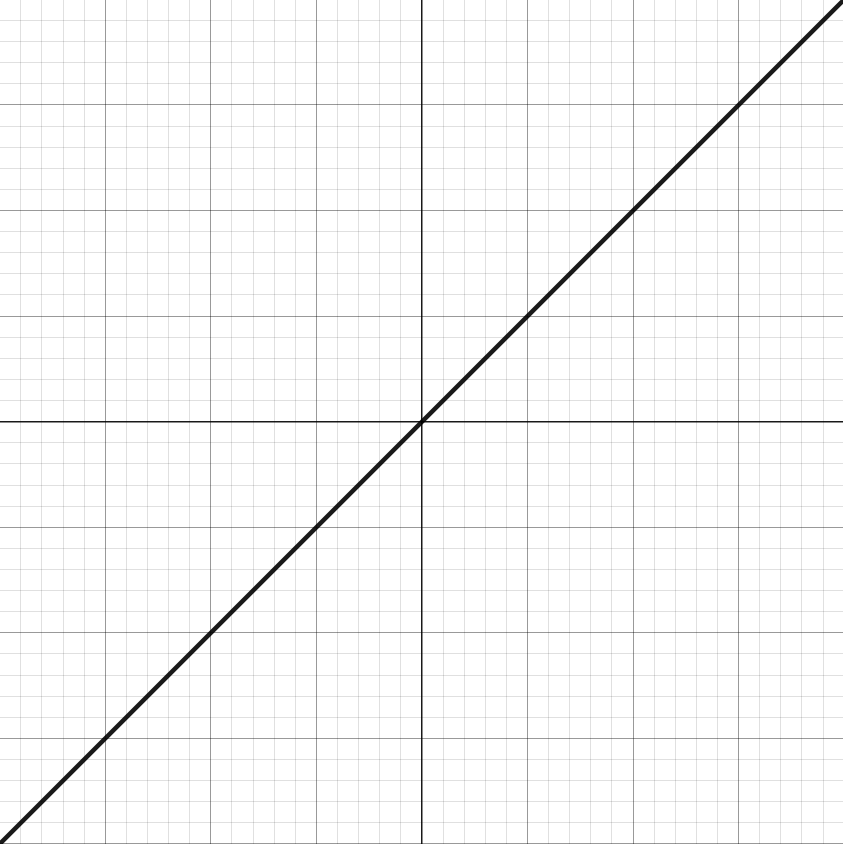
\includegraphics[scale=0.3]{liniowa.png}} & \fbox{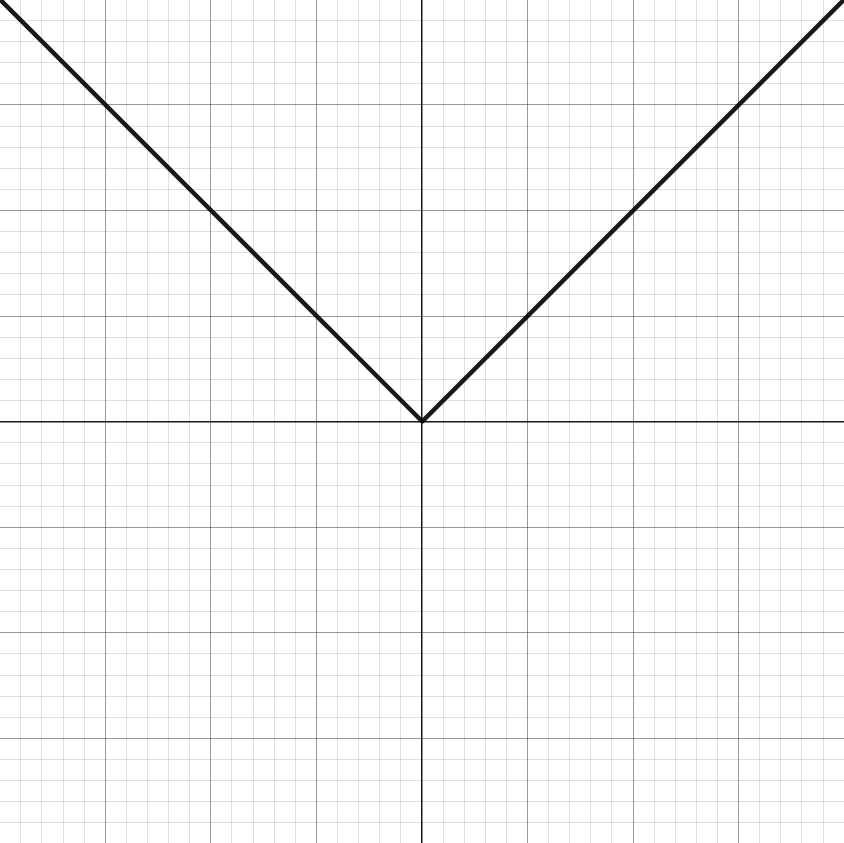
\includegraphics[scale=0.3]{bezwzględna.png}}\\
   $f(x) = x$ & $f(x) = \vert x \vert$
\end{tabular}

\begin{tabular}{cc}
   \fbox{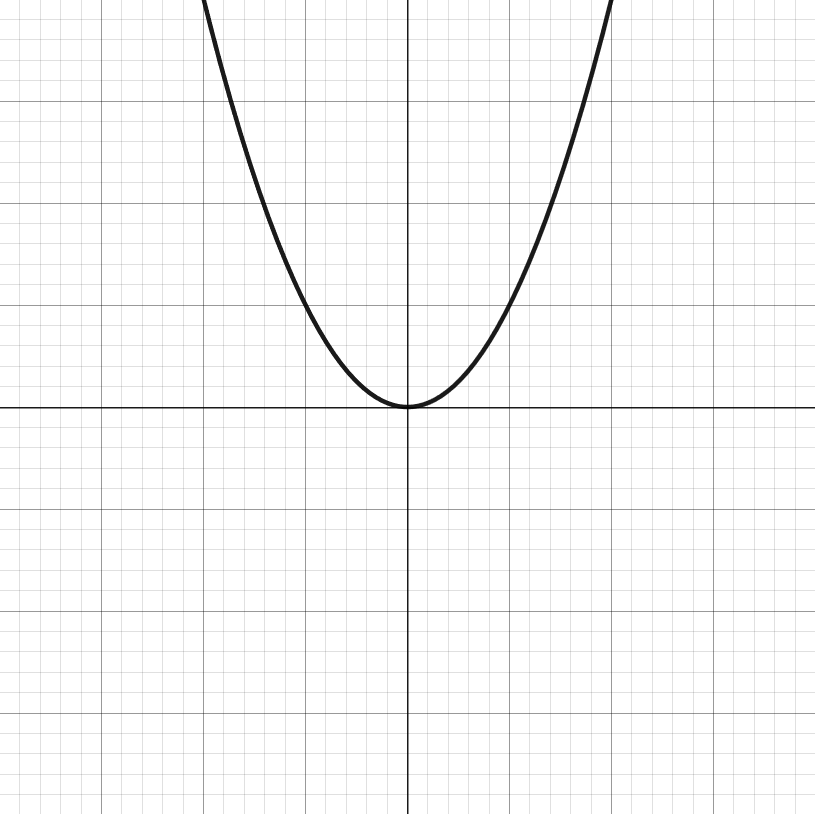
\includegraphics[scale=0.318]{kwadratowa.png}} & \fbox{\includegraphics[scale=0.318]{sześcienna.png}}\\
   $f(x) = x^{2}\text{ - }\textbf{parabola} $ & $f(x) = x^{3}$
\end{tabular}

\begin{tabular}{cc}
   \fbox{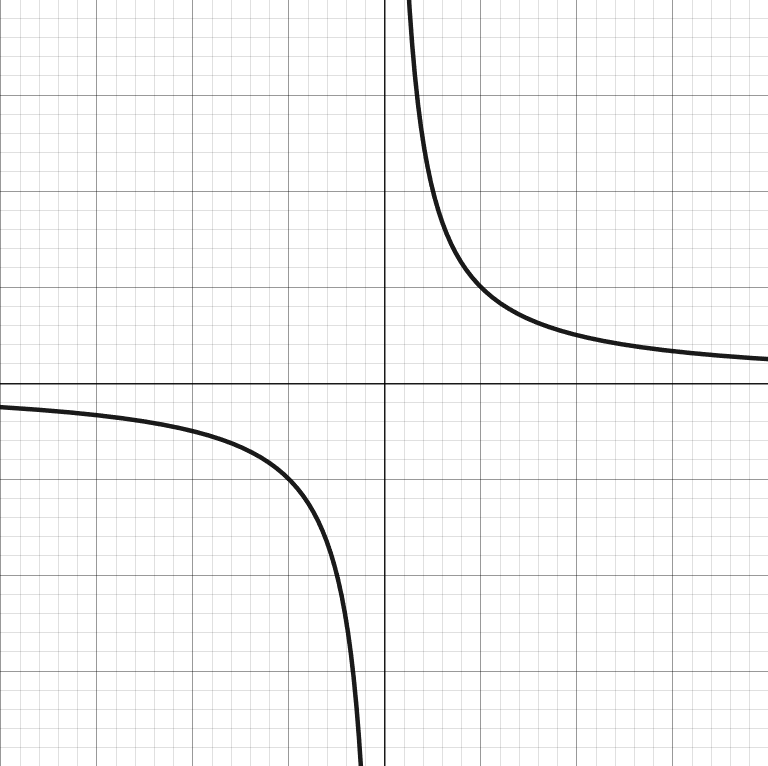
\includegraphics[scale=0.338]{hiperboliczna.png}} & \fbox{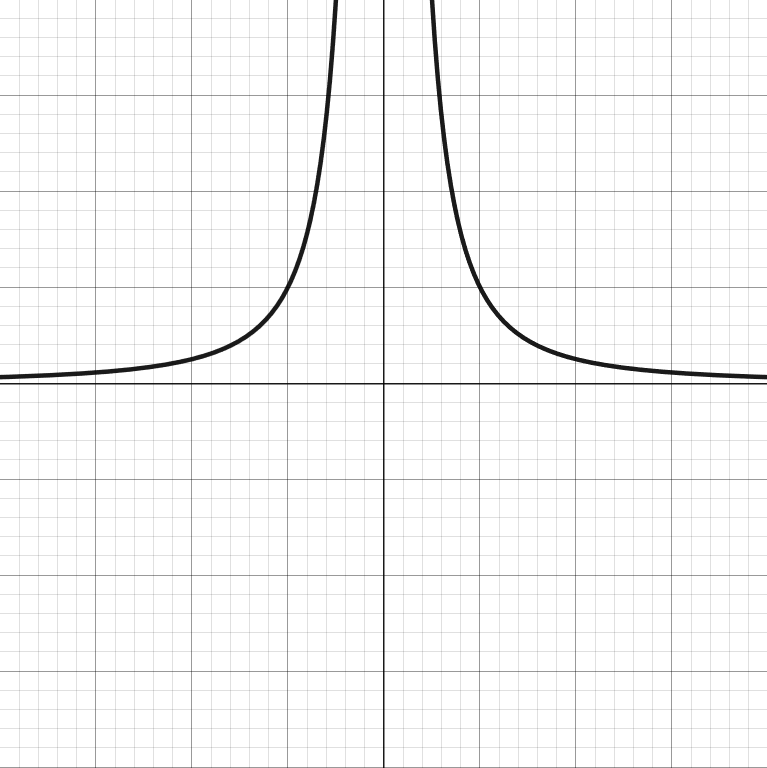
\includegraphics[scale=0.338]{hiperboliczna kwadrat.png}}\\
   $f(x) = \dfrac{1}{x}\text{ - }\textbf{hiperbola}$ & $f(x) = \dfrac{1}{x^{2}} $
\end{tabular}

\begin{tabular}{cc}
   \fbox{\includegraphics[scale=0.318]{wykładnicza.png}} & \fbox{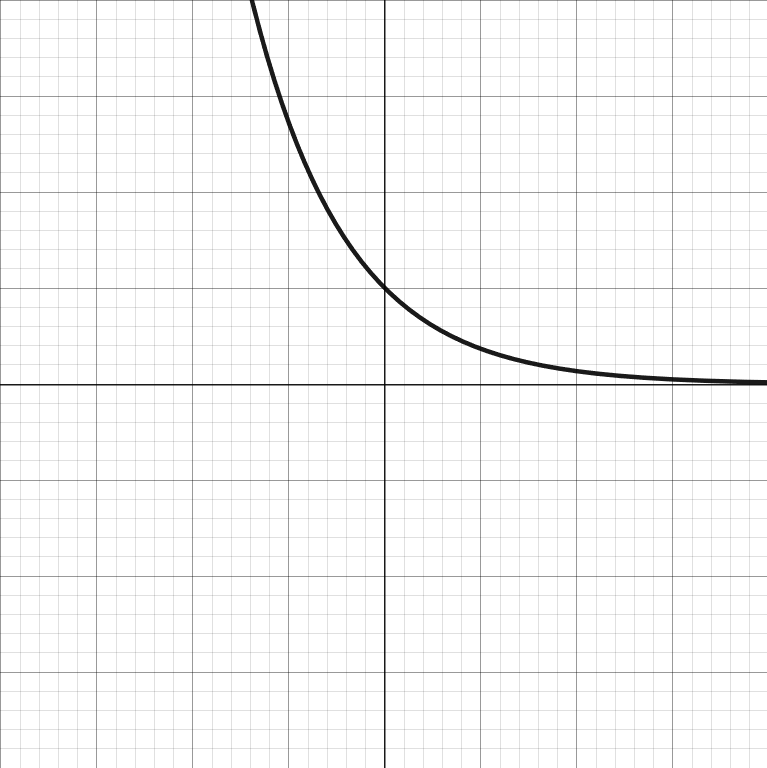
\includegraphics[scale=0.338]{wykładnicza potęga ujemna.png}}\\
   $f(x) = a^{x}, \;a > 1$ & $f(x) = a^{x}, \;0 < a < 1$
\end{tabular}

\begin{tabular}{cc}
   \fbox{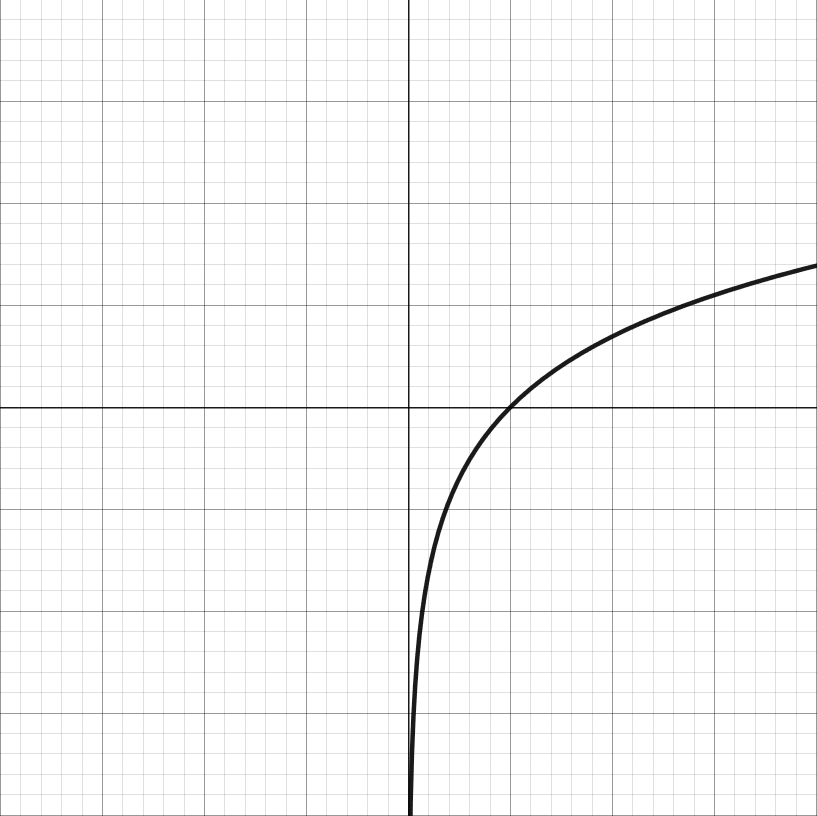
\includegraphics[scale=0.318]{logarytmiczna.png}} & \fbox{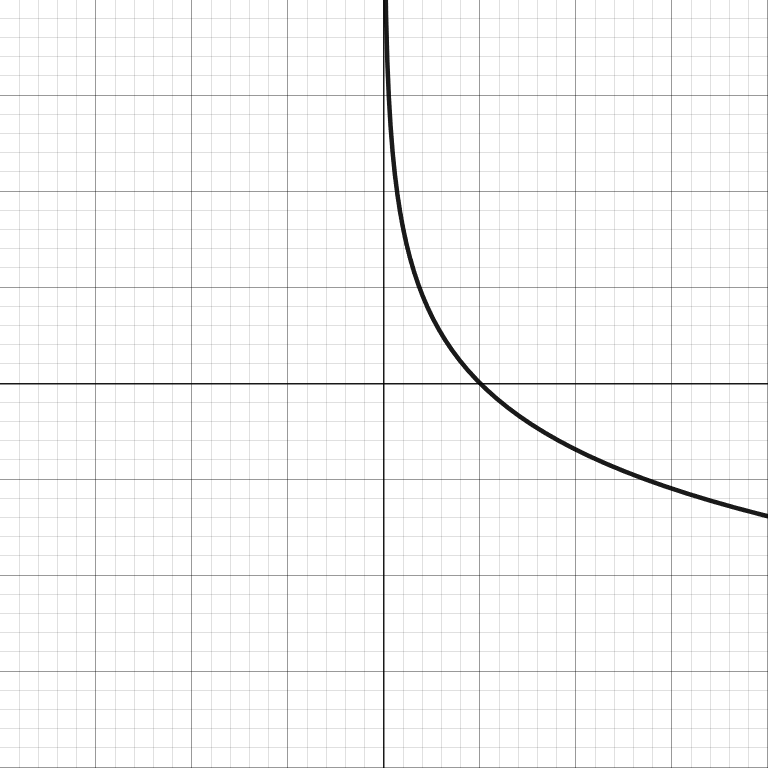
\includegraphics[scale=0.337]{logarytmiczna 1 nad x.png}}\\
   $f(x) = \log_{a}x,\;a > 1$ & $f(x) = \log_{a}x,\;0 < a < 1$
\end{tabular}

\begin{tabular}{cc}
   \fbox{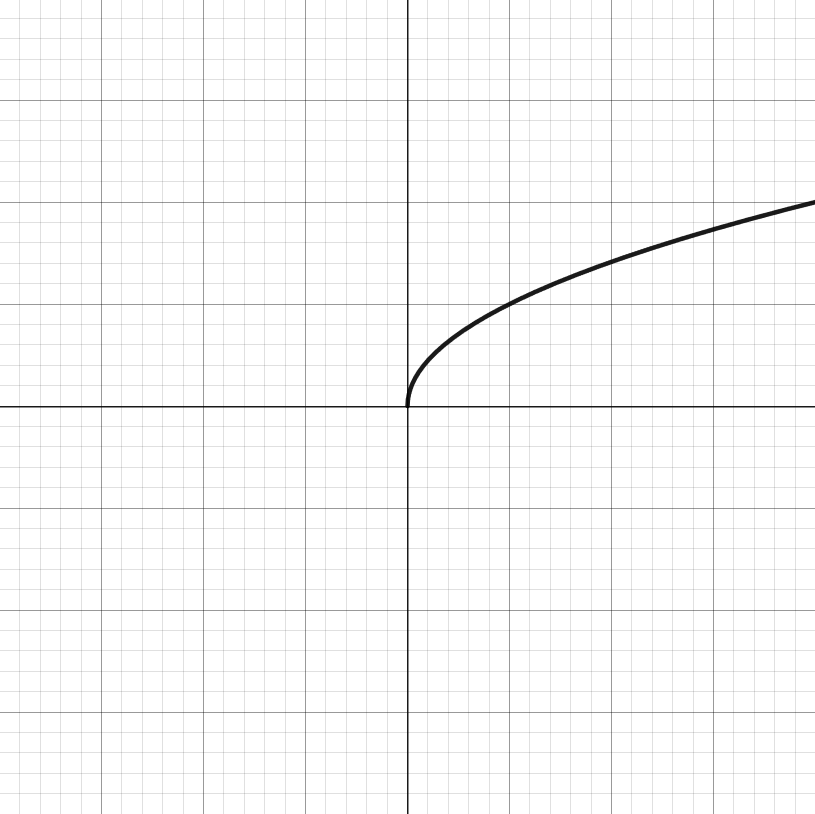
\includegraphics[scale=0.318]{pierwiastkowa.png}} & \fbox{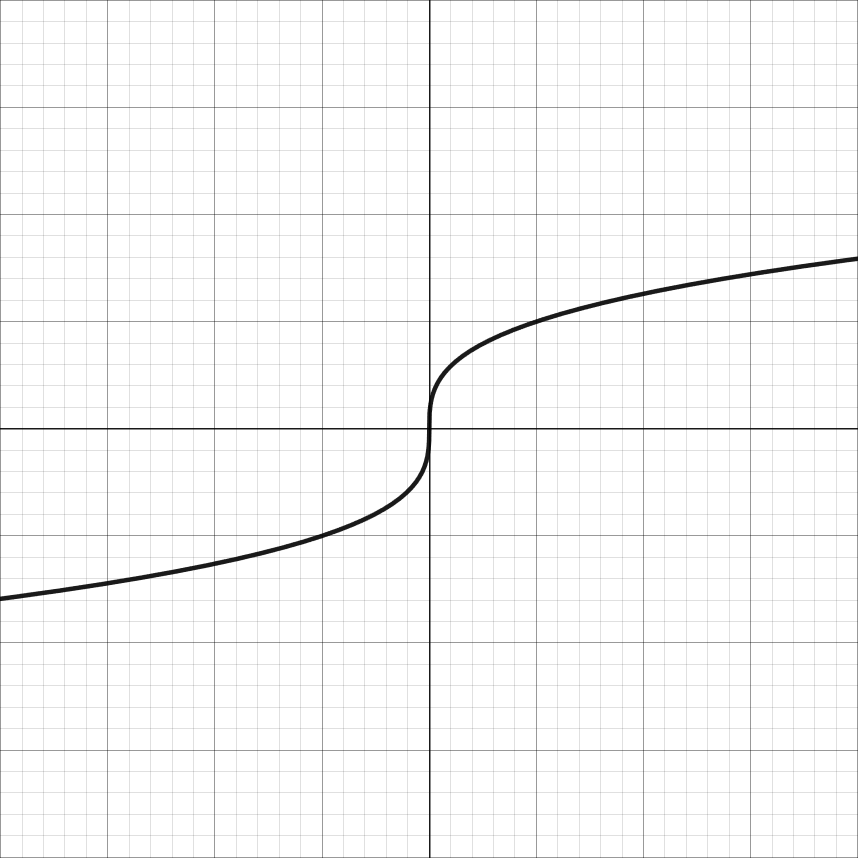
\includegraphics[scale=0.302]{pierwiastkowa trzeciego stopnia.png}}\\
   $f(x) = \sqrt{x} $ & $f(x) = \sqrt[3]{x}$
\end{tabular}

\begin{tabular}{cc}
   \fbox{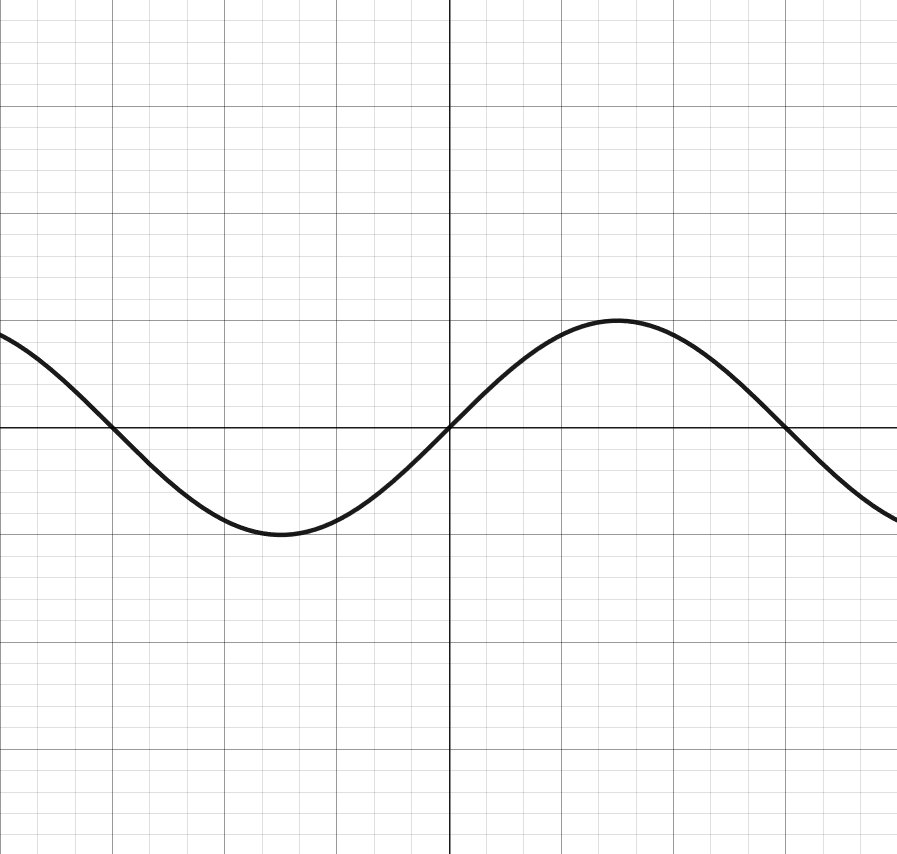
\includegraphics[scale=0.29]{sinus.png}} & \fbox{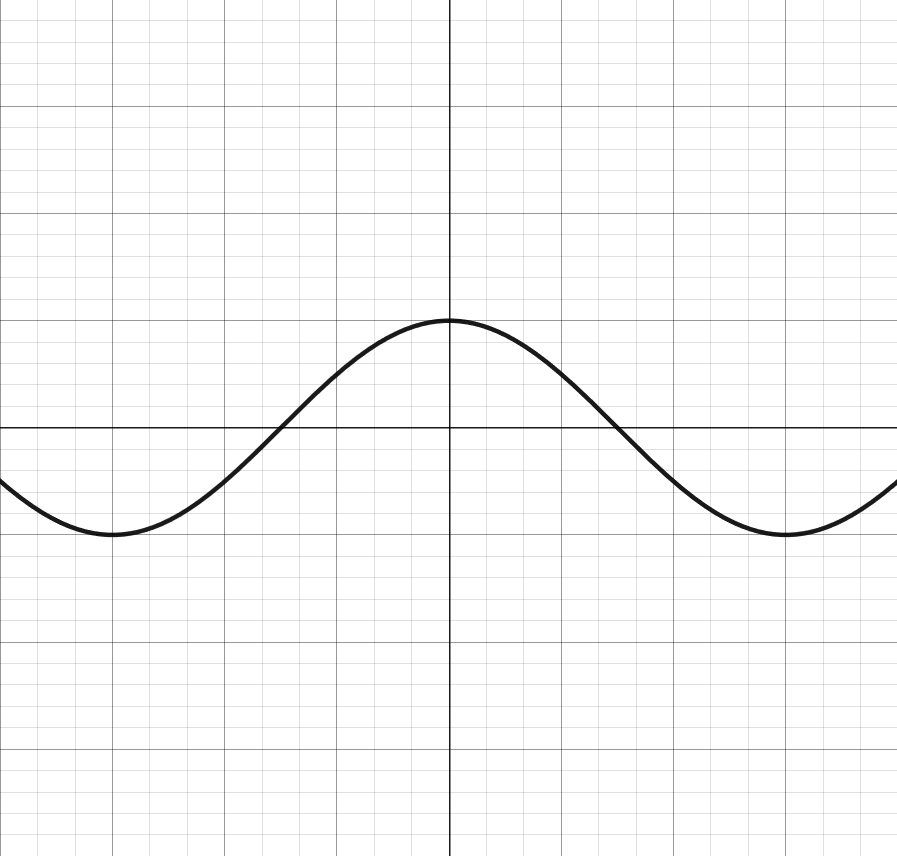
\includegraphics[scale=0.29]{cosinus.png}}\\
   $f(x) = \sin{x}\text{ - }\textbf{sinusoida}$ & $f(x) = \cos{x}\text{ - }\textbf{cosinusoida}$
\end{tabular}

\begin{tabular}{cc}
   \fbox{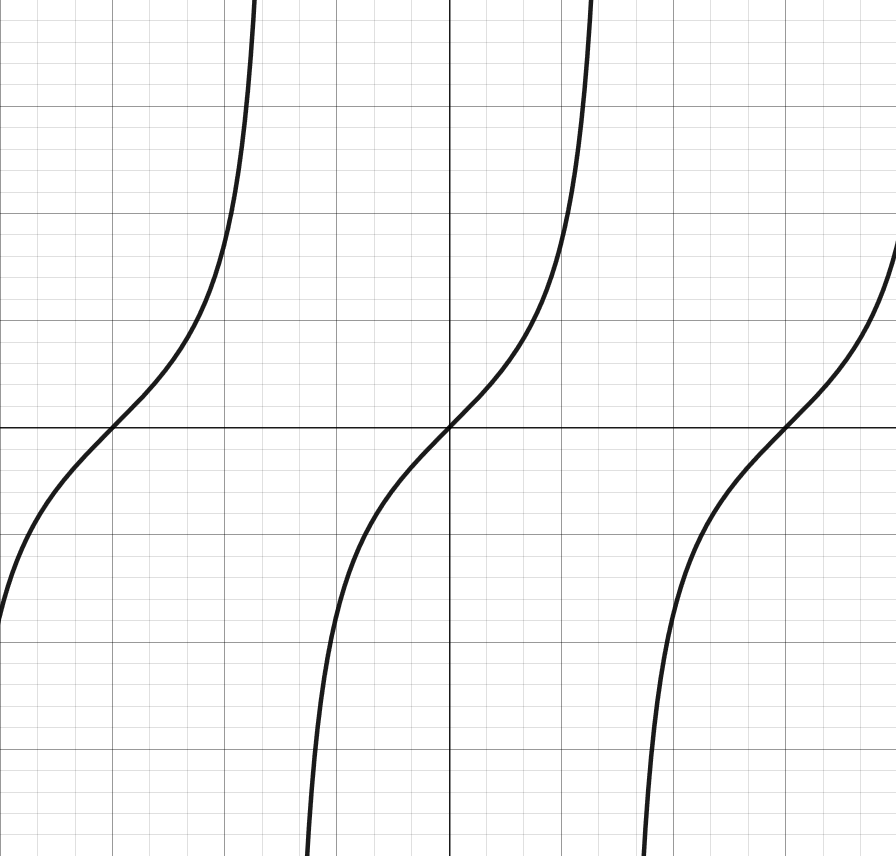
\includegraphics[scale=0.29]{tangens.png}} & \fbox{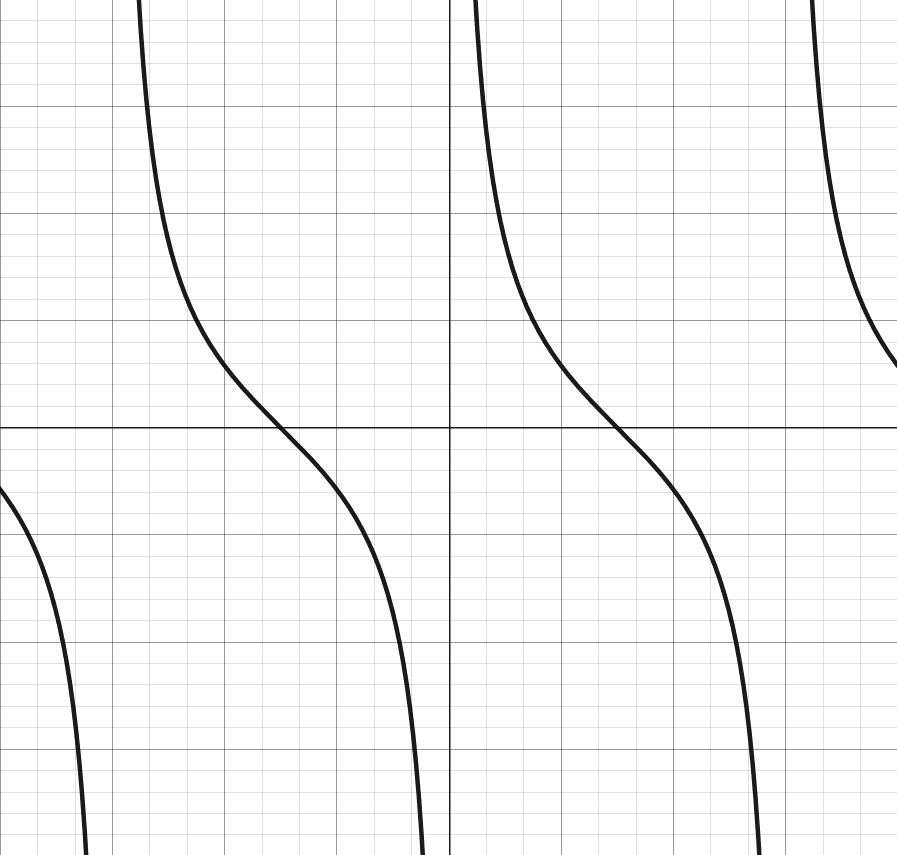
\includegraphics[scale=0.29]{cotangens.png}}\\
   $f(x) = \text{tg}\;x\text{ - }\textbf{tangensoida}$ & $f(x) = \text{ctg}\;x\text{ - }\textbf{cotangensoida}$
\end{tabular}

\begin{tabular}{cc}
   \fbox{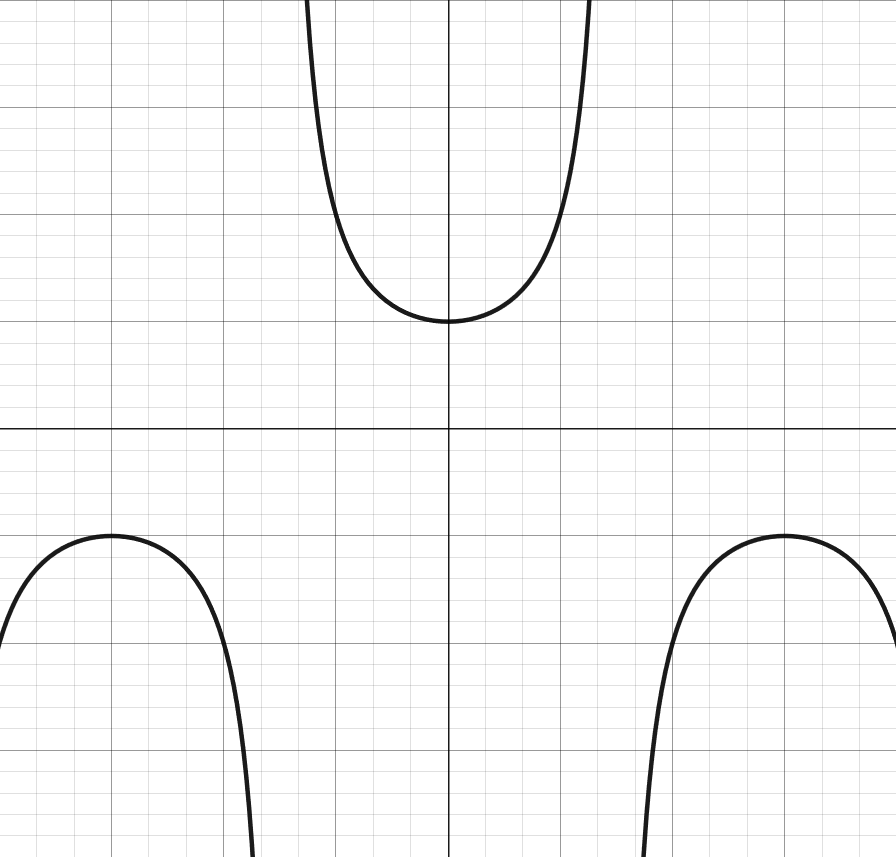
\includegraphics[scale=0.29]{sekans.png}} & \fbox{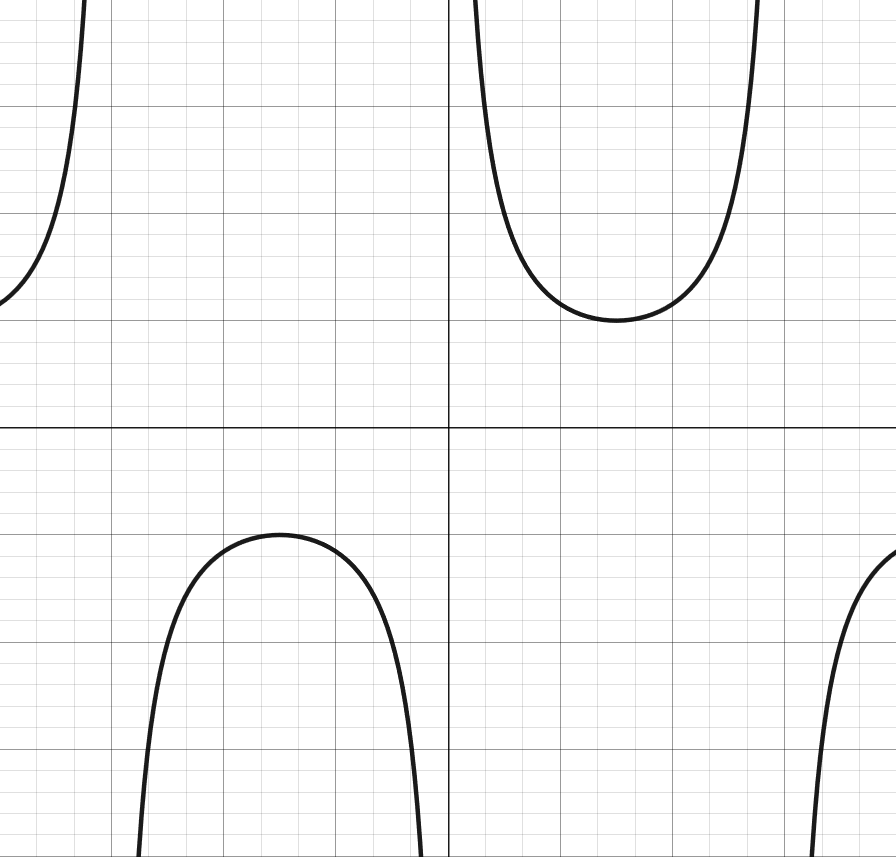
\includegraphics[scale=0.29]{kosekans.png}}\\
   $f(x) = \sec x$ & $f(x) = \text{cosec}\;x$
\end{tabular}

\begin{tabular}{cc}
   \fbox{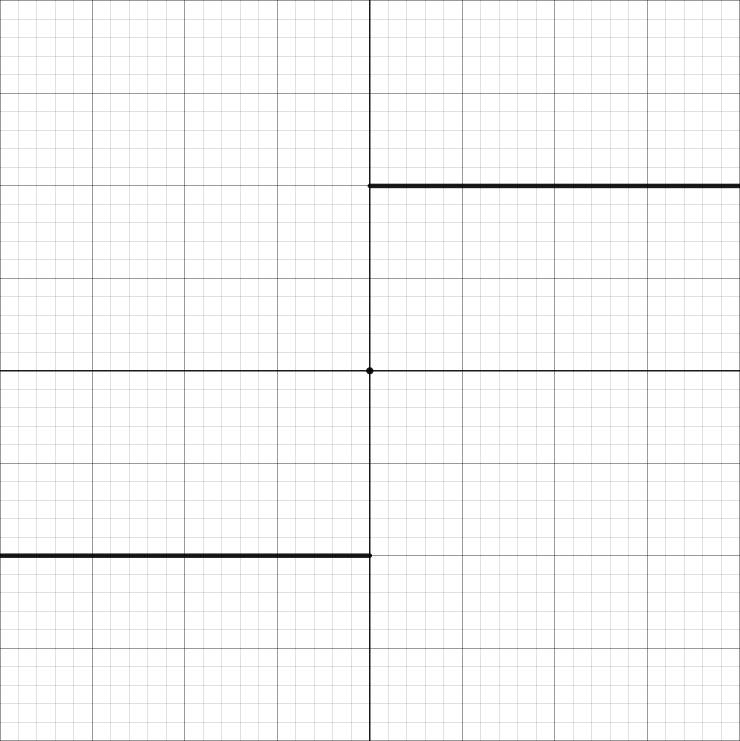
\includegraphics[scale=0.35]{signum.png}} & \fbox{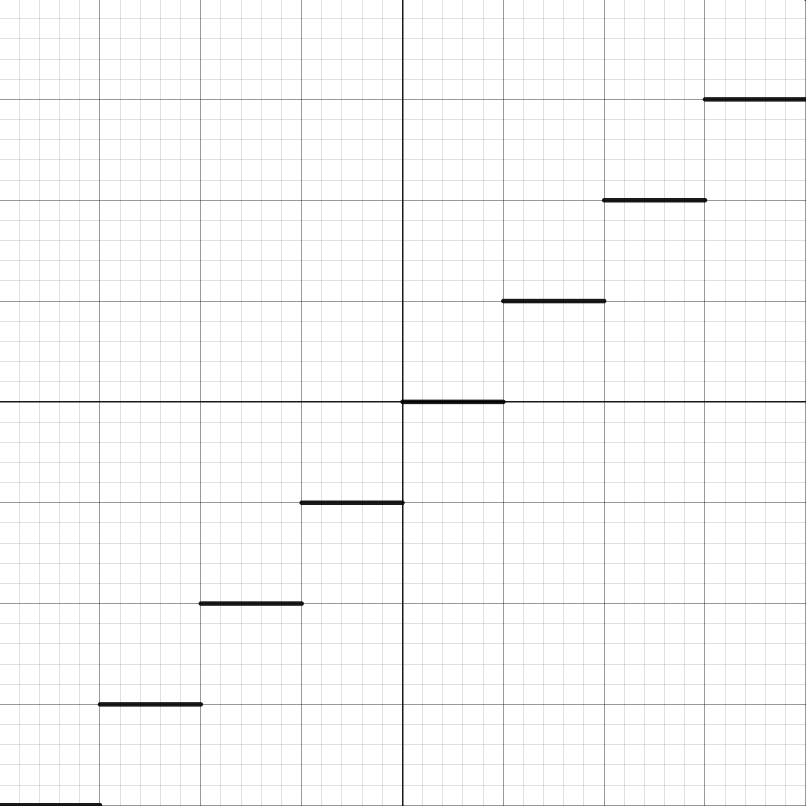
\includegraphics[scale=0.323]{podłoga.png}}\\
   $f(x) = \text{sgn}(x)$ & $f(x) = \lfloor x\rfloor$
\end{tabular}

\end{center}
}%

\subsection{Przekształcenia funkcji}

{%
\setlength{\fboxsep}{0pt}%
\setlength{\fboxrule}{0.5pt}%

\begin{center}
   \begin{tabular}{ll}

     \begin{tabular}{l}
      \vtop{\hbox{\strut Symetria osiowa względem osi OX:} \hbox{\strut $y = -f(x)$}}\\[6cm]
      \vtop{\hbox{\strut Symetria osiowa względem osi OY:} \hbox{\strut $y = f(-x)$}}\\[6cm]
      \vtop{\hbox{\strut Symetria osiowa względem} \hbox{\strut środka układu współrzędnych:} \hbox{\strut $y = -f(-x)$}}\\
     \end{tabular} &


     \begin{tabular}{l}
      \fbox{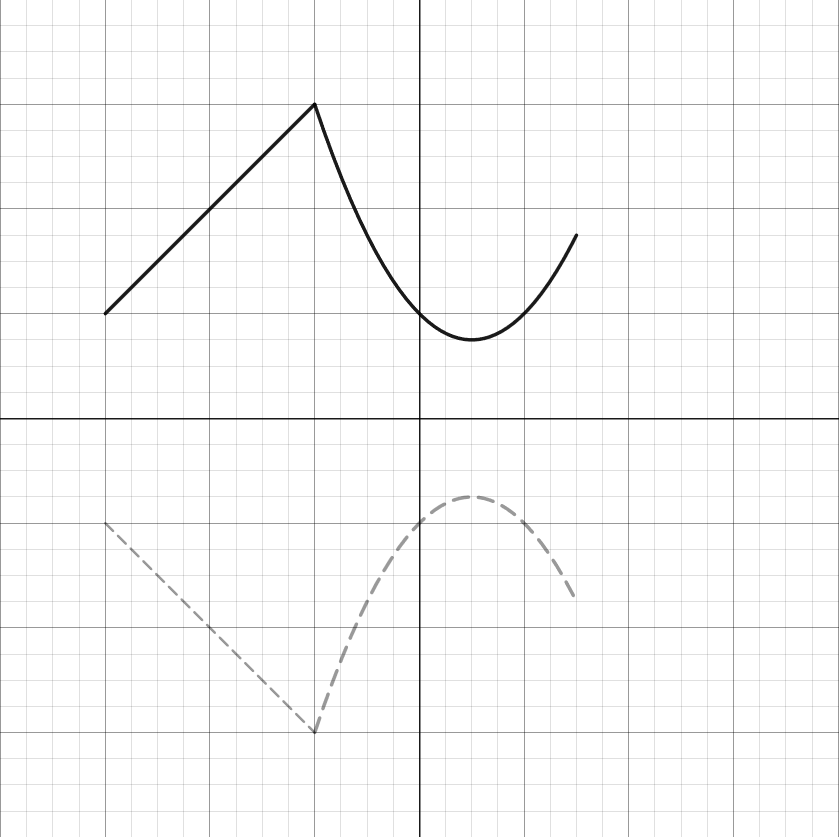
\includegraphics[scale=0.3]{symetria OX.png}}\\
      \fbox{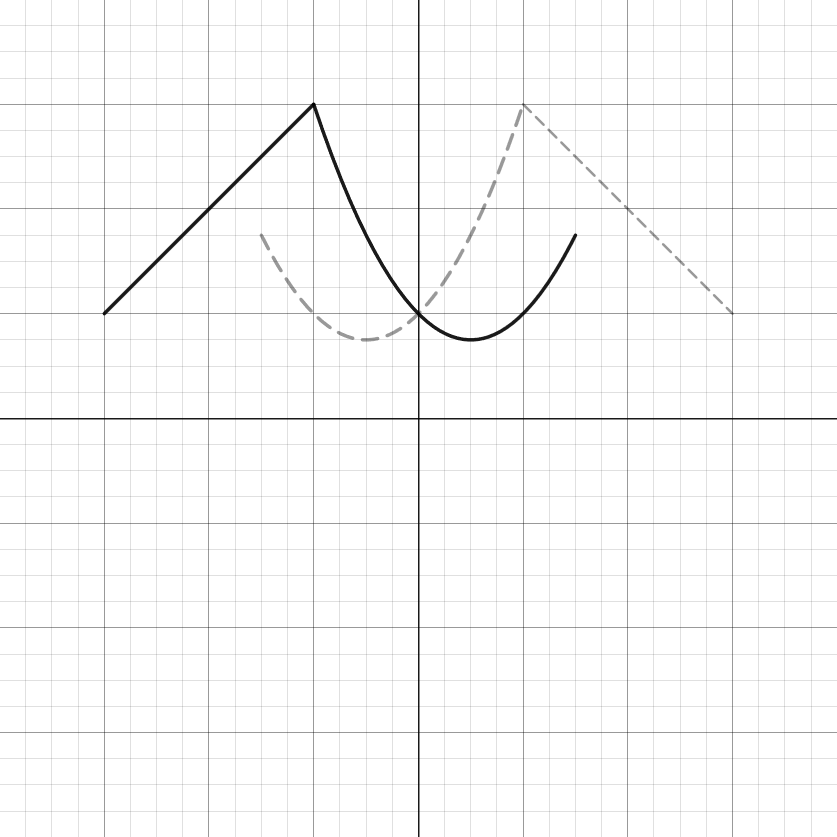
\includegraphics[scale=0.3]{symetria OY.png}}\\
      \fbox{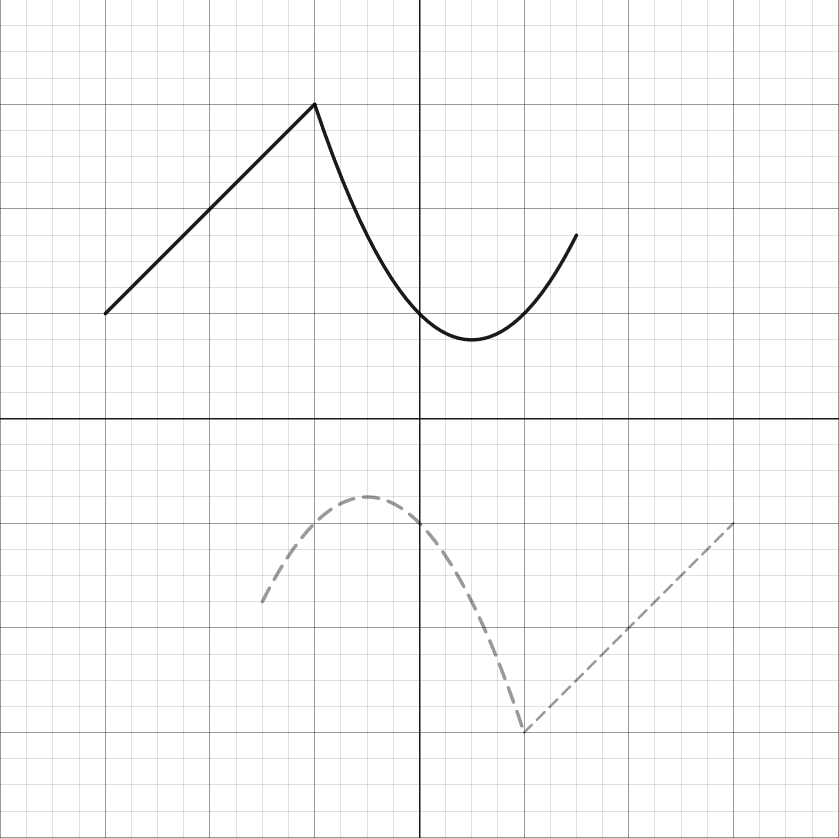
\includegraphics[scale=0.3]{symetria względem środka.png}}\\
     \end{tabular}

   \end{tabular}
   
\end{center}


\begin{center}

   \begin{tabular}{ll}

     \begin{tabular}{l}
      \vtop{\hbox{\strut Przesunięcie równoległe poziome:} \hbox{\strut $y = f(x - a),\;\; \vec{v} = [a,0]$}}\\[6cm]
      \vtop{\hbox{\strut Przesunięcie równoległe pionowe:} \hbox{\strut $y = f(x) + b,\;\; \vec{v} = [0,b]$}}\\[6cm]
      \vtop{\hbox{\strut Przesunięcie równoległe ukośne:} \hbox{\strut $y = f(x - a) + b,\;\; \vec{v} = [a,b]$}}\\
     \end{tabular} &


     \begin{tabular}{l}
      \fbox{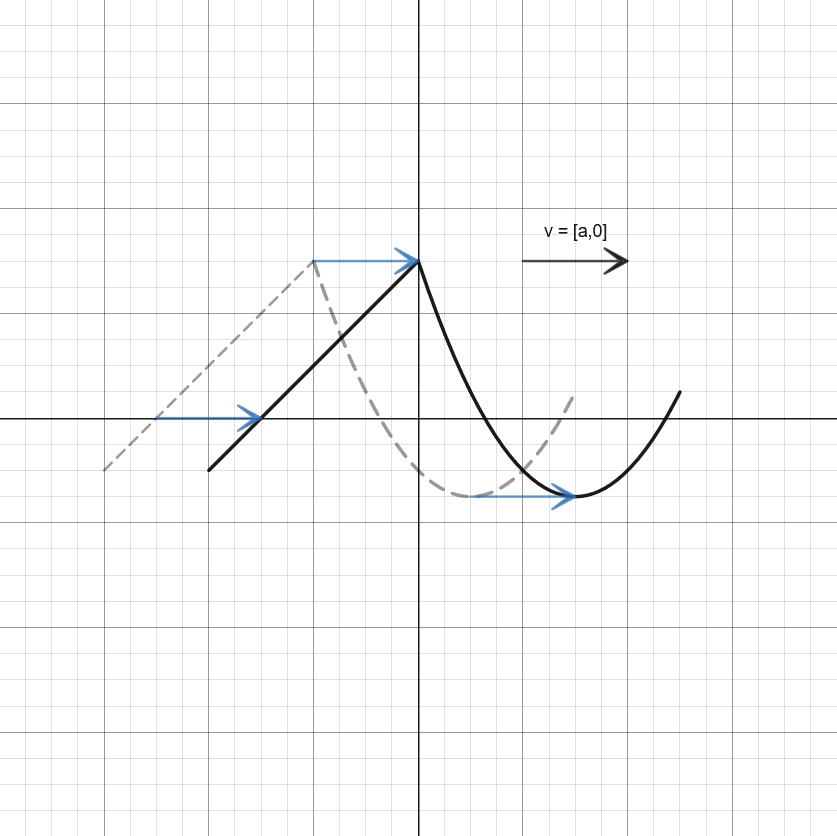
\includegraphics[scale=0.3]{przesunięcie wykresu w bok.png}}\\
      \fbox{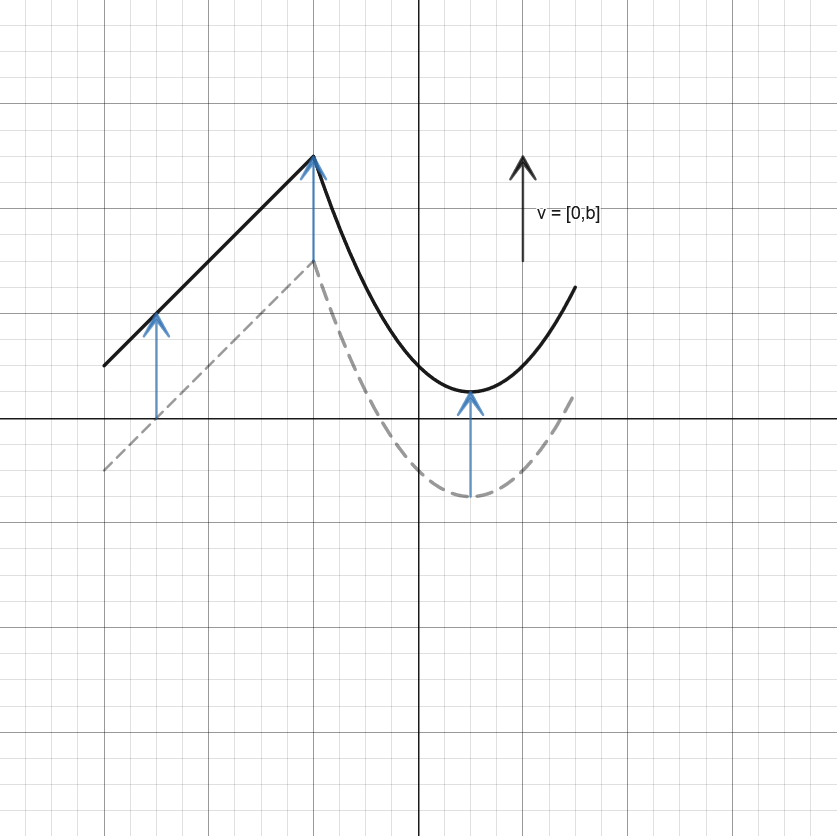
\includegraphics[scale=0.3]{przesunięcie wykresu w górę.png}}\\
      \fbox{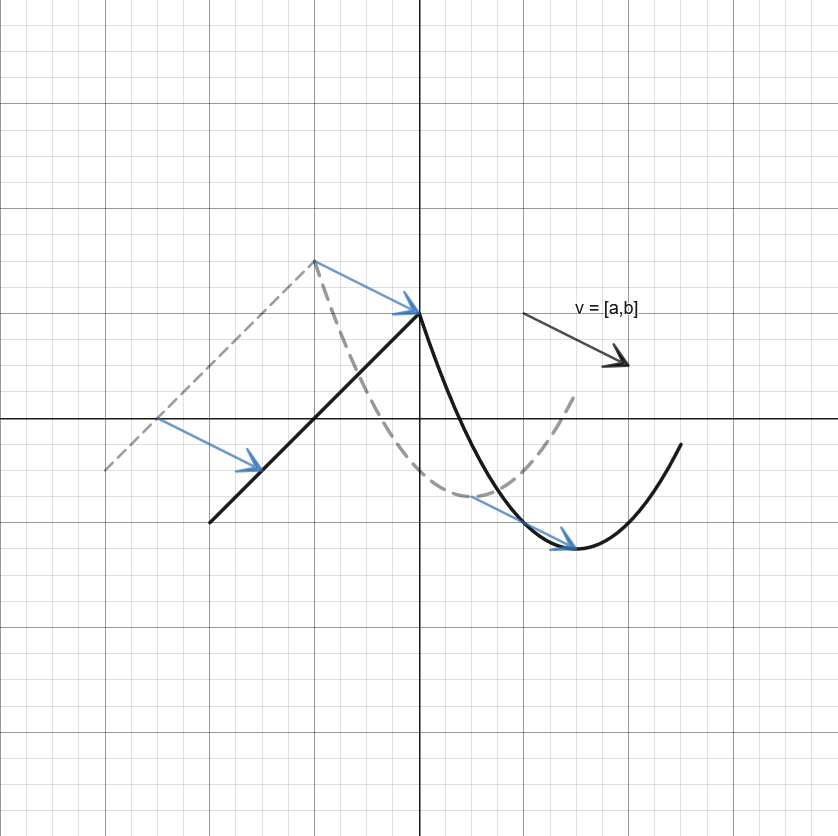
\includegraphics[scale=0.3]{przesunięcie w cholerę.png}}\\
     \end{tabular}

   \end{tabular}
   
\end{center}
}%

{%
\setlength{\fboxsep}{0pt}%
\setlength{\fboxrule}{0.5pt}%

\begin{center}
   \begin{samepage}

   \begin{tabular}{cc}
      \fbox{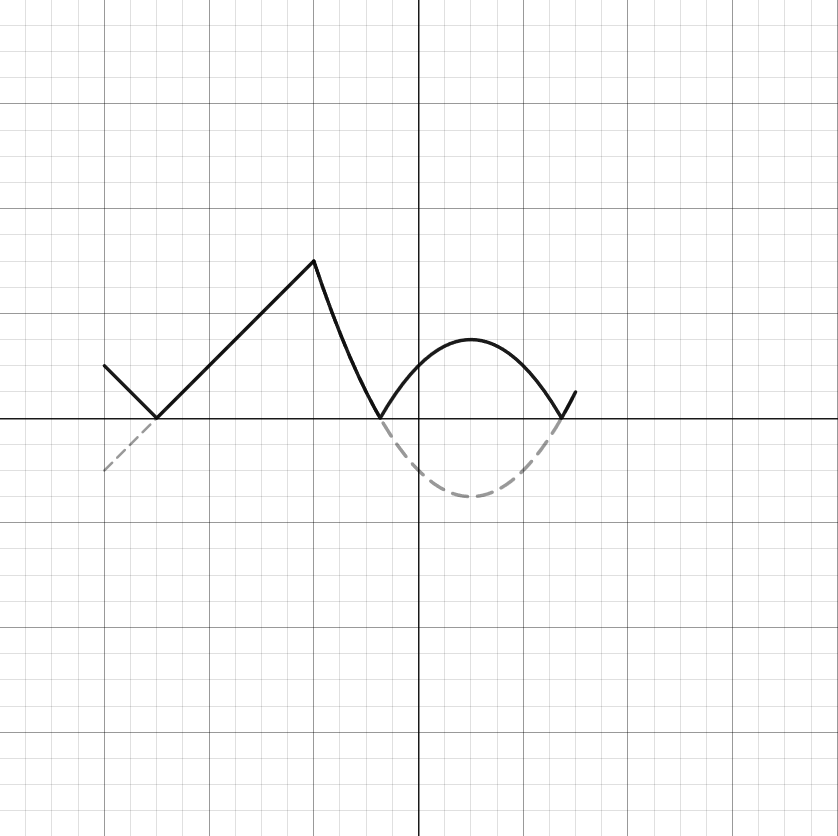
\includegraphics[scale=0.3]{bezwzględna OX.png}} & \fbox{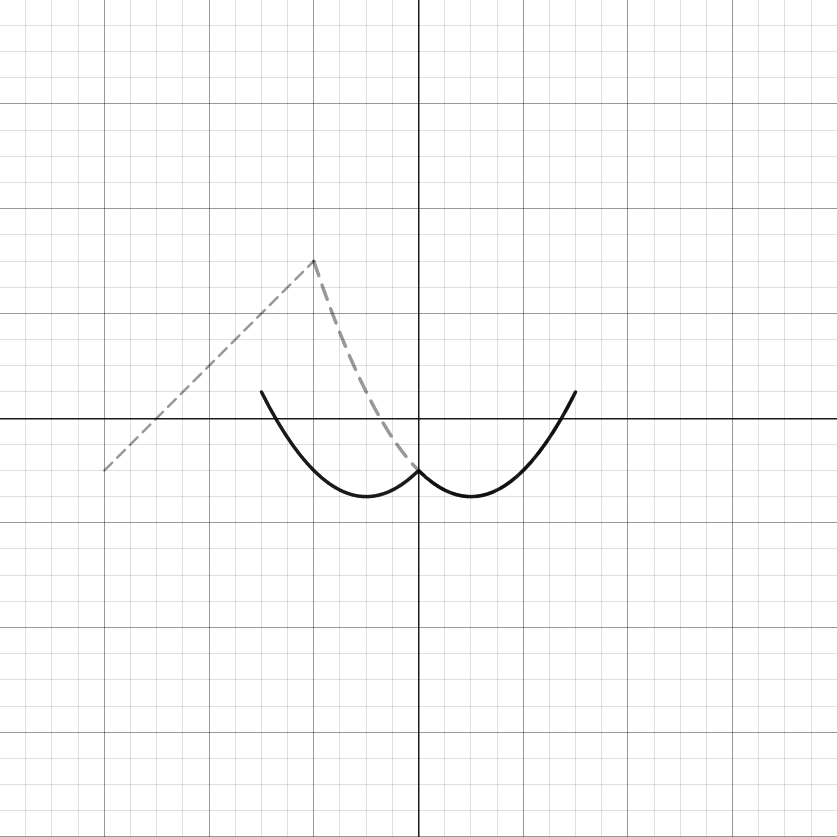
\includegraphics[scale=0.3]{bezwzględna OY.png}}\\
      $y = \vert f(x)\vert$ & $y = f(\vert x\vert)$
   \end{tabular}   
   \nopagebreak[4]
   \begin{tabular}{cc}
      \fbox{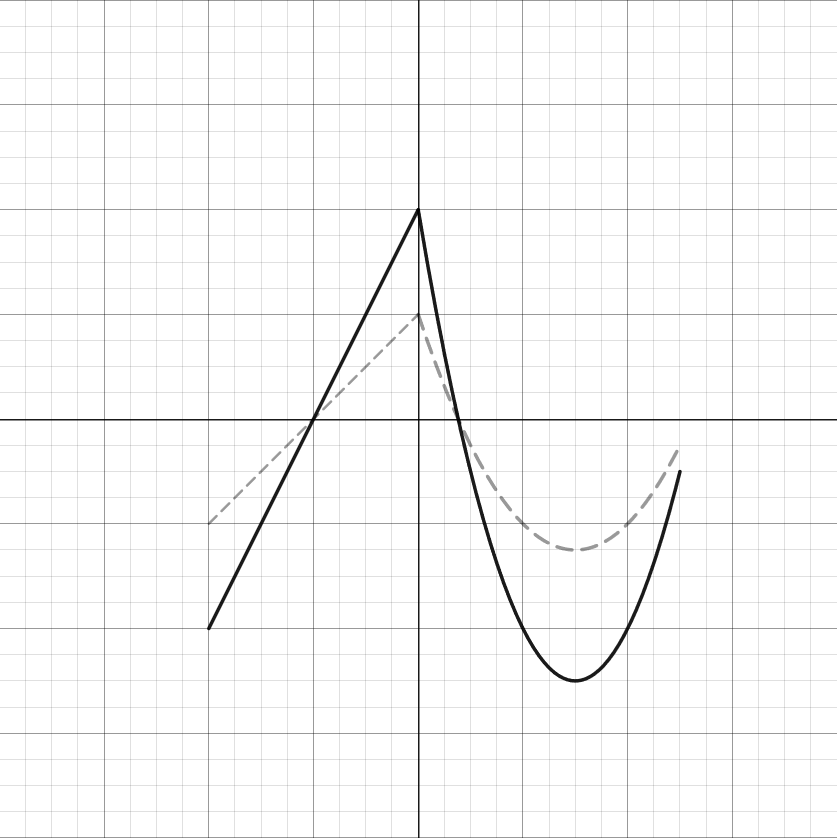
\includegraphics[scale=0.3]{powinowactwo prostokątne OX1.png}} & \fbox{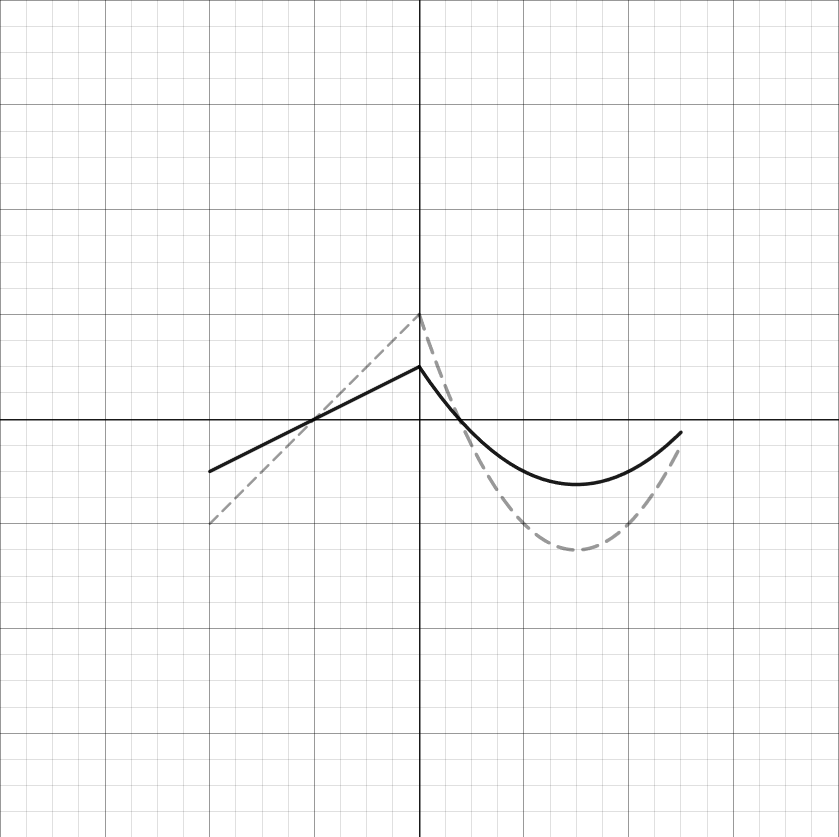
\includegraphics[scale=0.3]{powinowactwo prostokątne OX2.png}}\\
      Powinowactwo prostokątne o & Powinowactwo prostokątne o\\
      osi OX: $y = af(x),\;\;a > 1$ & osi OX: $y = af(x),\;\;0 < a < 1$
   \end{tabular}
   \nopagebreak[4]
   \begin{tabular}{cc}
      \fbox{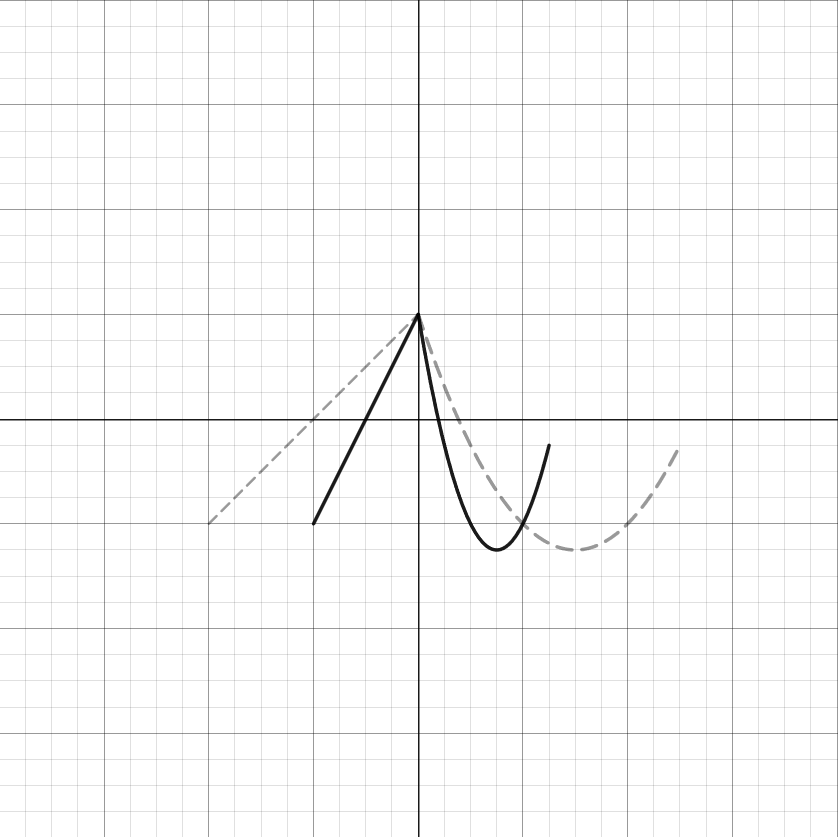
\includegraphics[scale=0.3]{powinowactwo prostokątne OY1.png}} & \fbox{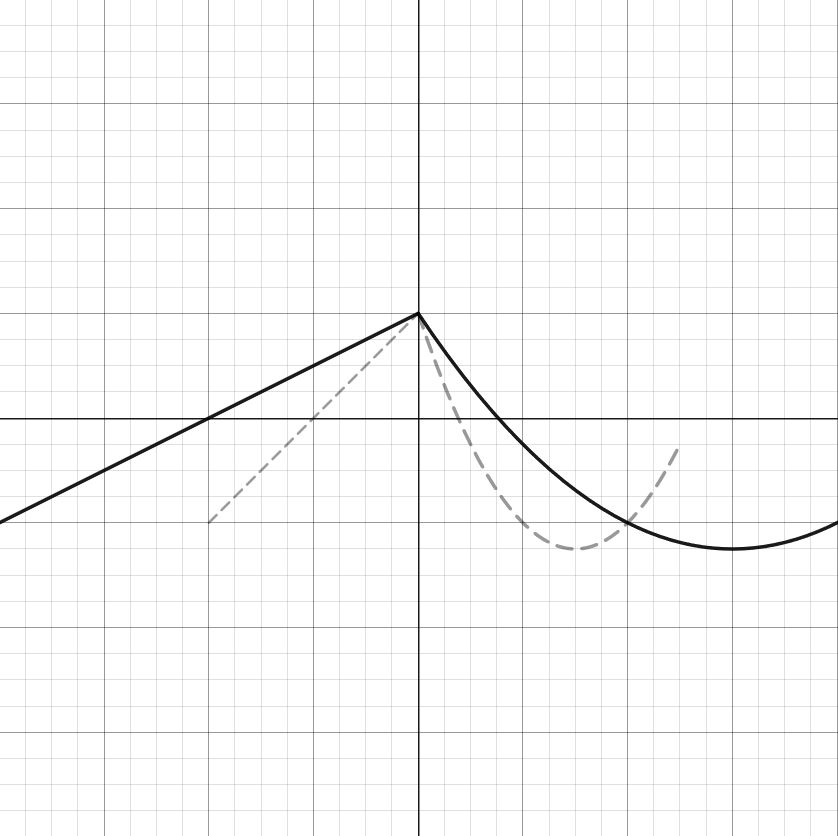
\includegraphics[scale=0.3]{powinowactwo prostokątne OY2.png}}\\
      Powinowactwo prostokątne o & Powinowactwo prostokątne o\\
      osi OY: $y = f(ax),\;\;a > 1$ & osi OY: $y = f(ax),\;\;0 < a < 1$
   \end{tabular}

   \end{samepage}
\end{center}
}%

\newpage

\section{Ciągi}
\subsection{Informacje i twierdzenia}
\noindent\textbf{Ciąg} - Przyporządkowanie zbiorowi liczb $A = \langle 1, n \rangle,\; A \subset \mathbb{N}_{+}$ zwanemu zbiorowi indeksów kolejnych elementów,
zwanymi \textbf{wyrazami ciągu}.\hfill\break\\
\noindent\textbf{Ciąg skończony} to ciąg, w którym występuje skończenie wiele elementów, tj. zbiór
indeksów jest podzbiorem właściwym liczb naturalnych dodatnich.\\
\noindent\textbf{Ciąg nieskończony} to ciąg, w którym występuje nieskończenie wiele elementów, tj. zbiór
indeksów jest zbiorem liczb naturalnych dodatnich.\hfill\break\\

\noindent\textbf{Monotoniczność ciągu}
\begin{itemize}
   \item Stały - wyrazy ciągu są sobie równe dla dowolnej pary indeksów:\\ $\forall n\in\mathbb{N}_{+}\;\; a_{n} = a_{n+1}$
   \item Rosnący - każdy kolejny wyraz jest większy od wyrazu o mniejszym indeksie: $\forall n\in\mathbb{N}_{+}\;\; a_{n} < a_{n+1}$
   \item Niemalejący - każdy kolejny wyraz jest większy od wyrazu bądź równy wyrazowi o mniejszym indeksie: $\forall n\in\mathbb{N}_{+}\;\; a_{n} \leq a_{n+1}$
   \item Nierosnący - każdy kolejny wyraz jest mniejszy od wyrazu bądź równy wyrazowi o mniejszym indeksie: $\forall n\in\mathbb{N}_{+}\;\; a_{n} \geq a_{n+1}$
   \item Malejący - każdy kolejny wyraz jest mniejszy od wyrazu o mniejszym indeksie: $\forall n\in\mathbb{N}_{+}\;\; a_{n} > a_{n+1}$
\end{itemize}
Monotoniczność ciągu można określić, badając znak różnicy kolejnych wyrazów ciągu: $a_{n+1} - a_{n}$.\\
{%

\renewcommand{\arraycolsep}{0.35cm}
\renewcommand{\arraystretch}{1.4}

\begin{center}
\begin{tabular}{ll}
   $a_{n+1} - a_{n} > 0$ & - \; rosnący\\
   $a_{n+1} - a_{n} \geq 0$ & - \; niemalejący\\
   $a_{n+1} - a_{n} \leq 0$ & - \; nierosnący\\
   $a_{n+1} - a_{n} < 0$ & - \; malejący
\end{tabular}
\end{center}
}%

\subsection{Granica ciągu liczbowego}
Liczba $l$ jest granicą nieskończonego ciągu liczbowego $(a_{n})$ wtedy i tylko wtedy, gdy dla
każdej liczby dodatniej $\varepsilon$ istnieje taka liczba $\delta$, że dla każdej liczby naturalnej
$n > \delta$ zachodzi nierówność $\vert a_{n} - l\vert < \varepsilon$, tj. odległość od granicy $l$ do
wartości $a_{n}$ jest mniejsza od $\varepsilon$. Definicja ta jest znana jako definicja epsilon - delta granicy ciągu.\\
$$\lim_{n\to \infty}a_{n} = l \Leftrightarrow \underset{\varepsilon > 0}{\bigwedge} \underset{\delta}{\bigvee} \underset{n > \delta}{\bigwedge} \vert a_{n} - l\vert < \varepsilon$$

\noindent\includegraphics[scale=0.38]{defninicja limit ciągu.png}\\\\
\noindent\textbf{Ciąg zbieżny} to ciąg nieskończony, którego granicą jest liczba rzeczywista.
Taki ciąg ma tylko jedną granicę.\\
Ciąg jest rozbieżny, gdy granicą jest dodatnia bądź ujemna nieskończoność.\\\\

\noindent\textbf{Twierdzenia o działaniach na granicach ciągów zbieżnych}\\
Jeżeli $\underset{n \to \infty}{\lim}a_{n} = a$ i $\underset{n \to \infty}{\lim}b_{n} = b$, to zachodzą następujące równości:
{%

\renewcommand{\arraycolsep}{1cm}
\renewcommand{\arraystretch}{1.8}

\begin{equation*}
\begin{array}{cc}
   \underset{n \to \infty}{\lim}(a_{n} + b_{n}) = a + b & \underset{n \to \infty}{\lim}(a_{n} - b_{n}) = a - b\\
   \underset{n \to \infty}{\lim}(a_{n}\cdot b_{n}) = a\cdot b & \underset{n \to \infty}{\lim}\left(\dfrac{a_{n}}{b_{n}}\right) = \dfrac{a}{b}
\end{array}
\end{equation*}
}%

\newpage

\subsection{Ciąg arytmetyczny}
\noindent Niech ciąg $(a_{n})$ będzie przynajmniej trzywyrazowy. Wtedy ciągiem arytmetycznym nazywamy takie $(a_{n})$,
gdzie każdy kolejny wyraz oprócz pierwszego jest tworzony poprzez dodanie stałej $r$, nazywanej \textbf{różnicą ciągu arytmetycznego}.\\\\
\noindent\textbf{Postać rekurencyjna}
$$a_{n+1} = a_{n} + r$$
\noindent\textbf{Postać jawna}
$$a_{n} = a_{1} + (n - 1)r$$
\noindent\textbf{Wzór na różnicę ciągu}
$$r = a_{n} - a_{n+1}$$
\noindent\textbf{Wzór na sumę $n$ początkowych wyrazów ciągu}
$$S_{n} = \dfrac{a_{1} + a_{n}}{2}\cdot n = \dfrac{2a_{1} + (n - 1)r}{2}\cdot n$$
\noindent\textbf{Warunek wystarczający ciągu arytmetycznego}
$$a_{n} = \dfrac{a_{n-1}+a_{n+1}}{2}$$


\subsection{Ciąg geometryczny}
\noindent Niech ciąg $(a_{n})$ będzie przynajmniej trzywyrazowy. Wtedy ciągiem geometrycznym nazywamy takie $(a_{n})$,
gdzie każdy kolejny wyraz oprócz pierwszego jest tworzony poprzez pomnożenie przez stałą $q$, nazywaną \textbf{ilorazem ciągu arytmetycznego}.\\\\
\noindent\textbf{Postać rekurencyjna}
$$a_{n+1} = a_{n}\cdot q$$
\noindent\textbf{Postać jawna}
$$a_{n} = a_{1} \cdot q^{n-1}$$
\noindent\textbf{Wzór na iloraz ciągu}
$$q = \dfrac{a_{n+1}}{a_{n}}$$
\noindent\textbf{Wzór na sumę $n$ początkowych wyrazów ciągu}
$$S_{n} = a_{1}\cdot\dfrac{1-q^{n}}{1-q},\; q \neq 1\;\;\;\;\; a_{1}\cdot n,\; q = 1$$
\noindent\textbf{Warunek wystarczający ciągu geometrycznego}
$$a_{n} = \sqrt{a_{n-1}\cdot a_{n+1}}$$
\\

\noindent Dla $\vert q\vert < 1$ ciąg geometryczny staje się zbieżny i można go rozważać jako \textbf{szereg geometryczny}.
Sumę wszystkich wyrazów szeregu geometrycznego można wyliczyć ze wzoru:
$$S = \dfrac{a_{1}}{1-q}$$

\newpage






\section{Elementy analizy matematycznej}
\subsection{Granica funkcji}
\noindent\textbf{Granica} - wartość, do której wartości funkcji zbliżają się nieograniczenie dla argumentów
z dziedziny funkcji arbitralnie bliskich punktowi. Operację tą notuje się symbolem $\displaystyle\lim_{x\to n}$ nazywanym \textit{limesem}, czytanym ''Limes przy $x$ dążącym do $n$''.\hfill\break\\

\noindent\textbf{Definicja Cauchy'ego granicy funkcji} - Liczba $l$ jest granicą funkcji $f$ w punkcie $x_{0}$ wtedy i tylko wtedy, gdy dla
każdej liczby dodatniej $\varepsilon$ istnieje taka liczba $\delta > 0$, że dla każdego elementu dziedziny funkcji $f(x), \; f: X \rightarrow \mathbb{R}$, takiego że
$x \in X \cap (x_{0} - \delta,\; x_{0} + \delta)$ prawdziwa jest zależność: $\vert f(x) - l\vert < \varepsilon$.\\
$$\lim_{x\to x_{0}} f(x) = l \Leftrightarrow $$
$$\underset{\varepsilon > 0}{\bigwedge} \;\underset{\delta > 0}{\bigvee} \; \underset{x \in A}{\bigwedge} \; \vert f(x) - l\vert < \varepsilon, \;\; A = \{x:x\in X \land 0 < \vert x - x_{0}\vert < \delta\}$$
\begin{center}
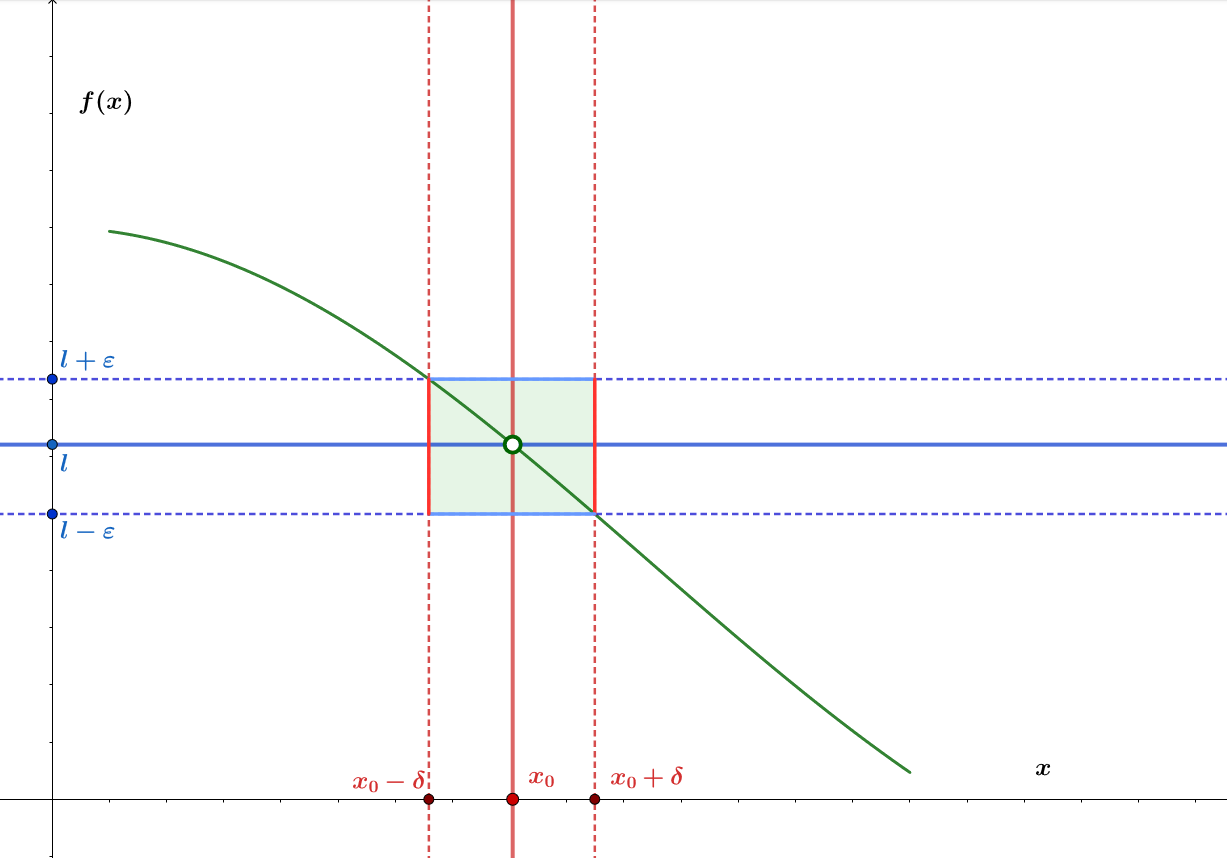
\includegraphics[scale=0.51]{limit funkcji.png}
\end{center}

\newpage
\noindent\textbf{Definicja Heinego} - Funkcja $f$ ma granicę $l$ w punkcie $x_{0}$ wtedy i tylko wtedy,
gdy dla każdego ciągu $(x_{n}), n \in \mathbb{N}$ zbieżnego do $x_{0}$, zdefiniowanego na podzbiorze dziedziny $X$ który
to podzbiór ma w punkcie skupienia $x_{0}$ (podzbiór ten nazywa się sąsiedztwem $S(x_{0})$), wartość funkcji od ciągu $(x_{n})$, czyli $f(x_{n})$ jest zbieżna do $l$.

\subsection{Granica jednostronna}
\noindent Granica jednostronna to wspólna nazwa na granicę \textit{lewostronną} i \textit{prawostronną}.\\\\
\noindent\textbf{Granica lewostronna} - wartość w punkcie $x_{0}$, do której wartości funkcji zbliżają się nieograniczenie,
ale uwzględniając tylko argumenty z dziedziny mniejsze od rozważanego punktu. By ten fakt odzwierciedlić, definicje
granicy są zmodyfikowane w następujący sposób:\\

\noindent\textbf{Definicja Cauchy'ego}
$$\lim_{x\to x_{0}^{-}} f(x) = l \Leftrightarrow $$
$$\underset{\varepsilon > 0}{\bigwedge} \;\underset{\delta > 0}{\bigvee} \; \underset{x \in A}{\bigwedge} \; \vert f(x) - l\vert < \varepsilon, \;\; A = \{x:x\in X \land x - \delta < x < x_{0}\}$$
\noindent\textbf{Definicja Heinego}\\
Rozpatrywane jest tylko sąsiedztwo $S(x_{0})$, gdzie $\forall x \in S(x_{0})\; x < x_{0}$.\\\\

\noindent\textbf{Granica prawostronna} - wartość w punkcie $x_{0}$, do której wartości funkcji zbliżają się nieograniczenie,
ale uwzględniając tylko argumenty z dziedziny większe od rozważanego punktu. By ten fakt odzwierciedlić, definicje
granicy są zmodyfikowane w następujący sposób:\\

\noindent\textbf{Definicja Cauchy'ego}
$$\lim_{x\to x_{0}^{+}} f(x) = l \Leftrightarrow $$
$$\underset{\varepsilon > 0}{\bigwedge} \;\underset{\delta > 0}{\bigvee} \; \underset{x \in A}{\bigwedge} \; \vert f(x) - l\vert < \varepsilon, \;\; A = \{x:x\in X \land x_{0} < x < x + \delta\}$$
\noindent\textbf{Definicja Heinego}\\
Rozpatrywane jest tylko sąsiedztwo $S(x_{0})$, gdzie $\forall x \in S(x_{0})\; x > x_{0}$.\\\\

\noindent Jeżeli granica lewostronna oraz prawostronna w punkcie $x_{0}$ są sobie równe, jest to warunek wystarczający
dla istnienia granicy w tym punkcie:
$$\lim_{x\to x_{0}}f(x) = l \; \Leftrightarrow \; \lim_{x\to x_{0}^{-}}f(x) = \lim_{x\to x_{0}^{+}}f(x) = l$$
Jeżeli granica lewostronna i prawostronna w punkcie są różne, wtedy granica w tym punkcie nie istnieje.\\

\subsection{Granica niewłaściwa}
Granica niewłaściwa to granica, której wartość w punkcie $x_{0}$ jest równa minus $(-\infty)$ lub plus $(+\infty)$ nieskończoności.
Granica w punkcie jest niewłaściwa, gdy spełnione są następujące warunki równoważnych definicji:\\

\noindent\textbf{Definicja Cauchy'ego}
$$\lim_{x\to x_{0}} f(x) = +\infty \Leftrightarrow $$
$$\underset{M > 0}{\bigwedge} \;\underset{\delta > 0}{\bigvee} \; \underset{x \in A}{\bigwedge} \; f(x) > M, \;\; A = \{x:x\in X \land 0 < \vert x - x_{0}\vert < \delta\},$$
$$\lim_{x\to x_{0}} f(x) = -\infty \Leftrightarrow $$
$$\underset{M > 0}{\bigwedge} \;\underset{\delta > 0}{\bigvee} \; \underset{x \in A}{\bigwedge} \; f(x) < -M, \;\; A = \{x:x\in X \land 0 < \vert x - x_{0}\vert < \delta\}$$
\noindent\textbf{Definicja Heinego}\\
Funkcja $f$ ma granicę $\pm\infty$ w punkcie $x_{0}$ wtedy i tylko wtedy,
gdy dla każdego ciągu $(x_{n}), n \in \mathbb{N}$ zbieżnego do $x_{0}$, zdefiniowanego na podzbiorze dziedziny $X$ który
to podzbiór ma w punkcie skupienia $x_{0}$, wartość funkcji od ciągu $(x_{n})$, czyli $f(x_{n})$ jest zbieżna do $\pm\infty$.


\subsection{Granica w nieskończoności}
Granica w nieskończoności przyjmuje wartość $l$ gdy spełnione są następujące warunki równoważnych definicji:\\

\noindent\textbf{Definicja Cauchy'ego}
$$\lim_{x\to +\infty} f(x) = l \Leftrightarrow \underset{\varepsilon > 0}{\bigwedge} \;\underset{\mu \in \mathbb{R}}{\bigvee} \; \underset{x > \mu}{\bigwedge} \; \vert f(x) - l \vert < \varepsilon,$$
\nopagebreak[4]
$$\lim_{x\to -\infty} f(x) = l \Leftrightarrow \underset{\varepsilon > 0}{\bigwedge} \;\underset{\mu \in \mathbb{R}}{\bigvee} \; \underset{x < \mu}{\bigwedge} \; \vert f(x) - l \vert < \varepsilon,$$

\noindent\textbf{Definicja Heinego}\\
Funkcja $f$ ma granicę $l$ w $\pm\infty$ wtedy i tylko wtedy,
gdy dla każdego ciągu $(x_{n}), n \in \mathbb{N}$ zbieżnego do $\pm\infty$, zdefiniowanego na podzbiorze dziedziny $X$, 
odpowiednio $(a, +\infty)$ i $(-\infty, a)$, wartość funkcji od ciągu $(x_{n})$, czyli $f(x_{n})$ dąży do $l$.\\\\

\noindent Granica niewłaściwa w nieskończoności występuje tylko wtedy, gdy granica spełnia warunki granicy niewłaściwej i granicy w nieskończoności.\\

\subsection{Własności granic}
\noindent Niech funkcje $f,g :X \subseteq \mathbb{R} \rightarrow Y$ mają granice właściwe. Wtedy:

{%

\renewcommand{\arraystretch}{2}
%$\displaystyle \lim_{x \to x_{0}}f(x) = a$ i $\displaystyle \lim_{x \to x_{0}}g(x) = b \neq 0$

\begin{equation*}
\begin{array}{rccc}
   \displaystyle\lim_{x \to x_{0}} & \displaystyle[f(x) + g(x)] & = & \displaystyle\lim_{x \to x_{0}}f(x) + \lim_{x \to x_{0}}g(x) \\
   \displaystyle\lim_{x \to x_{0}} & \displaystyle[f(x) - g(x)] & = & \displaystyle\lim_{x \to x_{0}}f(x) - \lim_{x \to x_{0}}g(x) \\
   \displaystyle\lim_{x \to x_{0}} & \displaystyle[f(x)\cdot g(x)] & = & \displaystyle\lim_{x \to x_{0}}f(x) \cdot \lim_{x \to x_{0}}g(x) \\
   \displaystyle\lim_{x \to x_{0}} & \displaystyle[c \cdot f(x)] & = & \displaystyle c \cdot \lim_{x \to x_{0}}f(x) \\
   \displaystyle\lim_{x \to x_{0}} & \displaystyle\left[\frac{f(x)}{g(x)}\right] & = & \displaystyle\frac{\displaystyle\lim_{x \to x_{0}}f(x)}{\displaystyle\lim_{x \to x_{0}}g(x)} \\
   \displaystyle\lim_{x \to x_{0}} & \displaystyle [f(x)^{g(x)}]& = & \displaystyle \lim_{x \to x_{0}}f(x)^{\lim\limits_{x \to x_{0}}g(x)}
\end{array}   
\end{equation*}

}%

\subsection{Symbole nieoznaczone}
\noindent Wyrażenia algebraiczne które nie mają sensu liczbowego, często występujące przy poszukiwaniu limitów.
Jest ich siedem:
\begin{equation*}
   \begin{array}{ccccccc}
      \dfrac{0}{0} & \dfrac{\pm\infty}{\pm\infty} & 0 \cdot \pm\infty & \infty - \infty & 0^{0} & \infty^{0} & 1^{\pm\infty}
   \end{array}
\end{equation*}
Takie wyniki nie są końcowymi rozwiązaniami i funkcję należy przekształcić, by otrzymać właściwy wynik.

\noindent\textbf{Reguła de L'Hôpitala} (czyt. delopitala) - Reguła umożliwiająca wyznaczenie granic wyrażeń,
których wynikiem jest symbol nieoznaczony.\\
Jeżeli funkcje $f,g:X \rightarrow Y$ są ciągłe oraz:
\begin{itemize}
   \item \textbf{Granice funkcji są nieoznaczone}: $\displaystyle \lim_{x\to x_{0}}f(x) = \lim_{x\to x_{0}}g(x) = 0 \text{ lub } \pm\infty$,
   \item \textbf{Funkcje $f(x)$ i $g(x)$ są różniczkowalne},
   \item \textbf{Pochodna $g^{\prime}(x)$ jest różna od 0},
   \item \textbf{Istnieje granica ilorazu funkcji $f(x)$ i $g(x)$},
\end{itemize}
Wtedy:
$$\lim_{x \to x_{0}}\dfrac{f(x)}{g(x)} = \lim_{x \to x_{0}}\dfrac{f^{\prime}(x)}{g^{\prime}(x)}$$\hfill\break
\noindent\textit{Przykład:}
$$\lim_{x\to 5}\frac{x^{2}-25}{2x^{2}-9x-5} = \frac{25-25}{2\cdot 25 - 9 \cdot 5 -5} = \frac{0}{0}$$
\\\noindent\textit{Stosując regułę de L'Hôpitala:}
$$\lim_{x\to 5}\frac{x^{2}-25}{2x^{2}-9x-5} = \lim_{x\to 5}\frac{(x^{2}-25)^{\prime}}{(2x^{2}-9x-5)^{\prime}} = \lim_{x\to 5}\frac{2x}{4x-9} = \frac{2\cdot 5}{4\cdot 5 - 9} = \frac{10}{11}$$
Reguła de L'Hôpitala działa również dla granic nieoznaczonych w nieskończoności.

\subsection{Definicja ciągłości funkcji}
Niech funkcja $f$ będzie zdefiniowana w pewnym otoczeniu. Jeżeli istnieje granica właściwa
w punkcie $f(x)$ oraz prawdziwa jest równość: $\lim\limits_{x \to x_{0}}f(x) = f(x_{0})$, to
funkcja w tym punkcie jest ciągła. Funkcja jest ciągła w przedziale, jeżeli każdy punkt w przedziale
spełnia powyższe warunki. By całą funkcję można było nazwać ciągłą, warunki te muszą zachodzić na 
całej dziedzinie funkcji\\
Funkcje: wielomianowe, wymierne, potęgowe, wykładnicze, logarytmiczne i trygonometryczne są ciągłe.

\subsection{Limity a asymptoty wykresu}
\begin{itemize}
   \item Asymptota pionowa jednostronna\\
   Niech funkcja $f$ będzie określona w prawostronnym (lewostronnym) sąsiedztwie punktu $x_{0}$.
   Prosta o równaniu $x = x_{0}$ jest asymptotą pionową prawostronną (lewostronną) wykresu funkcji $f$
   wtedy i tylko wtedy, gdy $\lim\limits_{x \to x^{+}_{0}}f(x) = \pm\infty$ $\left(\lim\limits_{x \to x^{-}_{0}}f(x) = \pm\infty\right)$.\\
   \item Asymptota pionowa obustronna\\
   Jeżeli prosta o równaniu $x = x_{0}$ jest jednocześnie asymptotą pionową lewostronną i prawostronną
   wykresu funkcji $f$, to wtedy nazywa się ją asymptotą pionową obustronną.\\
   \item Asymptota pozioma jednostronna\\
   Niech funkcja $f$ będzie określona w przedziale $(m, +\infty)$ (odpowiednio $(-\infty, m)$), $m \in \mathbb{R}$.
   Prosta o równaniu $y = a$ jest asymptotą poziomą prawostronną (lewostronną) wykresu funkcji $f$ 
   wtedy i tylko wtedy, gdy $\lim\limits_{x\to +\infty}f(x) = a$ $\left(\lim\limits_{x\to -\infty}f(x) = a\right)$.\\
   \item Asymptota pozioma obustronna\\
   Jeżeli prosta o równaniu $y = a$ jest jednocześnie asymptotą poziomą lewostronną i prawostronną
   wykresu funkcji $f$, to wtedy nazywa się ją asymptotą poziomą obustronną.\\
   \item Asymptota ukośna jednostronna\\
   Niech funkcja $f$ będzie określona w przedziale $(m, +\infty)$ (odpowiednio $(-\infty, m)$), $m \in \mathbb{R}$.
   Prosta o równaniu $y = ax + b$ jest asymptotą ukośną prawostronną (lewostronną) wykresu funkcji $f$
   wtedy i tylko wtedy, gdy:
   $$\lim_{x \to \pm\infty}\left[f(x) - (ax + b)\right] = 0; \;\; a = \lim_{x \to \pm\infty}\frac{f(x)}{x}, \;\; b = \lim_{x \to \pm\infty}\left[f(x) - ax\right]$$\
   Jeżeli $a = 0$, prosta $y = b$ jest asymptotą poziomą wykresu funkcji $f$.\\
   \item Asymptota ukośna obustronna\\
   Jeżeli prosta o równaniu $y = ax + b$ jest jednocześnie asymptotą ukośną lewostronną i prawostronną
   wykresu funkcji $f$, to wtedy nazywa się ją asymptotą ukośną obustronną.\\
\end{itemize}

\subsection{Pochodna funkcji w punkcie}
\noindent\textbf{Pochodna} - miara czułości zmiany wartości funkcji względem zmiany wartości
argumentu. Dla funkcji z jednym argumentem wartość pochodnej funkcji w punkcie wyznacza nachylenie
prostej stycznej do wykresu w badanym punkcie. Proces znajdowania pochodnej nazywa się \textbf{różniczkowaniem}.\hfill\break\\

\noindent Niech $f: X \subseteq \mathbb{R} \rightarrow Y$, punkt $x_{0}$ należy do dziedziny $X$ i $h$ oznacza zmianę wartości zmiennej $x$.
Pochodną funkcji $f$ w punkcie $x_{0}$ nazywamy granicę (o ile istnieje):
$$\lim_{h \to 0}\frac{f(x_{0} + h) - f(x_{0})}{h}$$
\begin{center}
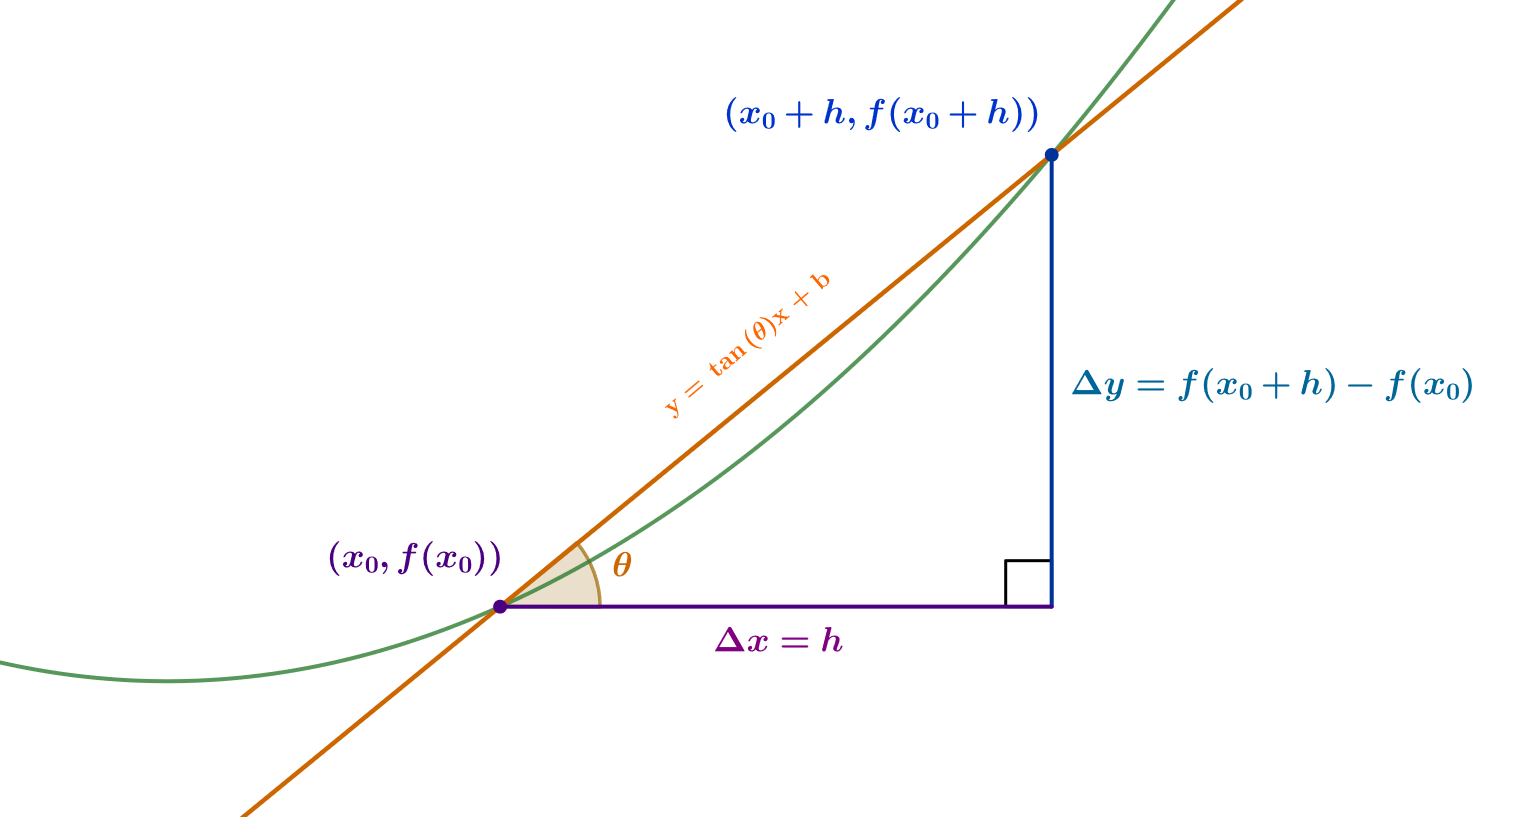
\includegraphics[scale=0.4]{definicja pochodna w punkcie.png}
\end{center}
\noindent Pochodną funkcji oznacza się: $f^{\prime}(x)$ (notacja Lagrange'a) lub $\frac{d}{d x} f$ (notacja Liebnitza).\hfill\break\\
\noindent Jeżeli we wzorze na pochodną zamiast granicy obustronnej badana będzie kolejno granica
prawostronna i lewostronna, to otrzymaną pochodną nazywa się odpowiednio pochodną prawostronną i pochodną lewostronną
funkcji $f$ w punkcie $x_{0}$. Pochodne te notuje się symbolicznie odpowiednio: $f^{\prime}_{+}(x)$, $f^{\prime}_{-}(x)$.\\

\subsection{Styczna do wykresu funkcji}
Niech funkcja $f$ będzie określona w pewnym sąsiedztwie punktu $x_{0}$ i różniczkowalna w tym punkcie.
Wtedy prostą styczną do wykresu funkcji $f$ w punkcie $x_{0}$ jest prosta o równaniu:
$$y = f^{\prime}(x_{0})(x - x_{0}) + f(x_{0})$$

\noindent Współczynnik kierunkowy stycznej do wykresu w punkcie $(x_{0}, f(x_{0}))$ jest równy tangensowi kąta nachylenia tej prostej do osi OX:

$$f^{\prime}(x) = \text{tg}(\alpha)$$

\noindent Normalna to prosta prostopadła do stycznej wykresu funkcji w punkcie $(x_{0}, f(x_{0}))$. Opisuje ją
równanie:
$$y = -\frac{1}{f^{\prime}(x_{0})}(x - x_{0}) + f(x_{0})$$

\subsection{Funkcja pochodna}
Niech $f$ będzie dowolną funkcją taką, że $f:X \rightarrow Y$. Funkcją pochodną funkcji $f$
nazywa się funkcję, która każdej liczbie $x_{0}$ należącej do dziedziny $X$ przyporządkowuje $f^{\prime}(x_{0})$, jeśli
pochodna w tym punkcie istnieje. Zbiór liczb z dziedziny funkcji $f$, dla których ta funkcja była różniczkowalna
jest dziedziną funkcji pochodnej.

\addcontentsline{toc}{subsection}{Pochodne wybranych funkcji}
{%

\renewcommand{\arraystretch}{2}
\renewcommand{\arraycolsep}{0.5cm}

\begin{center}
\begin{equation*}
\begin{array}{|c|c|c|c|}
\hline
f(x) & f^{\prime}(x) & f(x) & f^{\prime}(x)\\
\hline
 a & 0 & e^{x} & (x)^{\prime}e^{x} \\
 x & 1 & \log_{\;a}x & \dfrac{1}{x \ln a} \\
 ax^{n} & an\cdot x^{n-1} & \ln x & \dfrac{1}{x} \\
 \dfrac{1}{x} & -\dfrac{1}{x^{2}} & \sin x & \cos x \\
 \sqrt{x} & \dfrac{1}{2\sqrt{x}} & \cos x & -\sin x\\
 \sqrt[n]{x} & \dfrac{1}{n\sqrt[n]{x^{n-1}}} & \text{tg} x & \dfrac{1}{\cos^{2}x} = 1 + \text{tg}^{2} x \\
 a^{x} & (x)^{\prime}\cdot a^{x}\ln a & \text{ctg} x & -\dfrac{1}{\sin^{2}x} = -(1 + \text{ctg}^{2} x) \\[\medskipamount]
\hline
\end{array}
\end{equation*}
\end{center}
}%

\subsection{Własności pochodnych}
Niech funkcje $f$ i $g$ będą różniczkowalne w pewnym zbiorze $D$, będącym podzbiorem dziedzin
funkcji $f$ i $g$, a $\alpha$ i $\beta$ - dowolnymi liczbami rzeczywistymi. Wtedy dla dowolnej liczby $x \in D$:

{%
\renewcommand{\arraystretch}{2}

\begin{equation*}
\begin{array}{rcl}
   \displaystyle[\alpha f(x) + \beta g(x)]^{\prime} & = & \alpha f^{\prime}(x) + \beta g^{\prime}(x) \\
   \displaystyle[\alpha f(x) - \beta g(x)]^{\prime} & = & \alpha f^{\prime}(x) - \beta g^{\prime}(x) \\
   \displaystyle[\alpha \cdot f(x)\cdot g(x)]^{\prime} & = & \alpha (f^{\prime}(x) g(x) + f(x) g^{\prime}(x)) \\
   \displaystyle[\alpha \cdot f(x)]^{\prime} & = & \alpha \cdot f^{\prime}(x) \\
   \displaystyle\left[\frac{\alpha}{f(x)}\right]^{\prime} & = & -\dfrac{\alpha \cdot f^{\prime}(x)}{[f(x)]^{2}} \\[\medskipamount]
   \displaystyle\left[\frac{\alpha \cdot f(x)}{\beta \cdot g(x)}\right]^{\prime} & = & \dfrac{\alpha}{\beta} \left( \dfrac{ f^{\prime}(x) g(x) - f(x) g^{\prime}(x)}{[g(x)]^{2}}\right)\\
   \displaystyle [f(x)^{g(x)}]^{\prime} & = & f(x)^{g(x)}\left(g^{\prime}(x)\ln f(x) + \dfrac{f^{\prime}(x)g(x)}{f(x)}\right)
\end{array}   
\end{equation*}

}%

\noindent\textbf{Reguła łańcuchowa} - reguła pozwalająca obliczać pochodne funkcji złożonych.
Niech funkcje $f$ i $g$ będą funkcjami zmiennej rzeczywistej o wartościach rzeczywistych.
Jeżeli funkcja $f$ ma pochodną w punkcie $x_{0}$ oraz funkcja $g$ ma pochodną w punkcie $f(x_{0})$,
to wtedy funkcja złożona ma w punkcie $x_{0}$ pochodną:
$$(f\circ g)^{\prime}(x_{0}) = f^{\prime}(g(x_{0})) \cdot g^{\prime}(x_{0})$$
\textit{Przykład:}
$$\text{Wyznacz funkcję pochodną funkcji: }\sqrt{x^{2}-3}$$
$$f(x) = \sqrt{x},\;\; g(x) = x^{2}-3$$
$$\sqrt{x^{2}-3} = \sqrt{g(x)} = f(g(x)) = (f \circ g)(x)$$
\textit{Korzystając z reguły łańcuchowej:}
$$(\sqrt{x^{2}-3})^{\prime} = \left(\sqrt{g(x)}\right)^{\prime}\cdot g^{\prime}(x) = \frac{1}{2\sqrt{g(x)}} \cdot g^{\prime}(x) = $$
$$\frac{1}{2\sqrt{x^{2} - 3}} \cdot (x^{2}-3)^{\prime} = \frac{1}{2\sqrt{x^{2} - 3}} \cdot 2x \;\;=\;\; \frac{x}{\sqrt{x^{2} - 3}}$$

\subsection{Pochodna a monotoniczność funkcji}

Jeżeli funkcja $f$ ma pochodną w przedziale $(a, b)$ oraz dla każdej liczby rzeczywistej z tego przedziału:
\begin{itemize}
   \item $f^{\prime}(x) > 0$, to funkcja jest rosnąca w przedziale $(a, b)$;
   \item $f^{\prime}(x) \geq 0$, to funkcja jest niemalejąca w przedziale $(a, b)$;
   \item $f^{\prime}(x) = 0$, to funkcja jest stała w przedziale $(a, b)$;
   \item $f^{\prime}(x) \leq 0$, to funkcja jest nierosnąca w przedziale $(a, b)$;
   \item $f^{\prime}(x) < 0$, to funkcja jest malejąca w przedziale $(a, b)$.
\end{itemize}

Prawdziwe są twierdzenia odwrotne do powyższych.

\subsection{Ekstrema funkcji}
\noindent\textbf{Ekstremum funkcji} - maksymalna (maksimum) lub minimalna (minimum) wartość funkcji.\\
Wśród ekstrem rozróżnia się odpowiednie kategorie:
\begin{itemize}
   \item Maksimum (minimum) lokalne\\
   Punkt $x_{0}$ jest ekstremum lokalnym wtedy i tylko wtedy, gdy dla każdego punktu $x$ należącego jednocześnie do dziedziny funkcji $f$ oraz otoczenia punktu $x_{0}, U(x_{0})$
   prawdziwa jest nierówność:
   $$f(x) \leq f(x_{0}) \;\; (f(x) \geq f(x_{0}))$$
   Znaczy to, że w pewnej okolicy punktu $x_{0}$ nie występują wartości funkcji większe 
   (mniejsze) od wartości w punkcie $x_{0}$, choć mogą być tej wartości równe.\\

   \item Maksimum (minimum) lokalne właściwe\\
   Punkt $x_{0}$ jest ekstremum lokalnym właściwym wtedy i tylko wtedy, gdy dla każdego punktu $x$ należącego jednocześnie do dziedziny funkcji $f$ oraz otoczenia punktu $x_{0}, U(x_{0})$
   prawdziwa jest zależność:
   $$x = x_{0} \lor f(x) < f(x_{0}) \;\; (x = x_{0} \lor f(x) > f(x_{0}))$$
   Żadna wartość funkcji w otoczeniu punktu nie może być większa (mniejsza) ani równa wartości funkcji
   w punkcie $x_{0}$.\\
   
   \item Maksimum (minimum) globalne\\
   Punkt $x_{0}$ jest ekstremum globalnym wtedy i tylko wtedy, gdy dla każdego punktu $x$ w całej dziedzine funkcji $f$ prawdziwa jest nierówność:
   $$f(x) \leq f(x_{0}) \;\; (f(x) \geq f(x_{0}))$$
   W przeciwieństwie do ekstremum lokalnego, warunek dotyczy całej dziedziny.\\

   \item Maksimum (minimum) globalne właściwe\\
   Punkt $x_{0}$ jest ekstremum globalnym właściwym wtedy i tylko wtedy, gdy dla każdego punktu $x$ w całej dziedzine funkcji $f$ prawdziwa jest zależność:
   $$x = x_{0} \lor f(x) < f(x_{0}) \;\; (x = x_{0} \lor f(x) > f(x_{0}))$$
   W przeciwieństwie do ekstremum lokalnego właściwego, warunek dotyczy całej dziedziny.\\
\end{itemize}

\noindent\textbf{Punkt stacjonarny} - punkt w dziedzinie funkcji rzeczywistej, dla której pochodna tej
funkcji przyjmuje wartość równą zeru.\\

\noindent\textbf{Warunek konieczny istnienia ekstremum lokalnego (twierdzenie Fermata)} - dla różniczkowalnej funkcji $f$,
w pewnym przedziale $x_{0} \in (a, b)$, pochodna $f^{\prime}(x_{0}) = 0$.\\
Warunek Fermata nie gwarantuje istnienia ekstremów - funkcja może mieć pochodną równą zeru i nie mieć ekstremum
w tym punkcie, a może mieć ekstremum i nie mieć w nim pochodnej.\\

\noindent\textbf{Warunek konieczny i wystarczający ekstremum lokalnego} - dla różniczkowalnej, ciągłej funkcji $f: [a, b] \rightarrow \mathbb{R}$,
mającej skończoną ilość punktów stacjonarnych w punkcie $x_{0}$ istnieje
\begin{itemize}
   \item minimum lokalne wtedy i tylko wtedy, gdy istnieje $\delta > 0$ taka, że:
      \begin{itemize}
         \item $f^{\prime}(x_{0}) = 0$,
         \item $f^{\prime}(x_{0}) < 0 \text{ dla } x \in (x_{0} - \delta,\; x_{0})$,
         \item $f^{\prime}(x_{0}) > 0 \text{ dla } x \in (x_{0},\; x_{0} + \delta)$;
      \end{itemize}
   \hfill\break
   \item maksimum lokalne wtedy i tylko wtedy, gdy istnieje $\delta > 0$ taka, że:
      \begin{itemize}
         \item $f^{\prime}(x_{0}) = 0$,
         \item $f^{\prime}(x_{0}) > 0 \text{ dla } x \in (x_{0} - \delta,\; x_{0})$,
         \item $f^{\prime}(x_{0}) < 0 \text{ dla } x \in (x_{0},\; x_{0} + \delta)$.
      \end{itemize}
\end{itemize}

\noindent Alternatywnie, jeżeli funkcja $f$ jest dwukrotnie różniczkowalna w punkcie $x_{0} \in (a, b)$ i druga
pochodna jest ciągła, to jeżeli $f^{\prime}(x_{0}) = 0$ i $f^{\prime\prime}(x_{0}) \neq 0$, to funkcja
$f$ ma w punkcie $x_{0}$ ekstremum, przy czym jeżeli $f^{\prime\prime}(x_{0}) < 0$ to jest to maksimum
lokalne, a jeżeli $f^{\prime\prime}(x_{0}) > 0$ to jest to minimum lokalne.\\
Warunek ten nie rozstrzyga istnienia ekstremum, jeżeli druga pochodna jest równa 0.


\newpage

\section{Funkcje trygonometryczne}
\subsection{Miara łukowa kąta}
\InsertBoxR{0}{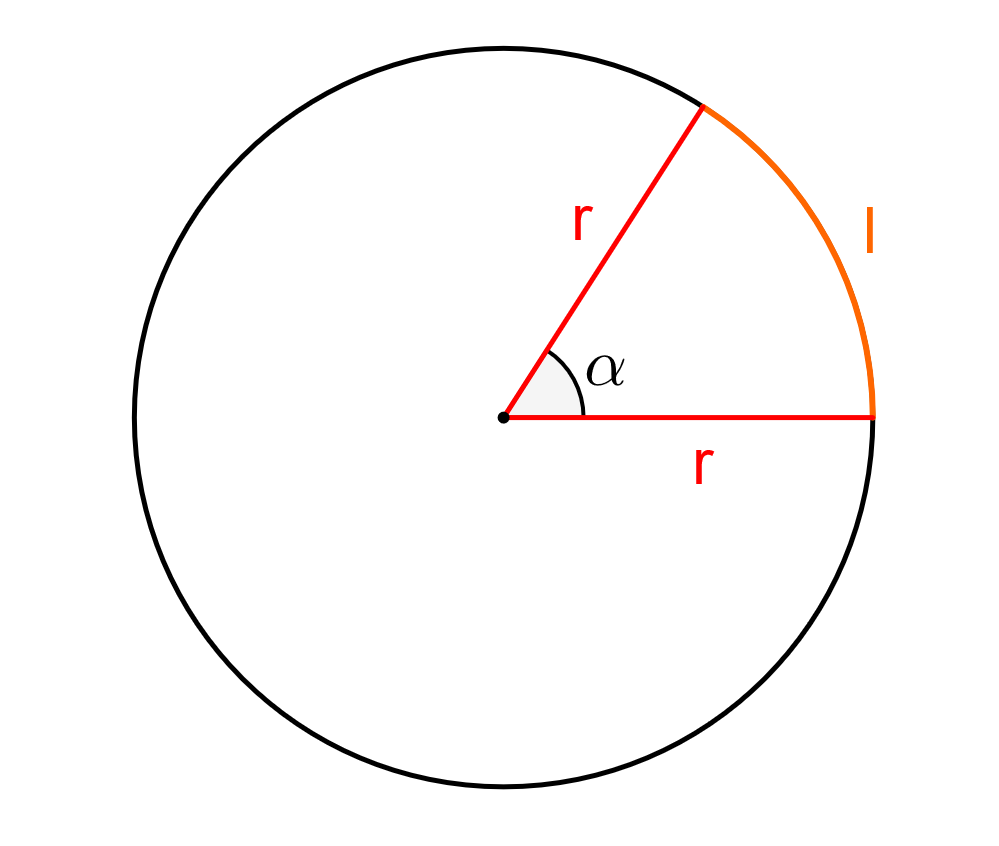
\includegraphics[scale=0.27]{trygonometria definicja radiany.png}}
\noindent Jednym ze sposobów podawania wartości kąta jest \textbf{radian} - Niemianowana jednostka
pochodna układu SI, zdefiniowana jako iloraz długości łuku nad długość promienia. Jeden radian to
długość łuku równa długości promienia.\\
$$\text{rad} = \dfrac{l}{r}$$\hfill\break
Zamiana miary:
\begin{itemize}
   \item stopniowej na łukową: $t^{\circ } = \dfrac{\pi \cdot t}{180} (\text{rad})$
   \item łukowej na stopniową: $t(\text{rad}) = \left(\dfrac{180 \cdot t}{\pi}\right)^{\circ}$
\end{itemize}
\subsection{Definicje funkcji trygonometrycznych}
\noindent\textbf{Definicja w trójkącie prostokątnym}


{%

\renewcommand{\arraystretch}{1.4}
%\renewcommand{\arraycolsep}{0.5cm}

%\textcolor{NavyBlue}
\begin{center}

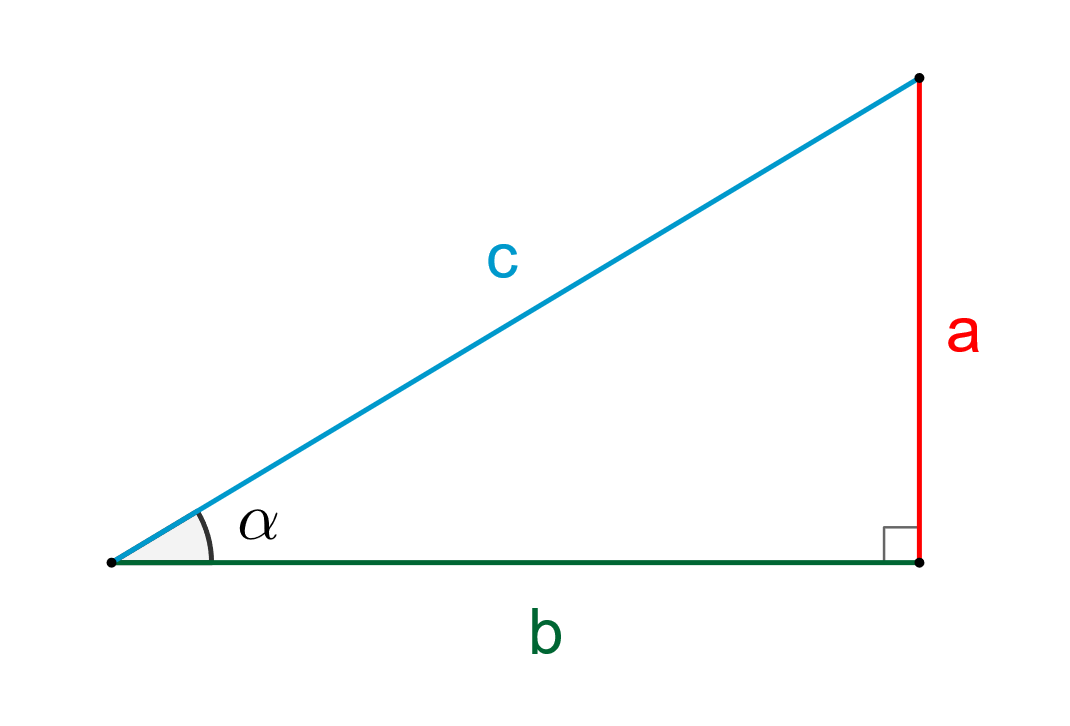
\includegraphics[scale=0.4]{trygonometria definicja w trójkącie.png}
\(\begin{array}{c|c|c}
   \sin \alpha = \dfrac{\textbfcolor{Red}{a}}{\textbfcolor{NavyBlue}{c}} & \text{tg}\; \alpha = \dfrac{\sin \alpha}{\cos \alpha} = \dfrac{\textbfcolor{Red}{a}}{\textbfcolor{OliveGreen}{b}} & \text{sec}\; \alpha = \dfrac{1}{\cos \alpha} = \dfrac{\textbfcolor{NavyBlue}{c}}{\textbfcolor{OliveGreen}{b}}\\[0.7cm]
   \cos \alpha = \dfrac{\textbfcolor{OliveGreen}{b}}{\textbfcolor{NavyBlue}{c}} & \text{ctg} \; \alpha = \dfrac{\cos \alpha}{\sin \alpha} = \dfrac{\textbfcolor{OliveGreen}{b}}{\textbfcolor{Red}{a}} & \text{cosec}\; \alpha = \dfrac{1}{\sin \alpha} = \dfrac{\textbfcolor{NavyBlue}{c}}{\textbfcolor{Red}{a}}
\end{array}\)  

\end{center}
\noindent\textbf{Definicja w okręgu jednostkowym (interpretacja geometryczna)}
\begin{center}

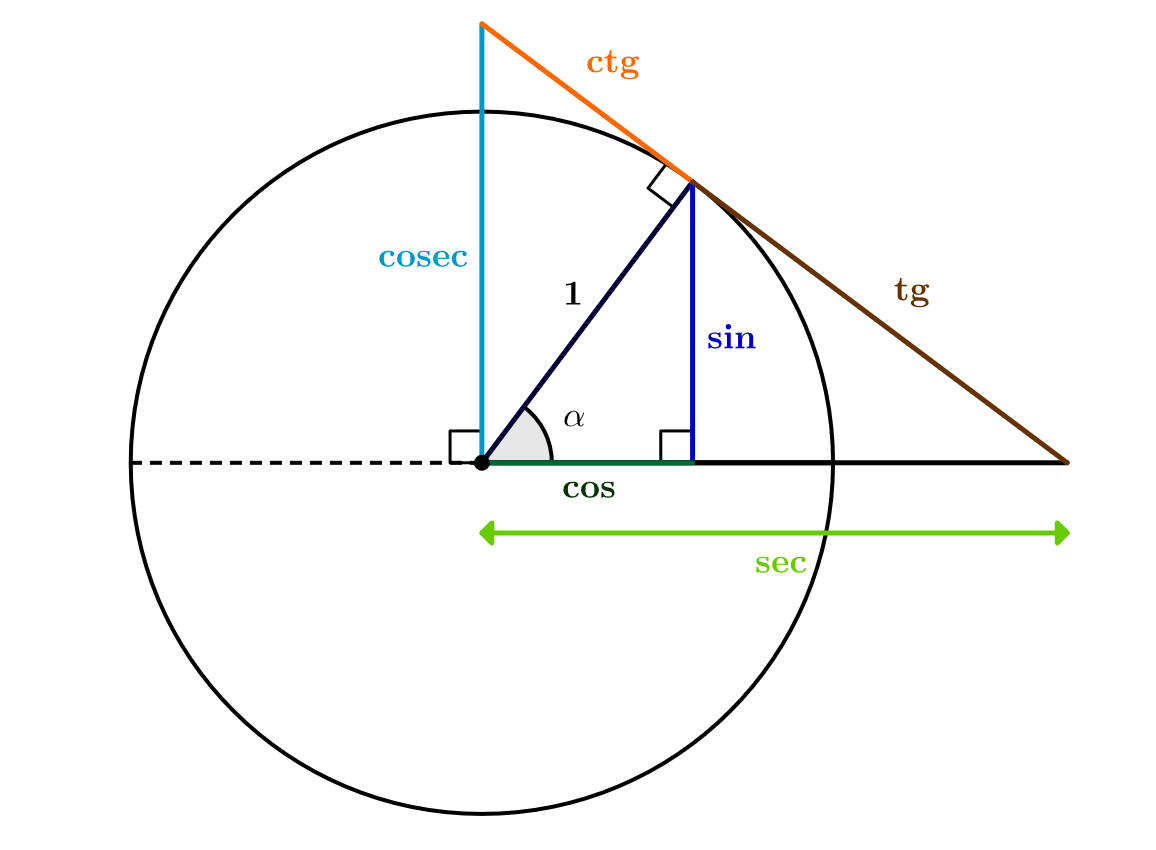
\includegraphics[scale=0.55]{trygonometria definicja w okręgu.png}

\end{center}
}%
\noindent Na powyższej ilustracji długości odcinków odpowiadają wartościom poszczególnych
funkcji trygonometrycznych względem kąta środkowego $\alpha$.\\

\noindent Dla wykresów funkcji trygonometrycznej, zobacz rozdział: \textit{4. Właściwości i wykresy funkcji - Wykresy funkcji, str. 22-23}.
\subsection{Podstawowe tożsamości trygonometryczne}

\begin{center}
{%
\renewcommand{\arraystretch}{2}
\renewcommand{\arraycolsep}{0.5cm}

\(
   \scalemath[1.3]{%
   \begin{array}{cc}
      \sin^{2} \alpha + \cos^{2} \alpha = 1 & \text{tg}\: \alpha \cdot \text{ctg}\: \alpha = 1\\
      \text{tg}^{2}\: \alpha + 1 = \text{sec}^{2}\: \alpha & \text{ctg}^{2}\: + 1 = \text{cosec}^{2}\: \alpha   
   \end{array}
   }%
\)

}%
\end{center}

\newpage

\subsection{Wartości funkcji trygonometrycznych}

\begin{center}
{%
\setlength\extrarowheight{10pt}

\(
\begin{array}{|c||c|c|c|c|c|c|c|}
   \hline
   \textbf{Radiany} & 0 & \dfrac{\pi}{12} & \dfrac{\pi}{6} & \dfrac{\pi}{4} & \dfrac{\pi}{3} & \dfrac{5\pi}{12} & \dfrac{\pi}{2}\\[0.1cm]
   \textbf{Stopnie} & 0^{\circ} & 15^{\circ} & 30^{\circ} & 45^{\circ} & 60^{\circ} & 75^{\circ} & 90^{\circ}\\[0.1cm]\hline\hline
   \scalemath[1.3]{\sin x} & 0 & \frac{\sqrt{6}-\sqrt{2}}{4} & \frac{1}{2} & \frac{\sqrt{2}}{2} & \frac{\sqrt{3}}{2} & \frac{\sqrt{6}+\sqrt{2}}{4} & 1 \\[0.3cm]\hline
   \scalemath[1.3]{\cos x} & 1 & \frac{\sqrt{6}+\sqrt{2}}{4} & \frac{\sqrt{3}}{2} & \frac{\sqrt{2}}{2} & \frac{1}{2} & \frac{\sqrt{6}-\sqrt{2}}{4} & 0 \\[0.3cm]\hline
   \scalemath[1.3]{\text{tg}\: x} & 0 & 2 - \sqrt{3} & \frac{\sqrt{3}}{3} & 1 & \sqrt{3} & 2 + \sqrt{3} & \scalemath[1.8]{\times} \\[0.3cm]\hline
   \scalemath[1.3]{\text{ctg}\: x} & \scalemath[1.8]{\times} & 2 + \sqrt{3} & \sqrt{3} & 1 & \frac{\sqrt{3}}{3} & 2 - \sqrt{3} & 0 \\[0.3cm]\hline
   \scalemath[1.3]{\text{sec}\: x} & 1 & \sqrt{6} - \sqrt{2} & \frac{2\sqrt{3}}{3} & \sqrt{2} & 2 & \sqrt{6} + \sqrt{2} & \scalemath[1.8]{\times} \\[0.3cm]\hline
   \scalemath[1.3]{\text{cosec}\: x} & \scalemath[1.8]{\times} & \sqrt{6} + \sqrt{2} & 2 & \sqrt{2} & \frac{2\sqrt{3}}{3} &  \sqrt{6} - \sqrt{2} & 1 \\[0.3cm]\hline
\end{array}
\)

}%
\end{center}

\subsection{Wzory redukcyjne}

\begin{center}
{%

\renewcommand{\arraystretch}{1.4}
\renewcommand{\arraycolsep}{0.15cm}
\setlength\extrarowheight{3pt}

\scalemath[0.9]{
\makebox[\linewidth]{
\(
\begin{array}{|c||c||c|c||c|c||c|c|}
      \hline
      {} & \textbf{I ćwiartka} & \multicolumn{2}{c||}{\textbf{II ćwiartka}} & \multicolumn{2}{c||}{\textbf{III ćwiartka}} & \multicolumn{2}{c|}{\textbf{IV ćwiartka}} \\[3pt]\hline\hline
      \multirow{2}{*}{$\varphi$} & 90^{\circ} - \alpha & 90^{\circ} + \alpha & 180^{\circ} - \alpha & 180^{\circ} + \alpha & 270^{\circ} - \alpha & 270^{\circ} + \alpha & 360^{\circ} - \alpha \\[3pt]\cline{2-8}
       ~ & \frac{1}{2}\pi - \alpha & \frac{1}{2}\pi + \alpha & \pi - \alpha & \pi + \alpha & \frac{3}{2}\pi - \alpha & \frac{3}{2}\pi + \alpha & 2\pi - \alpha \\[3pt]\hline\hline
      \sin \varphi & \cos \alpha & \cos \alpha & \sin \alpha & -\sin \alpha & -\cos \alpha & -\cos \alpha & -\sin \alpha \\[4pt]\hline
      \cos \varphi & \sin \alpha & -\sin \alpha & -\cos \alpha & -\cos \alpha & -\sin \alpha & \sin \alpha & \cos \alpha \\[4pt]\hline
      \tg \varphi & \ctg \alpha & -\ctg \alpha & -\tg \alpha & \tg \alpha & \ctg \alpha & -\ctg \alpha & -\tg \alpha \\[4pt]\hline
      \ctg \varphi & \tg \alpha & -\tg \alpha & -\ctg \alpha & \ctg \alpha & \tg \alpha & -\tg \alpha & -\ctg \alpha \\[4pt]\hline
      \sec \varphi & \cosec \alpha & -\cosec \alpha & -\sec \alpha & -\sec \alpha & -\cosec \alpha & \cosec \alpha & \sec \alpha \\[4pt]\hline
      \cosec \varphi & \sec \alpha & \sec \alpha & \cosec \alpha & -\cosec \alpha & -\sec \alpha & -\sec \alpha & -\cosec \alpha \\[4pt]\hline
\end{array}
% \begin{array}{|c||c|c||c|c||c|c||c|c|}
%       \hline
%       {} & \multicolumn{2}{c||}{\textbf{I ćwiartka}} & \multicolumn{2}{c||}{\textbf{II ćwiartka}} & \multicolumn{2}{c||}{\textbf{III ćwiartka}} & \multicolumn{2}{c|}{\textbf{IV ćwiartka}} \\[3pt]\hline\hline
%       \multirow{2}{*}{$\varphi$} & \multirow{2}{*}{$-\alpha$} & 90^{\circ} - \alpha & 90^{\circ} + \alpha & 180^{\circ} - \alpha & 180^{\circ} + \alpha & 270^{\circ} - \alpha & 270^{\circ} + \alpha & 360^{\circ} - \alpha \\[3pt]\cline{3-9}
%        ~ & ~ & \frac{1}{2}\pi - \alpha & \frac{1}{2}\pi + \alpha & \pi - \alpha & \pi + \alpha & \frac{3}{2}\pi - \alpha & \frac{3}{2}\pi + \alpha & 2\pi - \alpha \\[3pt]\hline\hline
%       \sin \varphi & -\sin \alpha & \cos \alpha & \cos \alpha & \sin \alpha & -\sin \alpha & -\cos \alpha & -\cos \alpha & -\sin \alpha \\[4pt]\hline
%       \cos \varphi & \cos \alpha & \sin \alpha & -\sin \alpha & -\cos \alpha & -\cos \alpha & -\sin \alpha & \sin \alpha & \cos \alpha \\[4pt]\hline
%       \tg \varphi & -\tg \alpha & \ctg \alpha & -\ctg \alpha & -\tg \alpha & \tg \alpha & \ctg \alpha & -\ctg \alpha & -\tg \alpha \\[4pt]\hline
%       \ctg \varphi & -\ctg \alpha & \tg \alpha & -\tg \alpha & -\ctg \alpha & \ctg \alpha & \tg \alpha & -\tg \alpha & -\ctg \alpha \\[4pt]\hline
%       \sec \varphi & \sec \alpha & \cosec \alpha & -\cosec \alpha & -\sec \alpha & -\sec \alpha & -\cosec \alpha & \cosec \alpha & \sec \alpha \\[4pt]\hline
%       \cosec \varphi & -\cosec \alpha & \sec \alpha & \sec \alpha & \cosec \alpha & -\cosec \alpha & -\sec \alpha & -\sec \alpha & -\cosec \alpha \\[4pt]\hline
% \end{array}
\)
}}
}%
\end{center}

\subsection{Tożsamości trygonometryczne}\hfill\break
\noindent\textbf{Funkcje trygonometryczne sumy i różnicy kątów}
\begin{center}
{%

%\renewcommand{\arraystretch}{1.4}
%\renewcommand{\arraycolsep}{0.15cm}
\setlength\extrarowheight{12pt}
\scalemath[0.9]{
\makebox[\linewidth]{
\(
\begin{array}{ll}
   \sin(\alpha + \beta) = \sin \alpha \cos \beta + \cos \alpha \sin \beta & \sin(\alpha - \beta) = \sin \alpha \cos \beta - \cos \alpha \sin \beta \\
   \cos(\alpha + \beta) = \cos \alpha \cos \beta - \sin \alpha \sin \beta & \cos(\alpha - \beta) = \cos \alpha \cos \beta + \sin \alpha \sin \beta \\[0.1cm]
   \text{tg}(\alpha + \beta) = \dfrac{\tg \alpha + \tg \beta}{1 - \tg \alpha \tg \beta} & \text{tg}(\alpha - \beta) = \dfrac{\tg \alpha - \tg \beta}{1 + \tg \alpha \tg \beta} \\[0.3cm]
   \text{ctg}(\alpha + \beta) = \dfrac{\ctg \alpha \ctg \beta - 1}{\ctg \beta + \ctg \alpha} & \text{ctg}(\alpha - \beta) = \dfrac{\ctg \alpha \ctg \beta + 1}{\ctg \beta - \ctg \alpha} \\[0.3cm]
   \sec(\alpha + \beta) = \dfrac{\sec \alpha \sec \beta \cosec \alpha \cosec \beta}{\cosec \alpha \cosec \beta - \sec \alpha \sec \beta} & \sec(\alpha - \beta) = \dfrac{\sec \alpha \sec \beta \cosec \alpha \cosec \beta}{\cosec \alpha \cosec \beta + \sec \alpha \sec \beta} \\[0.3cm]
   \text{cosec}(\alpha + \beta) = \dfrac{\sec \alpha \sec \beta \cosec \alpha \cosec \beta}{\cosec \alpha \cosec \beta + \sec \alpha \sec \beta} & \text{cosec}(\alpha - \beta) = \dfrac{\sec \alpha \sec \beta \cosec \alpha \cosec \beta}{\cosec \alpha \cosec \beta - \sec \alpha \sec \beta}
\end{array}
\)
}}

}%
\end{center}
\hfill\break\\

\noindent\textbf{Sumy i różnice funkcji trygonometrycznych}

\begin{center}
   {%
   
   %\renewcommand{\arraystretch}{1.4}
   %\renewcommand{\arraycolsep}{0.15cm}
   \setlength\extrarowheight{12pt}
   
   \scalemath[0.88]{
   \makebox[\linewidth]{
   \(
   \begin{array}{ll}
      \sin\alpha + \sin\beta = 2\sin\left(\dfrac{\alpha + \beta}{2}\right)\cos\left(\dfrac{\alpha - \beta}{2}\right) & \sin\alpha - \sin\beta = 2\sin\left(\dfrac{\alpha - \beta}{2}\right)\cos\left(\dfrac{\alpha + \beta}{2}\right) \\
      \cos\alpha + \cos\beta = 2\cos\left(\dfrac{\alpha + \beta}{2}\right)\cos\left(\dfrac{\alpha - \beta}{2}\right) & \cos\alpha - \cos\beta = -2\sin\left(\dfrac{\alpha + \beta}{2}\right)\sin\left(\dfrac{\alpha - \beta}{2}\right) \\[0.3cm]
      \text{tg}\:\alpha + \tg\beta = \dfrac{\sin(\alpha + \beta)}{\cos \alpha \cos \beta} & \text{tg}\:\alpha - \tg\beta = \dfrac{\sin(\alpha - \beta)}{\cos \alpha \cos \beta} \\[0.3cm]
      \text{ctg}\:\alpha + \ctg\beta = \dfrac{\sin(\beta + \alpha)}{\sin \alpha \sin \beta} & \text{ctg}\:\alpha - \ctg\beta = \dfrac{\sin(\beta - \alpha)}{\sin \alpha \sin \beta} \\[0.3cm]
      \text{tg}\:\alpha + \ctg\beta = \dfrac{\cos(\alpha - \beta)}{\cos \alpha \sin \beta} & \text{ctg}\:\alpha - \tg \beta = \dfrac{\cos(\alpha + \beta)}{\sin \alpha \cos \beta} \\
   \end{array}
   \)
   }}
   }%  
\end{center}

\newpage

\noindent\textbf{Funkcje trygonometryczne podwojonego i połowy kąta}

\begin{center}
{%
   
\renewcommand{\arraystretch}{1.2}
\renewcommand{\arraycolsep}{0.8cm}
\setlength\extrarowheight{11pt}
   
\makebox[\linewidth]{
\(
\begin{array}{ll}
   \sin(2\alpha) = 2\sin\alpha\cos\alpha & \cos(2\alpha) = \cos^{2}\alpha - \sin^{2}\alpha \\
   \cos(2\alpha) = 2\cos^{2}\alpha - 1 & \cos(2\alpha) = 1 - 2\sin^{2}\alpha \\
   \text{tg}(2\alpha) = \dfrac{2\tg\alpha}{1-\text{tg}^{2}\,\alpha} & \text{ctg}(2\alpha) = \dfrac{\text{ctg}^{2}\,\alpha - 1}{2\ctg\alpha} \\
   \sec(2\alpha) = \dfrac{\sec^{2}\alpha}{2 - \sec^{2} \alpha} & \text{cosec}(2\alpha) = \dfrac{\sec\alpha\cosec\alpha}{2} \\[1.3cm]
   \sin\left(\dfrac{\alpha}{2}\right) = \pm\sqrt{\dfrac{1-\cos\alpha}{2}} & \cos\left(\dfrac{\alpha}{2}\right) = \pm\sqrt{\dfrac{1+\cos\alpha}{2}} \\
   \text{tg}\left(\dfrac{\alpha}{2}\right) = \dfrac{\sin \alpha}{ 1 + \cos\alpha} & \text{ctg}\left(\dfrac{\alpha}{2}\right) = \dfrac{\sin \alpha}{ 1 - \cos\alpha}
\end{array}
\)
}
   
}%
\end{center}

\hfill\break\\

\noindent\textbf{Iloczyny funkcji trygonometrycznych}

\begin{center}
   {%
   
   %\renewcommand{\arraystretch}{1.4}
   %\renewcommand{\arraycolsep}{0.15cm}
   \setlength\extrarowheight{9pt}
   
   \makebox[\linewidth]{
   \(
   \begin{array}{ll}
      \sin\alpha\sin\beta = \dfrac{\cos(\alpha - \beta) - \cos(\alpha + \beta)}{2} & \cos\alpha\cos\beta = \dfrac{\cos(\alpha - \beta) + \cos(\alpha + \beta)}{2} \\[0.3cm]
      \sin\alpha\cos\beta = \dfrac{\sin(\alpha + \beta) + \sin(\alpha - \beta)}{2} & \text{tg}\:\alpha\tg\beta = \dfrac{\cos(\alpha - \beta) - \cos(\alpha + \beta)}{\cos(\alpha - \beta) + \cos(\alpha + \beta)} \\
   \end{array}
   \)
   }
   }%  
\end{center}

\hfill\break\\

\noindent\textbf{Redukcja potęg funkcji trygonometrycznych}

\begin{center}
   {%
   
   %\renewcommand{\arraystretch}{1.4}
   %\renewcommand{\arraycolsep}{0.15cm}
   \setlength\extrarowheight{9pt}
   
   \makebox[\linewidth]{
   \(
   \begin{array}{ll}
      \sin^{2}\alpha = \dfrac{1-\cos(2\alpha)}{2} & \cos^{2}\alpha = \dfrac{1 + \cos(2\alpha)}{2} \\[0.3cm]
      \sin^{2}\alpha\cos^{2}\alpha = \dfrac{1 - \cos(4\alpha)}{8} & \sin^{2}\alpha - \sin^{2}\beta = \sin(\alpha + \beta)\sin(\alpha - \beta) \\[0.3cm]
      \cos^{2}\alpha - \cos^{2}\beta = -\sin(\alpha + \beta)\sin(\alpha - \beta) & \cos^{2}\alpha - \sin^{2}\beta = \cos(\alpha + \beta)\cos(\alpha - \beta)\
   \end{array}
   \)
   }
   }%  
\end{center}

\subsection{Okresowość funkcji trygonometrycznych}
\noindent\textbf{Uwaga} - Funkcje $\arcsin(x)$, $\arccos(x)$, etc. to \textbf{funkcje cyklometryczne}, tj.
funkcje odwrotne do funkcji trygonometrycznych. W przeciwieństwie do zwykłej funkcji trygonometrycznej, to kąt
jest obrazem funkcji, podczas gdy wartość jest przeciwobrazem. Zachodzi więc następująca zależność:

\begin{center}

\(
\begin{array}{c}
   \sin(\alpha) = x \Leftrightarrow \arcsin(x) = \alpha,\\
   \cos(\alpha) = x \Leftrightarrow \arccos(x) = \alpha,\\
   \vdots 
\end{array}
\)
   
\end{center}

\noindent Dla poniższych definicji zakłada się, że $k \in \mathbb{C}$.\\

\noindent\textbf{Sinus} - $\sin: \mathbb{R} \rightarrow \langle-1, 1\rangle $ - okres podstawowy: $2\pi$

\begin{equation*}
   \sin\alpha = x \Leftrightarrow \left\{
      \begin{array}{ll}
         \begin{array}{l} 
         \!\!\!\!\alpha = \arcsin x + 2k\pi \\
         \!\!\!\!\alpha = \pi - \arcsin x + 2k\pi
         \end{array}\:, \; & x \in (-1, 0) \cup (0, 1) \\[0.6cm]
         \alpha = \dfrac{\pi}{2} + 2k\pi, & x = 1 \\[0.4cm]
         \alpha = k\pi, & x = 0 \\[0.4cm]
         \alpha = -\dfrac{\pi}{2} + 2k\pi, & x = -1 
      \end{array}
   \right.
\end{equation*}
\hfill\break\\
\noindent\textbf{Cosinus} - $\cos: \mathbb{R} \rightarrow \langle-1, 1\rangle $ - okres podstawowy: $2\pi$

\begin{equation*}
   \cos\alpha = x \Leftrightarrow \left\{
      \begin{array}{ll}
         \begin{array}{l} 
         \!\!\!\!\alpha = \arccos x + 2k\pi \\
         \!\!\!\!\alpha = - \arccos x + 2k\pi
         \end{array}\:, \; & x \in (-1, 0) \cup (0, 1) \\[0.6cm]
         \alpha = 2k\pi, & x = 1 \\[0.4cm]
         \alpha = \dfrac{\pi}{2} + k\pi, & x = 0 \\[0.4cm]
         \alpha = \pi + 2k\pi, & x = -1
      \end{array}
   \right.
\end{equation*}
\newpage
\noindent\textbf{Tangens} - $\tg\!: \mathbb{R}\setminus\left\{\alpha:\alpha=\dfrac{\pi}{2} + k\pi\right\} \rightarrow \mathbb{R} $ - okres podstawowy: $\pi$
\hfill\break\\
\begin{equation*}
   \!\!\!\!\!\!\!\!\!\!\!\!\!\!\!\!\!\!\!\!\!\!\!\!\!\!\!\!\!\!\!\!\!\!\!\!\tg\alpha = x \;\Leftrightarrow \left\{
      \begin{array}{ll}
         \alpha = k\pi, & x = 0 \\[0.4cm]
         \alpha = \text{arctg}\:x + k\pi, & x \in \mathbb{R}\setminus\{0\}
      \end{array}
   \right.
\end{equation*}
\hfill\break\\
\noindent\textbf{Cotangens} - $\ctg\!: \mathbb{R}\setminus\left\{\alpha:\alpha=k\pi\right\} \rightarrow \mathbb{R} $ - okres podstawowy: $\pi$
\hfill\break\\
\begin{equation*}
   \!\!\!\!\!\!\!\!\!\!\!\!\!\!\!\!\!\!\!\!\!\!\!\!\!\!\!\!\!\!\!\!\!\!\!\!\tg\alpha = x \;\Leftrightarrow \left\{
      \begin{array}{ll}
         \alpha = \dfrac{\pi}{2} + k\pi, & x = 0 \\[0.4cm]
         \alpha = \text{arcctg}\:x + k\pi, & x \in \mathbb{R}\setminus\{0\}
      \end{array}
   \right.
\end{equation*}
\hfill\break\\
\noindent\textbf{Secans} - $\sec: \mathbb{R}\setminus\left\{\alpha:\alpha=\dfrac{\pi}{2} + k\pi\right\} \rightarrow (-\infty, -1\rangle \cup \langle 1, +\infty) $ - okres podstawowy: $2\pi$
\hfill\break\\
\noindent\textbf{Cosecans} - $\cosec: \mathbb{R}\setminus\left\{\alpha:\alpha=k\pi\right\} \rightarrow (-\infty, -1\rangle \cup \langle 1, +\infty) $ - okres podstawowy: $2\pi$

\newpage

\section{Planimetria}
\begin{center}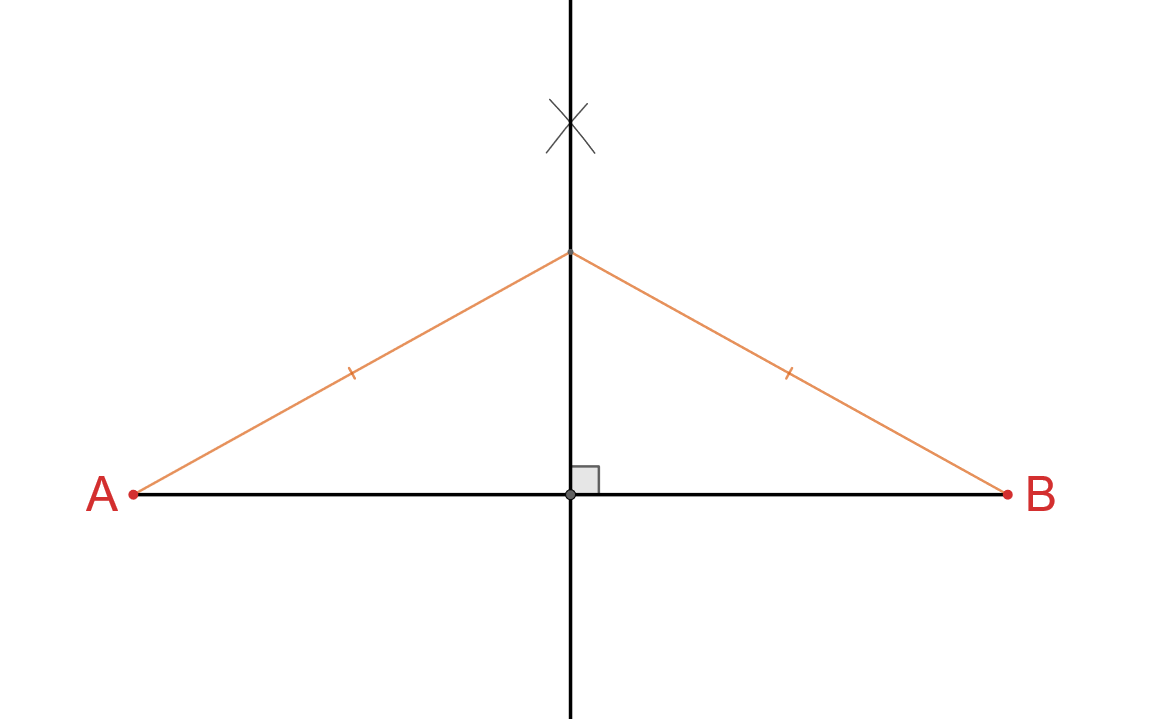
\includegraphics[scale=0.5]{geometria/symetralna odcinka.png}\end{center}
\addcontentsline{toc}{subsection}{Symetralna odcinka}
\noindent \textbf{Symetralna odcinka} - jest to prosta prostopadła do odcinka, która dzieli ten odcinek
na dwie równe części. Symetralna jest też zbiorem wszystkich punktów równo odległych od punktów na końcach
odcinka.\\
\InsertBoxR{0}{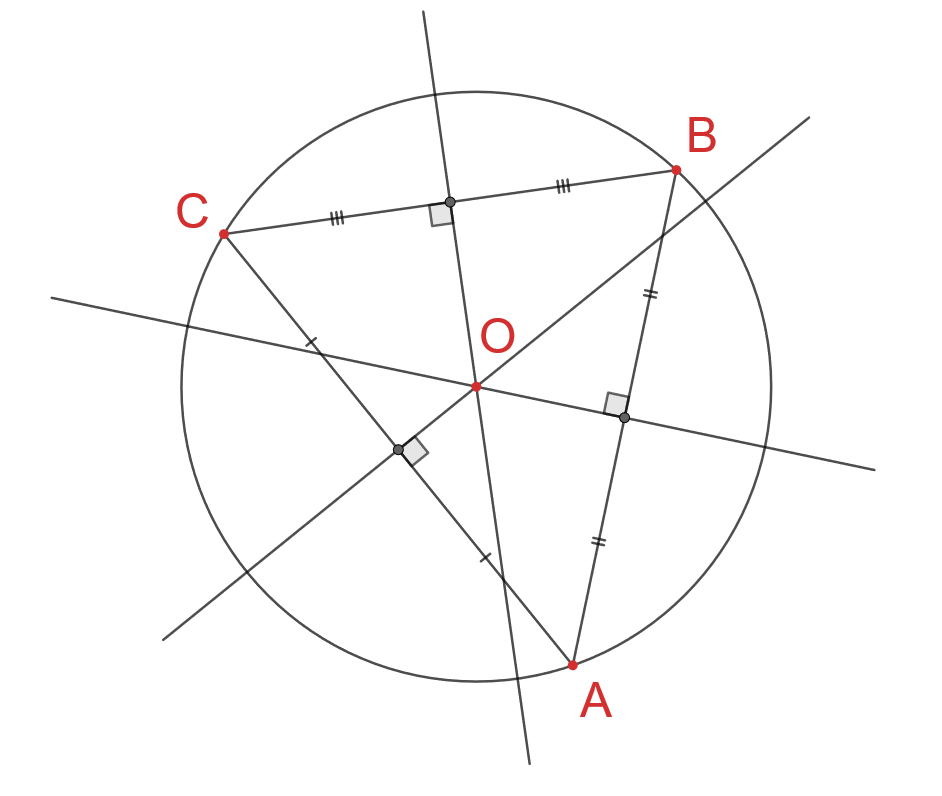
\includegraphics[scale=0.35]{geometria/środek okręgu opisanego.png}}
\noindent Aby skonstruować symetralną, należy zakreślić dwa półokręgi, o równych promieniach większych od połowy długości
odcinka, a następnie połączyć prostą punkty przecięć tych półokręgów.\\\\
\noindent Symetralne trzech boków dowolnego trójkąta przecinają się w punkcie, który jest środkiem okręgu opisanego
na trójkącie (częściami wspólnymi okręgu i trójkąta są wierzchołki trójkąta).

\begin{center}\includegraphics[scale=0.5]{geometria/dwusieczna kąta.png}\end{center}
\addcontentsline{toc}{subsection}{Dwusieczna kąta}
\noindent \textbf{Dwusieczna kąta} - półprosta o początku w wierzchołku kąta, która dzieli kąt zawarty
między ramionami kąta na dwa równe kąty, każdy o mierze równej połowie oryginalnego kąta. Dwusieczna kąta
jest zbiorem punktów równo odległych od ramion kąta wypukłego.\\\MoveBelowBox\unskip

\InsertBoxR{0}{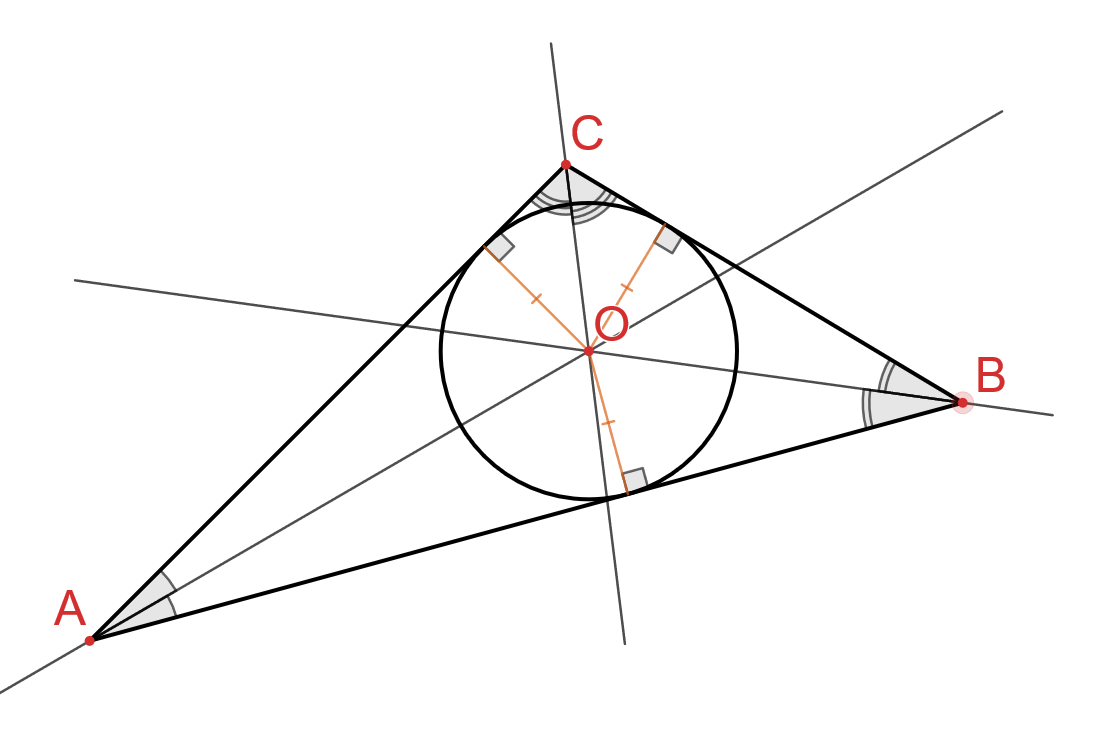
\includegraphics[scale=0.34]{geometria/środek okręgu wpisanego.png}}
\noindent By skonstuować dwusieczną, należy zakreślić półokrąg o środku w punkcie A. Następnie
z miejsc przecięcia się ramion kąta i półokręgu zakreślić kolejne półokręgi o promieniu większym niż
połowa odległości do drugiego punktu przecięcia. Dwusieczna to prosta przechodząca przez punkt przecięcia 
dwóch półokręgów i punkt A.\\

\noindent Dwusieczne trzech kątów dowolnego trójkąta przecinają się w punkcie, który jest środkiem okręgu
wpisanego w trójkąt (częściami wspólnymi okręgu i trójkąta są trzy punkty, każdy należy do innego boku).

\begin{center}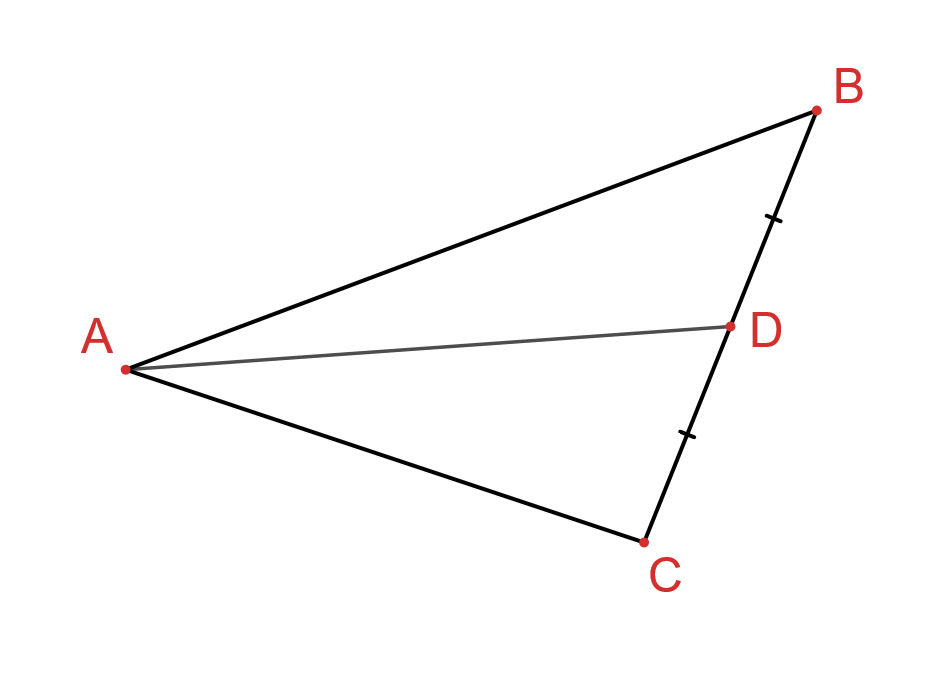
\includegraphics[scale=0.5]{geometria/środkowa trójkąta.png}\end{center}
\addcontentsline{toc}{subsection}{Środkowa trójkąta}
\noindent \textbf{Środkowa trójkąta} - odcinek łączący wierzchołek trójkąta z środkiem przeciwległego boku.\\
% Długość środkowej $d$, opadającej na bok $c$ można obliczyć ze wzoru:\hfill\break
% \begin{center}
% \(
% d = \dfrac{1}{2}\sqrt{2a^{2}+2b^{2}-c^{2}}
% \)

% \end{center}\unskip
\MoveBelowBox\unskip

\InsertBoxR{0}{\includegraphics[scale=0.33]{geometria/środkowe.png}}
\noindent W dowolnym trójkącie trzy środkowe przecinają się w jednym punkcie (barycentrum, środek ciężkości trójkąta), który to dzieli każdą
z środkowych na fragmenty o długości w stosunku 2:1, licząc od wierzchołka trójkąta.\\\\
Każdy z sześciu trójkątów ograniczonych środkowymi trójkąta ma to samo pole.

\MoveBelowBox
\noindent \textbf{Twierdzenie o środkowej (twierdzenie Apolloniusza)} - suma kwadratów dwóch dowolnych
boków jest równa podwojonej sumie kwadratów połowy trzeciego boku i środkowej opartej na trzecim boku.\\
Jeżeli boki trójkątu to $a, b, c$, a $d$ to środkowa oparta na boku $c$, to wtedy:
$$a^{2}+b^{2} = 2\left(\left(\frac{1}{2}c\right)^{2} + d^{2}\right)$$

\newpage

\addcontentsline{toc}{subsection}{Twierdzenie o dwusiecznej kąta wewnętrznego}
\begin{center}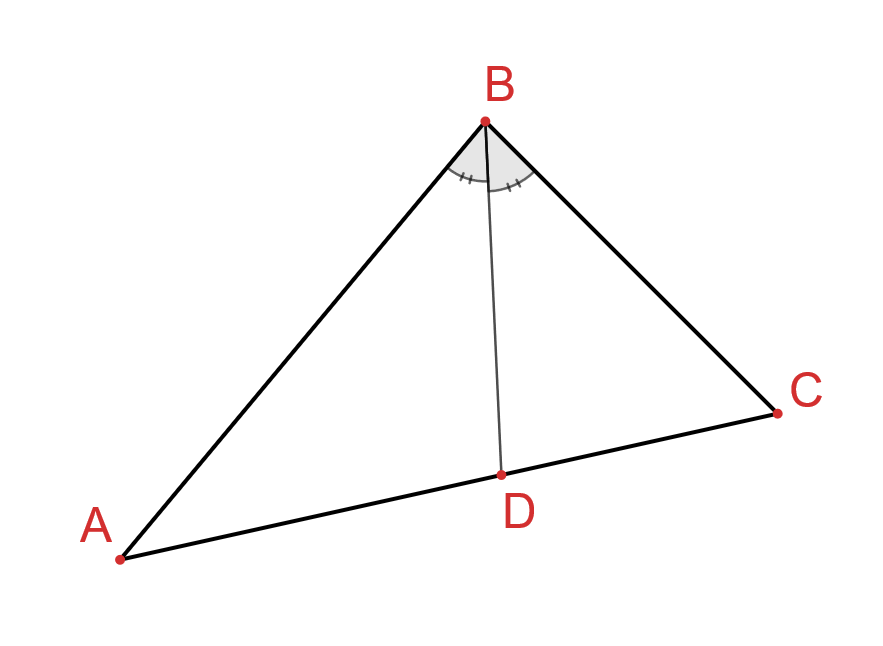
\includegraphics[scale=0.5]{geometria/odcinki w trójkącie zdwusiecznionym.png}\end{center}
\noindent \textbf{Twierdzenie o dwusiecznej kąta wewnętrznego} - w dowolnym trójkącie $ABC$, w którym
odcinek $\vert BD\vert$ jest dwusieczną kąta wewnętrznego, prawdziwa jest równość:

$$\dfrac{\vert AB\vert}{\vert BC\vert} = \dfrac{\vert AD\vert}{\vert DC\vert}$$

\hfill\break \addcontentsline{toc}{subsection}{Nierówność w trójkącie}
\noindent\textbf{\!\!Nierówność w trójkącie} - W dowolnym trójkącie suma długości dwóch dowolnych boków jest
większa od długości trzeciego boku.\MoveBelowBox\unskip

\InsertBoxL{0}{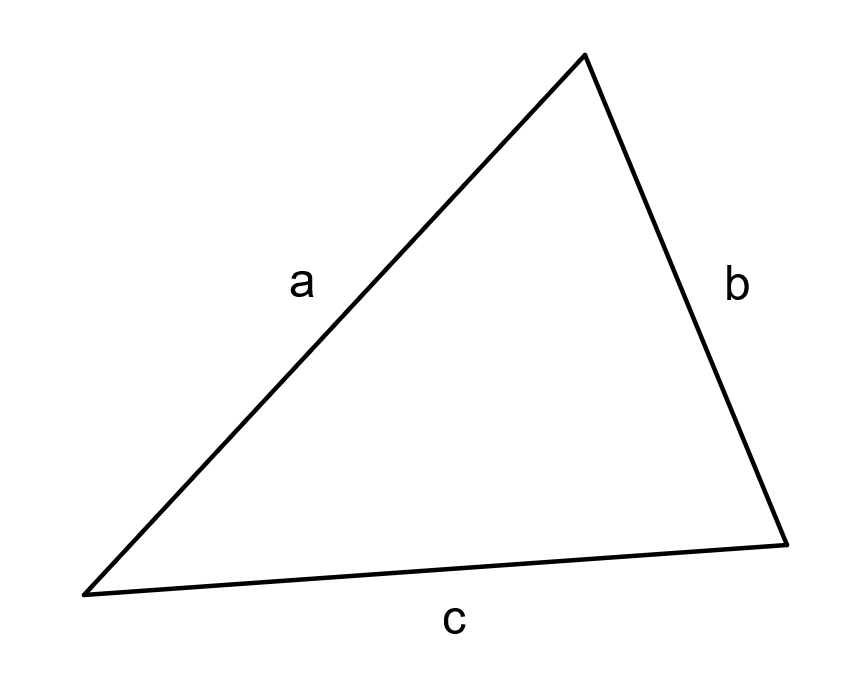
\includegraphics[scale=0.3]{geometria/nirówność trójkąta.png}}
{%
   \renewcommand{\arraystretch}{1.4}
   %\renewcommand{\arraycolsep}{0.15cm}
   \setlength\extrarowheight{9pt}
\begin{center}
   \begin{tabular}{>{\hspace{7cm}}c}
      $a + b > c$\\
      $a + c > b$\\
      $b + c > a$
   \end{tabular}   
\end{center}
}%
\MoveBelowBox

\newpage

\subsection{Twierdzenie Pitagorasa}
\noindent Jeżeli trójkąt jest prostokątny, to wtedy suma kwadratów długości przyprostokątnych $a$ i $b$
jest równa kwadratowi przeciwprostokątnej $c$:
$$\text{Trójkąt prostokątny} \Leftrightarrow a^{2} + b^{2} = c^{2}$$\hfill\break
\noindent Z twierdzenia Pitagorasa wynika również, że jeżeli trójkąt jest ostrokątny, to wtedy suma kwadratów
dwóch krótszych boków jest większa od kwadratu najdłuższego boku:
$$\text{Trójkąt ostrokątny} \Leftrightarrow a^{2} + b^{2} > c^{2}$$\hfill\break
\noindent Jeżeli trójkąt jest rozwartokątny, to wtedy suma kwadratów
dwóch krótszych boków jest mniejsza od kwadratu najdłuższego boku:
$$\text{Trójkąt rozwartokątny} \Leftrightarrow a^{2} + b^{2} < c^{2}$$\hfill\break
Twierdzenia odwrotne do powyższych również są prawdziwe.

\subsection{Twierdzenie Steinera-Lehmusa}
\begin{center}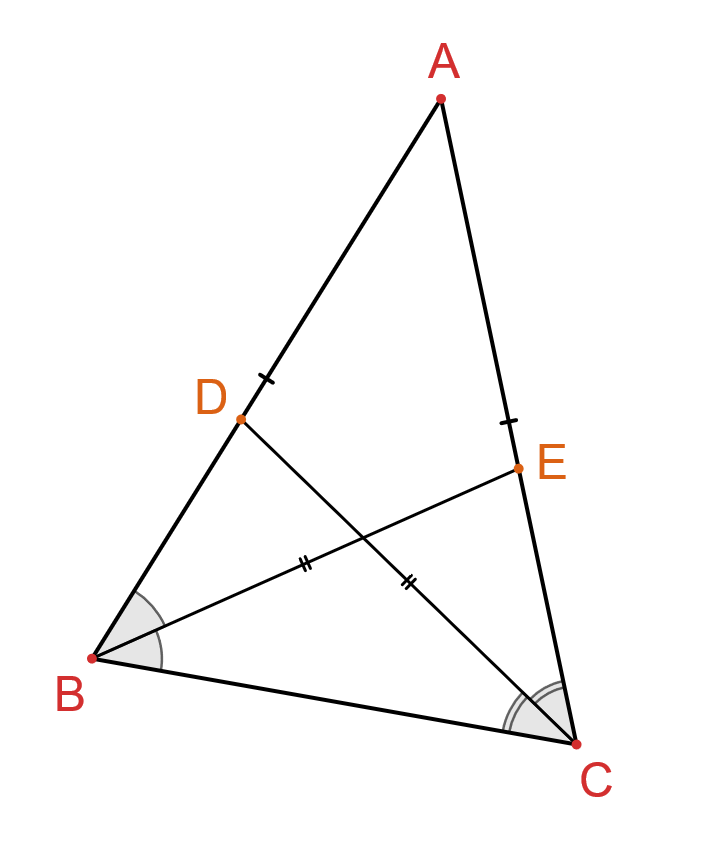
\includegraphics[scale=0.4]{geometria/twierdzenie Steinera-Lehmusa.png}\end{center}
\noindent Jeżeli w trójkącie istnieją dwa równe odcinki które są dwusiecznymi dwóch różnych jego kątów wewnętrznych,
to wtedy rzeczony trójkąt jest równoramienny.

\subsection{Pole trójkąta - wzory}
\begin{center}\includegraphics[scale=0.5]{geometria/pole trójkąta.png}\end{center}

\begin{center}
{%
\renewcommand{\arraystretch}{1.4}
%\renewcommand{\arraycolsep}{0.15cm}
\setlength\extrarowheight{9pt}

   \scalemath[1.2]{
   \makebox[\linewidth]{
   \(
   \begin{array}{ll}
      \hspace{-2cm}P = \dfrac{1}{2}ch & P = \dfrac{1}{2}bc \cdot \sin \alpha\\
      \hspace{-2cm}P = \dfrac{b^{2}}{2(\ctg\alpha + \ctg\gamma)} & P = p\cdot r,\;\; p = \dfrac{a + b + c}{2} \\
      \hspace{-2cm}P = \sqrt{p(p-a)(p-b)(p-c)} & P = \dfrac{abc}{4R} \\
      \multicolumn{2}{c}{\hspace{-2cm}P = \dfrac{1}{4}\text{tg}\:\alpha(b^{2}+c^{2}-a^{2})}\\
   \end{array}   
   \) 
   }}
}%
\end{center}

\subsection{Promień okręgu wpisanego i opisanego dowolnego trójkąta}
\begin{center}
   {%
   \renewcommand{\arraystretch}{1.4}
   %\renewcommand{\arraycolsep}{0.15cm}
   \setlength\extrarowheight{9pt}
   
      \scalemath[1.2]{
      \makebox[\linewidth]{
      \(
      \begin{array}{>{\hspace{-3cm}}c}
         R = \sqrt{\dfrac{a^{2}b^{2}c^{2}}{(a+b+c)(-a+b+c)(a-b+c)(a+b-c)}} \\[1cm]
         r = \sqrt{\dfrac{(-a+b+c)(a-b+c)(a+b-c)}{4(a+b+c)}}
      \end{array}   
      \) 
      }}
   }%
\end{center}

\subsection{Twierdzenia o dowolnych trójkątach}

\InsertBoxR{0}{\includegraphics[scale=0.3]{geometria/twierdzenie Cevy.png}}
\hfill\break
\noindent \textbf{Twierdzenie Cevy} - niech dany będzie trójkąt $ABC$ i punkty $D, E, F$ takie, że
$D \in \vert BC\vert$, $E \in \vert AC\vert$ i $F \in \vert AB\vert$. Jeżeli proste $\vert AD\vert, \vert BE\vert$ i
$\vert CF\vert$ przecinają się w jednym punkcie $O$, to wtedy prawdziwa jest równość:
$$\dfrac{\vert AF\vert}{\vert FB\vert} \cdot \dfrac{\vert BD\vert}{\vert DC\vert} \cdot \dfrac{\vert CE\vert}{\vert EA\vert} = 1$$
\MoveBelowBox\unskip
\hfill\break

\InsertBoxR{0}{\includegraphics[scale=0.32]{geometria/twierdzenie Eulera.png}}
\hfill\break
\noindent \textbf{Twierdzenie Eulera} - twierdzenie opisujące relację między długościami promieni
okręgów: wpisanego w i opisanego na trójkącie a odległością między środkami tych okręgów.\\
Długość odcinka $d$, będącego odległością środków okręgów: wpisanego i opisanego jest równa:
$$d^{2} = R(R-2r)$$
Z twierdzenia tego wynika również \textbf{nierówność Eulera}: $R \geq 2r$
\MoveBelowBox\unskip
\hfill\break

\InsertBoxR{0}{\includegraphics[scale=0.32]{geometria/twierdzenie o trójliściu.png}}
\hfill\break
\noindent \textbf{Twierdzenie o trójliściu} - niech dany będzie dowolny trójkąt $ABC$. Prosta $BO_{r}$,
przechodząca przez wierzchołek trójkąta i środek okręgu wpisanego w ten trójkąt przecina okrąg 
opisany na trójkącie w punkcie $D$. W takiej konfiguracji prawdziwa jest równość:
$$\vert AD\vert = \vert O_{r}D\vert = \vert CD \vert$$

\newpage
\MoveBelowBox\unskip
\hfill\break

\InsertBoxR{0}{\includegraphics[scale=0.29]{geometria/połączone środki boków trójkąta.png}}
\hfill\break
\noindent \textbf{Twierdzenie o linii środkowej} - linia środkowa (odcinek łączący środki
dwóch boków trójkąta) jest równoległa do odpowiadającego
jej boku oraz długość linii środkowej jest równa połowie długości odpowiadającego boku.
$$\vert DE\vert = \dfrac{1}{2}\vert AB\vert$$
\hfill\break

\InsertBoxR{0}{\includegraphics[scale=0.29]{geometria/twierdzenie Routha.png}}
\hfill\break
\noindent \textbf{Twierdzenie Routha} - opisuje stosunek między polami trójkąta i trójkąta zawartego
między czewianami (dowolnymi odcinkami łączącymi wierzchołek trójkąta i przeciwległy bok).\\\\
Niech dany będzie dowolny trójkąt $ABC$ i $D \in \vert BC\vert$, $E \in \vert AC\vert$ i $F \in \vert AB\vert$.
Wiedząc, że $x = \frac{\vert CD\vert}{\vert BD\vert}$, $y = \frac{\vert AE\vert}{\vert CE\vert}$ i
$z = \frac{\vert BF\vert}{\vert AF\vert}$ pole trójkąta $GHI$ jest równe polu trójkąta $ABC$ razy:
$$\dfrac{(xyz - 1)^{2}}{(xy + y +1)(yz + z + 1)(zx + x + 1)}$$

\newpage

\subsection{Trójkąt równoboczny - wzory}
\begin{center}\includegraphics[scale=0.5]{geometria/trójkąt równoboczny.png}\end{center}
\begin{center}
   {%
   \renewcommand{\arraystretch}{1.4}
   \renewcommand{\arraycolsep}{0.5cm}
   \setlength\extrarowheight{9pt}
   
      \scalemath[1.2]{
      \makebox[\linewidth]{
      \(
         \begin{array}{>{\hspace{-3cm}}ll}
            P = \dfrac{a^{2}\sqrt{3}}{4} & h = \dfrac{a\sqrt{3}}{2} \\
            R = \dfrac{2}{3}h = \dfrac{a\sqrt{3}}{3} & r = \dfrac{1}{3}h = \dfrac{a\sqrt{3}}{6} \\
         \end{array}
      \) 
      }}
   }%
\end{center}
\newpage
\MoveBelowBox\unskip

\subsection{Twierdzenia o trójkątach równobocznych}

\InsertBoxR{0}{\includegraphics[scale=0.3]{geometria/twierdzenie Vivianiego.png}}
\hfill\break
\noindent \textbf{Twierdzenie Vivianiego} - Dla każdego punktu wewnątrz trójkąta równobocznego suma odległości tego punktu
od boków trójkąta jest równa jego wysokości.

\MoveBelowBox
\hfill\break
\InsertBoxR{0}{\includegraphics[scale=0.28]{geometria/twierdzenie Van Schootena.png}}
\hfill\break
\noindent \textbf{Twierdzenie Van Schootena} - Dla punktu $D$ umieszczonego na okręgu opisanym na trójkącie równobocznym długość najdłuższego
odcinka łączącego ten punkt z wierzchołkiem jest równa sumie długości dwóch pozostałych odcinków łączących
punkt $D$ z pozostałymi wierzchołkami.\\

\noindent Jest to specjalny przypadek \textbf{twierdzenia \linebreak M\"obiusa - Pompejusza} które postuluje, że odcinki łączące dowolny
punkt $D$ na płaszczyźnie z wierzchołkami trójkąta równobocznego spełniają nierówność trójkąta (da się
z nich zbudować trójkąt).

\newpage
\subsection{Trójkąt prostokątny - wzory}
\begin{center}\includegraphics[scale=0.5]{geometria/trójkąt prostokątny 2.png}\end{center}
\begin{center}
   {%
   \renewcommand{\arraystretch}{1.4}
   \renewcommand{\arraycolsep}{0.5cm}
   \setlength\extrarowheight{9pt}
   
      \scalemath[1.2]{
      \makebox[\linewidth]{
      \(
         \begin{array}{>{\hspace{-3cm}}ll}
            P = \dfrac{1}{2}ab & h = \sqrt{ef} \\
            a = \sqrt{ce} & b = \sqrt{cf} \\
            r = \dfrac{a + b - c}{2} & R = \dfrac{1}{2}c

         \end{array}
      \) 
      }}
   }%
\end{center}
\hfill\break
\noindent \textbf{Twierdzenie Talesa o kącie wpisanym} - jeżeli jeden z boków trójkąta jest średnicą
okręgu na nim opisanego, to wtedy jest to trójkąt prostokątny, a średnica jest przeciwprostokątną.

\newpage

\subsection{Cechy przystawania trójkątów}
\noindent \textbf{I cecha przystawania trójkątów (bbb)}
\begin{center}\includegraphics[scale=0.45]{geometria/przystawanie bbb.png}\end{center}
$$a=a_{1} \land b=b_{1} \land c=c_{1} \Rightarrow ABC \equiv A_{1}B_{1}C_{1}$$
\noindent Jeżeli długości trzech boków w jednym trójkącie są odpowiednio równe długościom trzech boków
w drugim trójkącie, to wtedy te trójkąty są przystające.\\\\
\noindent \textbf{II cecha przystawania trójkątów (bkb)}
\begin{center}\includegraphics[scale=0.45]{geometria/przystawanie bkb.png}\end{center}
$$b=b_{1}\land \alpha = \alpha_{1} \land c=c_{1} \Rightarrow ABC \equiv A_{1}B_{1}C_{1}$$
Jeżeli dwa boki i kąt między tymi bokami w jednym trójkącie są odpowiednio równe dwóm bokom i kątowi
między tymi bokami w drugim trójkącie, to te trójkąty są przystające.\\\\
\noindent \textbf{III cecha przystawania trójkątów (kbk)}
\begin{center}\includegraphics[scale=0.45]{geometria/przystawanie kbk.png}\end{center}
$$\alpha = \alpha_{1}\land b=b_{1}\land \beta=\beta_{1} \Rightarrow ABC \equiv A_{1}B_{1}C_{1}$$
Jeżeli bok i dwa przyległe do niego kąty w jednym trójkącie są odpowiednio równe bokowi i dwóm
przyległym do niego kątom w drugim trójkącie, to wtedy te trójkąty są przystające.

\newpage

\subsection{Cechy podobieństwa trójkątów}
\noindent \textbf{Cecha podobieństwa trójkątów (kkk)}
\begin{center}\includegraphics[scale=0.4]{geometria/podobieństwo kkk.png}\end{center}
$$\alpha = \delta \land \beta = \gamma \Rightarrow ABC \sim DEF$$
Jeżeli dwa kąty jednego trójkąta są odpowiednio równe dwóm kątom drugiego trójkąta, to trójkąty te są
podobne.\\\\
\noindent \textbf{Cecha podobieństwa trójkątów (bbb)}
\begin{center}\includegraphics[scale=0.4]{geometria/podobieństwo bbb.png}\end{center}
$$\dfrac{d}{a} = \dfrac{e}{b} = \dfrac{f}{c} = k, \text{ gdzie } k \text{ - skala podobieństwa} \Rightarrow ABC \sim DEF$$
Jeżeli długości boków jednego trójkąta są proporcjonalne do odpowiednich długości boków drugiego trójkąta,
to trójkąty te są podobne.\\\\
\noindent \textbf{Cecha podobieństwa trójkątów (bkb)}
\begin{center}\includegraphics[scale=0.4]{geometria/podobieństwo bkb.png}\end{center}
$$\dfrac{e}{b} = \dfrac{f}{c} = k, \text{ gdzie } k \text{ - skala podobieństwa} \land \alpha = \delta \Rightarrow ABC \sim DEF$$
Jeżeli długości dwóch boków jednego trójkąta są proporcjonalne do odpowiednich długości boków drugiego
trójkąta oraz kąty między tymi bokami są równe, to trójkąty te są podobne.\\\\
Jeżeli trójkąty $T_{1}, T_{2}$ są podobne w skali $k$, to stosunek pól tych trójkątów jest równy
kwadratowi skali podobieństwa.

\subsection{Twierdzenie sinusów}
W dowolnym trójkącie iloraz długości dowolnego boku i sinusa kąta leżącego naprzeciwko tego boku jest
równy średnicy okręgu opisanego:
\begin{center}
\scalemath[1.2]{
\makebox[\linewidth]{
   \(
      \hspace{-3cm}\dfrac{a}{\sin \alpha} = \dfrac{b}{\sin \beta} = \dfrac{c}{\sin \gamma} = 2R
   \)
}}
\end{center}
\newpage

\subsection{Twierdzenie cosinusów}
W dowolnym trójkącie kwadrat długości dowolnego boku jest równy sumie kwadratów długości pozostałych boków
pomniejszonej o podwojony iloczyn długości tych boków i cosinusa kąta zawartego między nimi.
\begin{center}
   \scalemath[1.2]{
   \makebox[\linewidth]{
   \(
   \hspace{-2.7cm}a^{2} = b^{2} + c^{2} - 2bc\cos \alpha
   \)
   }}
\end{center}

\subsection{Twierdzenie tangensów}
W dowolnym trójkącie, jeżeli $a, b$ to miary dwóch boków trójkąta, a kąty $\alpha, \beta$ są kątami
odpowiednio leżącymi naprzeciwko do tych boków, to wtedy prawdziwa jest zależność:
\begin{center}
   \scalemath[1.2]{
   \makebox[\linewidth]{
   \(
      \hspace{-2.7cm}\dfrac{a-b}{a+b} = \dfrac{\tg\frac{\alpha - \beta}{2}}{\tg \frac{\alpha + \beta}{2}}
   \)
   }}
\end{center}

\subsection{Twierdzenie cotangensów}
W dowolnym trójkącie iloraz różnicy połowy obwodu trójkąta ($p=\frac{a+b+c}{2}$) i dowolnego boku nad cotangens
połowy kąta leżącego naprzeciwko tego boku jest równy promieniowi okręgu wpisanego.
\begin{center}
   \scalemath[1.2]{
   \makebox[\linewidth]{
   \(
      \hspace{-2.7cm}\dfrac{p-a}{\ctg\frac{\alpha}{2}} = \dfrac{p-b}{\ctg\frac{\beta}{2}} = \dfrac{p-c}{\ctg\frac{\gamma}{2}} = r
   \)
   }}
\end{center}
% \begin{equation*}
% \begin{array}{cc}
%     &  \\
% \end{array}
% \end{equation*}

% \vspace{-0.7cm}

% \begin{equation*}
% \begin{array}{ccc}
%     &  &   \\
% \end{array}
% \end{equation*}

% \vspace{-0.3cm}

% \begin{equation*}
% \begin{array}{cc}
%     &  \\
% \end{array}
% \end{equation*}


\end{document}